% !TEX encoding = UTF-8 Unicode
% !TEX root = ../thesis.tex

\chapter{Measuring 3D Motion of Anatomical Landmarks}
\label{chapter:mocap}

Although subtle motion of any part of body may have a specific message in kinesic communication, a set of anatomical landmarks from face, body\footnote{We use the term ``body" landmark to refer to the landmarks from torso, arms, and legs detected by human body pose detectors~\cite{Belagiannis2014, Wei2016} in computer vision community. It does not contain faces and hands.}, and hands can well approximate a large amount of such movements. It is expected, however, that the amount of information that kinesic signals transmit can be greatly missing if too few number of landmarks are measured. For example, having only facial landmarks ignoring entire body movement may lose critical parts of information in kinesic signals. Most or prior work have remained almost entirely focused on the analysis of facial expressions only, despite emerging evidence~\cite{Meeren-2005,Aviezer-2012} that facial expressions provide a fundamentally \emph{incomplete} characterization of nonverbal communication. One proximal cause for this singular focus on the face is that capturing natural social interaction presents challenges that current state-of-the-art motion capture systems simply cannot address. %This chapter describes an approach to capture social signals in natural human interactions, presenting fundamental innovations that span capture design architecture, motion reconstruction algorithms, and a large scale dataset capturing more than 3 hours of group interaction scenes using 521 heterogeneous sensors.

%How to fuse
In this chapter, we present a method to measure 3D motion of anatomical landmarks from face, body, and hands by exploiting a large number of cameras in the Panoptic Studio. The organizing principle is that kinesic signal capture should be performed by the consolidation of a large number of ``weak" perceptual processes rather than the analysis of a few sophisticated sensors. The large number of views provides robustness to occlusions, provides precision over the capture space, and facilitates the boosting of weak 2D human pose detectors into a strong 3D skeletal tracker without any prior about the scenes and subjects. Our method does not rely on a 3D template model or any subject-specific assumption such as body shape, color, height, and body topology. Yet, our method works robustly in various challenging social interaction scenes of arbitrary number of people, producing temporally coherent time-varying body structures. Furthermore, our method is free from error accumulation and, thus, enables capture of long term group interactions (e.g., more than 10 minutes). All these properties are important to enable the study of social interactions at scale (capturing motion from hundreds of participants). 

We mainly focus on body motion capture of interacting multiple people in this chapter, and example results reconstructing naturally emerging body postures are shown in Figure~\ref{fig:iconicPoses}. Once 3D body landmarks are obtained, 3D faces and hands are subsequently reconstructed by running 2D face and hand detector~\cite{simon2017hand} on the candidate regions specified by the body landmarks. To this end, 3D face and hand landmarks are reconstructed by triangulating detected 2D hand and face landmarks across views. 
 %Our system does not require subjects to: (1) perform any predefined pose for initial alignment; (2) wear clothings with distinctive color from others, (3) directly face sensors to get reasonable measurements; (4) restrict the in-group movement of subjects. All these benefits are key to enabling the study of social interactions at scale. 


%%%%%%%%%   Original Intro %%%%%%%%%   %%%%%%%%%   
%Despite the fundamental role nonverbal cues play in enabling social function~\cite{Birdwhistell-1970,Philpott-1983}, the protocol underlying this communication is poorly understood---Sapir~\cite{Sapir-1949} called it ``an elaborate code that is written nowhere, known to no one, and understood by all". Some structures of this code have been identified through observational study, such as reciprocity~\cite{Brazelton-1974} or synchrony~\cite{Condon-1974}. However, systematic studies of such phenomena have remained almost entirely focused on the analysis of facial expressions, despite emerging evidence~\cite{Meeren-2005,Aviezer-2012} that facial expressions provide a fundamentally \emph{incomplete} characterization of nonverbal communication. One proximal cause for this singular focus on the face is that capturing natural social interaction presents challenges that current state-of-the-art motion capture systems simply cannot address. This chapter describes an approach to capture social signals in natural human interactions, presenting fundamental innovations that span capture design architecture, motion reconstruction algorithms, and a large scale dataset capturing more than 3 hours of group interaction scenes using 521 heterogeneous sensors.
%
%There are four principal challenges in capturing social signaling between individuals in a group: (1) social interactions have to be measured over a volume sufficient to house a dynamic social group, yet subtle details of the motion where important social signals are embedded must be captured; (2) strong occlusions emerge functionally in natural social interactions (e.g., people systematically face each other while interacting, bodies are occluded by gesticulating limbs); (3) human appearance and configuration variation is immense; and (4) social signaling is sensitive to interference---for instance, attaching markers to the face or body, a pre-capture model building stage, or even instructing each individual to assume a canonical body pose during an interaction, primes the nature of subsequent interactions. 
%
%In this chapter, we present a system designed to address these issues, with integrated innovations in hardware design, motion representation, and motion reconstruction. The organizing principle is that social motion capture should be performed by the consolidation of a large number of ``weak" perceptual processes rather than the analysis of a few sophisticated sensors. The large number of views provide robustness to occlusions, provide precision over the capture space, and facilitate the boosting of weak 2D human pose detectors into a strong 3D skeletal tracker without any prior about the scenes and subjects. In particular, our contributions include: 
%
%1) \textbf{Modularized Hardware}: We present the modular design of a massively multiview capture consisting of 480 VGA cameras, 31 HD Cameras, and 10 Kinect v2 RGB+D sensors, distributed over the surface of geodesic sphere with a 5.49m diameter (sufficient to house social groups).  %simultaneously triggered/accurate time aligned
%
%2) \textbf{3D Motion Reconstruction Algorithm for Interaction Capture}:  We present a method to automatically reconstruct full body motion of interacting multiple people. Our method does not rely on a 3D template model or any subject-specific assumption such as body shape, color, height, and body topology. Yet, our method works robustly in various challenging social interaction scenes of arbitrary number of people, producing temporally coherent time-varying body structures. Furthermore, our method is free from error accumulation and, thus, enables capture of long term group interactions (e.g., more than 10 minutes). 
%%Our system does not require subjects to: (1) perform any predefined pose for initial alignment; (2) wear clothings with distinctive color from others, (3) directly face sensors to get reasonable measurements; (4) restrict the in-group movement of subjects. All these benefits are key to enabling the study of social interactions at scale. 
%
%%	3) \textbf{Skeletal Representation}: We present a new representation for social motion capture labeling and embedding a dense 3D trajectory stream within a moving skeletal frame for each individual.
%%	\item \textbf{3D Motion Reconstruction Algorithm}: We present a novel algorithm, inspired by boosting approaches, for fusing ``weak" human pose detection in each view with 3D tracking, to estimate the articulated nonrigid representation across the diverse set of views
%%Our algorithm is designed to capture the motion of arbitrary (unknown) number of multiple people, without making prior assumptions about the subjects such as their body shape, texture, and measurement of bone length. Thus, we do not require a predefined model for each individual, or require participants to assume a canonical body pose for initialization during capture. 
%
%3) \textbf{Social Interaction Dataset}: We publicly share a novel dataset which is the largest in terms of the number of views (521 views), duration (3+ hours in total), and the number of subjects in the scenes (up to 8 subjects) for full body motion capture. Our dataset is distinctive from the previously presented datasets in that ours captures natural interactions of groups without controlling their behavior and appearance and contains motions with rich social signals as shown in Figure~\ref{fig:iconicPoses} (right). The system described in this chapter provides empirical data of unprecedented resolution with the promise of facilitating data-driven exploration of scientific conjectures about the communication code of social behavior. All the data and output are publicly shared on our website\footnote{ \url{https://domedb.perception.cs.cmu.edu}}. 
%
\section{Related Work}
\subsection{Automated Group Behavior Analysis}
Over the last decade, there has been increasing interest in analyzing social interaction among multiple people automatically using multiple camera sensors. Several datasets recording free-standing conversational groups are presented where multiple people (from 5 to 14 subjects) move and behave naturally communicating without restriction~\cite{Zen-10,Cristani-11, SALSA-15}. Compared to the scene captured in structured environment such as round-table meetings~\cite{Lepri-12}, the subjects in such unstructured environments show richer social signals by their body motion. However, due to the unconstrained nature, measuring their motion become much more challenging due to the occlusions by limited view points and limited resolutions to cover large area. Thus all of the previous work rely on coarse level manual annotations (e.g., quantized body/head orientation in every3 seconds), and mainly focus on higher level social understanding from the coarse measurement such as F-formation detection~\cite{Lepri-12} and personality predictions~\cite{SALSA-15,Zen-10}. Non of the previous work try to measure accurate full body motion of every individuals in such challenging scenarios although a lot of social signals are embedded in those subtle cues. 

%
%\subsection{Social Behavior Understanding Using Cameras}
%Almost as soon as they were invented, cameras have been used to record and study human~\cite{Duchenne-1871, Darwin-1872}. %Duchenne first used photographs to prompt participant response to expressions in his study on the physiology of emotion~\cite{Duchenne-1872}, and Darwin also referred Duchenne's photographs in his foundational treatise on the expression of emotion~\cite{Darwin-1872}.
%Since then, photographs have been--and continue to be--a fundamental tool in studying social behavior~\cite{Hall-1962,Izard-1971,Ekman-1977,Yang-2012,Ramanathan-2013,Chakraborty-2013,Alahi-2014}. When the video camera was invented, it too became an integral tool to study the dynamics of social interaction~\cite{Muybridge-1887,Yarbus-1967}. Most recently, with the rapid proliferation of smart phone cameras, crowd capture is an emerging medium for analyzing social behavior as it measures both the attentive behavior of social groups, as well as their interactive dynamics ~\cite{Fathi-2012,Park-2012,Arev-2014}. However, as mentioned, systematic studies of such phenomena have remained almost entirely focused on the analysis of facial expressions due to the challenges in capturing and measuring multiple people's interactions. A few researches present the multi-view system to capture bodily expressions during dyadic interaction (person-person)  by capturing improvising  actors given scenarios~\cite{Metallinou-10, Mueller-15}. However their scenes are limited by dyadic scenes in a small working volume and the researches mainly focus on building the hardware system and dataset, while we present a full software and hardware system to measure whole body motion of more than three people. 
%


\subsection{Markerless Motion Capturing Using Multiple View Systems}
%To avoid potential interference on the social signaling, it is essential to measure the scene non-intrusively, for example without using explicit retro-reflective marker with black tight suit or attaching inertial sensors on the subject's body. 

%Besides RGB cameras, motion capture methods provide precise dynamics measurements and have also been used to study social behavior~\cite{McDonnell-2008}, despite the interference caused by markers on social signaling. 

In computer vision area, there has been a long history in the research to measure the 3D structure and motion of dynamically moving human subjects using multiple camera sensors. Kanade et al.~\cite{Kanade-1997} pioneered the use of multi-view sensing systems to ``virtualize" reality, using 51 cameras mounted on geodesic dome of 5 meter in diameter. A number of systems were subsequently proposed to produce realtime virtualizations~\cite{Matusik-2000,Matsuyama-2002,Gross-2003,Petit-2009}. Vlasic et al.~\cite{Vlasic-2009} recovered detail by applying multi-view photometric stereo constraints using a system with 1200 lights on a dome and eight cameras. More recently, a multimodal multi-view stereo system fusing 53 RGB cameras and 53 infrared cameras has been proposed to reconstruct high quality 3D virtual characters~\cite{Collet-15}. These researches mainly focus on reconstructing 3D virtual structure and surface rather than motions by independently processing each frames.

Other methods explicitly tackle the marker-less motion capture problem by producing the motion as the 3D skeletal structures over time. To obtain greater details and improve the robustness given limited number of cameras (usually less than 15), de Aguiar et al.~\cite{de2008performance}, Vlasic et al.~\cite{Vlasic-08}, and Furukawa and Ponce~\cite{Furukawa-2008} deformed pre-defined templates of fixed topology to recover the details that were subsampled or occluded in the set of views at a time instant. These methods require to generate a rigged 3D model for each individual and the quality of the template is important to reach high accuracy. The model also should be aligned at the initial frame to be tracked, and usually a predefined pose (such as T-pose) should be performed by all the individuals at the beginning of the capture. In most cases, silhouette is used as an important measurement to deform the template, and, thus, a Chroma key environment of the studio is frequently used for easier background subtraction. The methods in this area fundamentally suffer from topological changes of the scene. Although the method shows promising results in some scenes, the requirement of high quality 3D template specified for each individual limits the practicality of the method especially for the social motion capture because: (1) any subjects should be captured to understand human behavior and reconstructing template for each individual requires to much effort and time; (2) topological changes usually happen in our motion during the interaction (3) instructing people to perform the predefined canonical body pose would even interfere their naturalism. 

It should be also noted that the performance of the previous methods are demonstrated by researcher themselves' or actors with exaggerated motions (e.g., fighting, jumping, dance, and so on). The scenes usually have a single person, and few approaches have been proposed to reconstruct two people~\cite{Ye-2012}, and three interacting people~\cite{Liu-2013}. 

%However, all of the previous work mainly focuses on the scene with single subject or at most three subjects and the scenes are far from the interest of our paper. Compare to that, our scenes contains lots of social interaction among multiple people, and more challenging in that it need to capture larger working volume measuring subtle details handling severe occlusion among people. Our massively multiple-view system using more cameras than previous system is a natural conclusion to release these challenges. 

In contrast to previous work, our method are free from all the above limitations. Our method does not rely on the predefined 3D template, and can reconstruct the people's motion directly without knowing prior assumptions about the scene and individuals: the scene may have arbitrary number of people; people can be any shape (children to adult, small to tall); people can wear any color of clothes; people can freely leave or participate to the scene without any requiring any initialization; people can perform any natural motion they want free from topological constraints. Our date contains multiple people's natural interactions (up to 8), and people performs any challenging natural motion without constrains (crossing arms, chin on a hand, and so on). This is directly advantageous for social motion capture because it minimize the potential interference on natural social signaling and capture the subjects at scale which is important for social behavior analysis. 


%, and reconstruct the 3D body motion of arbitrary number of people directly from multiple views. Our method well fits to the goal of social study where large number of subjects are studied (to avoid the need of making many predefined model) and subject are present and leave freely (to avoid the need of model alignment).

%A number of approaches presented techniques to optimize free-viewpoint exploration of dynamic scenes  ~\cite{Carranza-2003,Zitnick-2004,Nobuhara-2004,Matusik-2004,Wilburn-2005,Vedula-2005}. These techniques used a variety of proxies of varying accuracy and used as few as eight \cite{Zitnick-2004} and as many as 128 \cite{Wilburn-2005}. 
%As another direction, multi-camera array systems have been proposed to create virtual sensors to capture light fields of the scene [Levoy, Zitnik] for various application in computational photography (high resolution and High-Dynamic Range, Synthetic Aperture) and graphics (space-time interpolation).  
%http://old.siggraph.org/publications/2006cn/course07.pdf



\subsection{Pose Detection Approaches}
%\subsection{Single View Pose Detection and Application in Multi-View}

Depth sensor such as the Kinect~\cite{Shotton2011,Baak2011} is also emerging as a promising sensing modality. The main advantage of this sensor is that it can produce 3D pose from a single view. However, this sensing paradigms directly interfere with social interaction: the Kinect requires people to face the sensor direction to get reasonable measurements. Using multiple Kinects has a potential~\cite{Ye-2012} in that it may produce dense point cloud easily, but how to fuse them for 3D pose estimation has not been explored, and more importantly synchronization among Kinects is inherently challenging in the current system specification. 

Over the last few years, single view 2D pose estimation methods have made significant progress ~\cite{Wei2016}, by utilizing Convolutional Neural Network framework with large scale of human pose dataset~\cite{Andriluka-14}. The state-of-the-art method shows~\cite{Wei2016} excellent performance in various environments regardless subject's shape, appearance, and scales. It is a natural direction to use the body pose detector in multiple views by fusing the 2D detection results in 3D~\cite{Burenius2013, Amin-13, Belagiannis2014, Elhayek-15, Elhayek-16}. Ideally only two views are enough to reconstruct 3D joints from the 2D detector without considering occlusion. Obviously, the problem becomes challenging if occlusions in the scene becomes severe, and more and more views are required to get the desired performance. However, non of the previous work focus on the social scenes as in this paper, and the study about the views and the scene complexity has never been performed. 





%Our method also lies in this direction, and demonstrate that fusing the pose detector in large number of views shows the state-of-the-art performance in challenging social motion capture scenarios with great generality.  %The biggest difference from previous work is that our method also utilize dense patch trajectory stream to fully exploit temporal coherent.


%\subsection{Positioning of our work}
%With a few exceptions, much of this work has considered individual activity and where multiple people interact they: (1) perform large visually distinctive motions (in contrast to subtle social behavior), (2) do not exceed three participants; and (3) remain well-separated to make easy to find correspondence between visual cues such as silhouette and mesh model. In this paper, the system we present was designed to address these three issues without requiring the participants to be instrumented or scanned in any way.


\begin{figure}[t]
	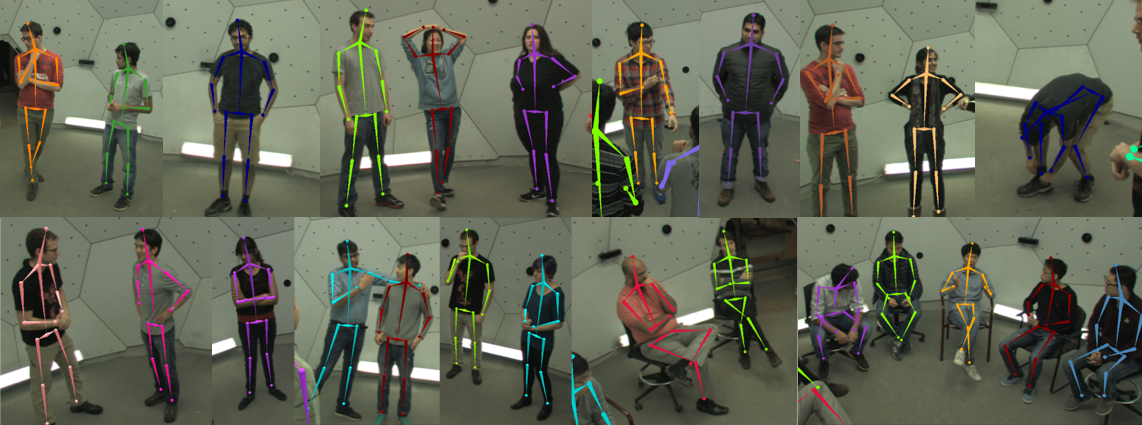
\includegraphics[width=\linewidth]{figures/iconicSocialPose}
	\caption{HD example views showing frequently occurring postures that carry rich social signals, with 3D body pose automatically annotated by our method.} 
	\label{fig:iconicPoses}
\end{figure}

\section{Method Overview and Notation}
Our algorithm is composed of two major stages. The first stage takes, as input, images from multiple views at a time instance (calibrated and synchronized), and produces 3D body skeletal proposals for multiple human subjects. The second stage further refines the output of the first stage by using a dense 3D patch trajectory stream~\cite{Joo2014}, and produces temporally stable 3D skeletons and an associated set of labeled 3D patch trajectories for each body part, describing subtle surface motions.

In the first stage, a 2D pose detector~\cite{Wei2016} is computed independently on all 480 VGA views at each time instant $t$, generating detection score maps for each body joint (see Fig.~\ref{fig:overview_mocap}b). The 2D score maps for each body joint~$j\in\{1,\cdots,J\}$ are combined into a 3D score map $H_j(\mathbf{Z})$ by projecting a grid of voxels $\mathbf{Z}\in \mathds{R}^3$ onto the 2D score maps and computing an average 3D score at each voxel (subsection~\ref{subsection:nodeProposals}).
%In the first stage, we consider a single time instant $t$ and drop the time variable for clarity. A 2D pose detector~\cite{Wei-2016} is computed on all 480 VGA images and generates detection score maps for each body joint (see Fig.~\ref{fig:overview}b). The 2D score maps for each body joint~$j$ are combined into a 3D score map $H_j(\mathbf{Z})$ by projecting a grid of voxels $\mathbf{Z}\in \mathds{R}^3$ onto the 2D score maps, computing an average 3D score (subsection~\ref{subsection:nodeProposals}).
%In the first stage, we will consider a single time instant $t$ and drop the time variable for clarity. To produce evidence of the location of different anatomical landmarks, our algorithm runs, on each of the 480 VGA views, a state-of-the-art 2D human pose detector~\cite{Wei-2016}. Each person detection comprises 15 anatomical landmarks or \emph{nodes} (3 for the head/torso and 12 for the limbs) and is associated with 2D heat maps~$h_{ij}^{c}(\mathbf{z})$ representing the detection score for node $j$ of the $i$-th person detection in camera $c$ at pixel ${\mathbf{z}}\in \mathds{R}^2$.  We combine all 2D heat maps for node $j$ into a 3D heat map $H_j(\mathbf{Z})$ by discretizing the volume into a grid of voxels $\mathbf{Z}\in \mathds{R}^3$, and projecting each voxel onto the 2D heat maps. The 3D score is the average over views $c$ of the maximum score across all detections~$i$.
%To produce evidence of the location of different anatomical landmarks, in the first stage, our algorithm runs a state-of-the-art 2D human pose detector~\cite{Wei-2016} on each of the up to 480 different viewpoints from the VGA cameras. The $i$-th 2D skeleton in a camera view $c$ at time $t$ is denoted by $s_{it}^c \in \mathds{R}^{30}$, and is composed of fifteen 2D anatomical landmarks or \emph{nodes} (3 for the head/torso and 12 for the limbs). Since the first stage of our method is performed at each time independently, we will consider a fixed time instant $t$, and drop the time variable for clarity. The $j$-th node of $s_{i}^c$ is denoted by $s_{i}^c(j) \in \mathds{R}^{2}$. The method of \cite{Wei-2016} also provides a heat map representing the per-pixel detection confidence for each node $s_{i}^c(j)$, which we denote as $h_{ij}^{c}(z)$, where ${z}\in \mathds{R}^2$ indexes 2D image space. We also save a merged version of 2D heatmap $h_j^{c}(z)$ for each joint $j$ at each view $c$ by taking the maximum over all person detections $i$ in $h_{ij}^{c}(z)$. The 2D score maps of node $j$ from all views are then combined into a 3D score map $H_j({Z})$, where ${Z}\in \mathds{R}^3$ indexes 3D space.\red{This seems incomplete. Reference details below?} 

Our approach then generates several levels of proposals, as shown in Figure~\ref{fig:overview}. A set of \textit{node proposals} $\mathbf{N}_j$ for each joint $j$ is generated by non-maxima suppression of the 3D score~map~$H_j(\mathbf{Z})$, where the $k$-th node proposal~$\mathbf{N}_j^k \in \mathds{R}^{3}$ is a putative 3D position of that anatomical landmark. Similarly, the set of \textit{part proposals} is denoted by $\mathbf{P}_{uv}$, where $u$ and $v$ are joints and $(u,v) \in \mathbf{B}$ is the set of body parts or {\em bones} composing a skeleton hierarchy.
%Because our skeleton is a tree structure and has fifteen nodes, $| \mathbf{B} | = 14$.
The $k$-th part proposal, $\mathbf{P}_{uv}^k= (\mathbf{N}_u^{k_u}, \mathbf{N}_v^{k_v}) \in \mathds{R}^6$, is a putative body part connecting two node proposals, $\mathbf{N}_u^{k_u}$ and $\mathbf{N}_v^{k_v}$, where the index $k$ enumerates all possible combinations of $k_u$ and $k_v$. As the output of the first stage, our algorithm produces \textit{skeletal proposals}; we refer to the $k$-th proposal as $\mathbf{S}^k = \{\mathbf{P}_{uv}^{k}\}_{uv \in \mathbf{B}}$. A skeletal proposal is generated by finding an optimal combination of part proposals using a dynamic programming method under the score function defined in subsection~\ref{subsection:dynamicProgamming}. Here, we abuse the notation to have $\mathbf{P}_{uv}^{k}$ refer to the optimally assigned part $u,v$ of skeleton $k$ (the superscript $k$ is understood to be the optimal mapping, from context). After reconstructing skeletal proposals at each time $t$ independently, we associate skeletons from the same identities across time and generate \textit{skeletal trajectory proposals} $\mathbf{\tilde{S}}^k(t) = \{\mathbf{\tilde{P}}^k_{uv}(t)\}_{uv \in \mathbf{B}}$, where $\mathbf{\tilde{P}}^k_{uv}(t)$ is a \textit{part trajectory proposal}, a moving part across time, with $k$ similarly overloaded to denote the optimal associations determined in each frame $t$.


%Our approach then generates several levels of proposals, as shown in Figure~\ref{fig:overview}. A set of \textit{node proposals} for landmark $j$ is denoted by $\mathbf{N}_j$, and is generated by non-maxima suppression of the score~map~$H_j(\mathbf{Z})$. The $k$-th node proposal~$\mathbf{N}_j(k) \in \mathds{R}^{3}$ is a putative 3D position of that anatomical landmark. Similarly, the set of \textit{part proposals} is denoted by $\mathbf{P}_{uv}$, where $(u,v) \in \mathbf{B}$ is the set of all parts composing a skeleton hierarchy. Since our skeleton is a tree structure and has fifteen nodes, $| \mathbf{B} | = 14$. The $k$-th part proposal, $\mathbf{P}_{uv}(k)= (\mathbf{N}_u(k_1), \mathbf{N}_v(k_2)) \in \mathds{R}^6$, is a body part connecting two node proposals, $\mathbf{N}_u(k_1)$ and $\mathbf{N}_v(k_2)$. As the output of the first stage, our algorithm produces \textit{skeletal proposals}; we refer to the $k$-th proposal as $\mathbf{S}(k) = \{\mathbf{P}_{uv}^k({k_{uv}})\}_{uv \in \mathbf{B}}$. A skeletal proposal is generated by finding the optimal combination of part proposals using a dynamic programming method under the score function defined in subsection~\ref{subsection:dynamicProgamming}. After reconstructing skeletal proposals $\mathbf{S}_t$ at each time $t$, we associate skeletons from the same identities across time and generate \textit{skeletal trajectory proposals} $\mathbf{\tilde{S}}(k) = \{\mathbf{\tilde{P}}^k_{uv}\}_{uv \in \mathbf{B}}$, where $\mathbf{\tilde{P}}^k_{uv}$ is a \textit{part trajectory proposal}, a moving part across time.


In the second stage, we refine the skeletal trajectory proposals generated in the first stage using dense 3D patch trajectories~\cite{Joo2014}. To produce evidence of the motion of different anatomical landmarks, we compute a set of dense 3D trajectories $\mathbf{F}=\{\mathbf{f}_i\}_{i=1}^{N_F}$, which we refer to as a \textit{3D patch trajectory stream}, by tracking each 3D patch independently. Each patch trajectory $f_i$ is initiated at an arbitrary time (every 20th frame in our results), and tracked for an arbitrary duration (30 frames backward-forward in our results) using the method of Joo et al. \cite{Joo2014}. Our method associates a part trajectory $\mathbf{\tilde{P}}^k_{uv}$ with a set of patch trajectories $\mathbf{F}_{uv}^k$ out of $\mathbf{F}$, and these trajectories determine rigid transformations, $T(t{+}1\,|\,t) \in SE(3) $, between any time $t$ to $t{+}1$ for this part. These labeled 3D trajectories associated to each part provide surface deformation cues and also play a role in refining the quality by reducing motion jitter, filling missing parts, and detecting erroneous parts.




\begin{figure}[t!]
	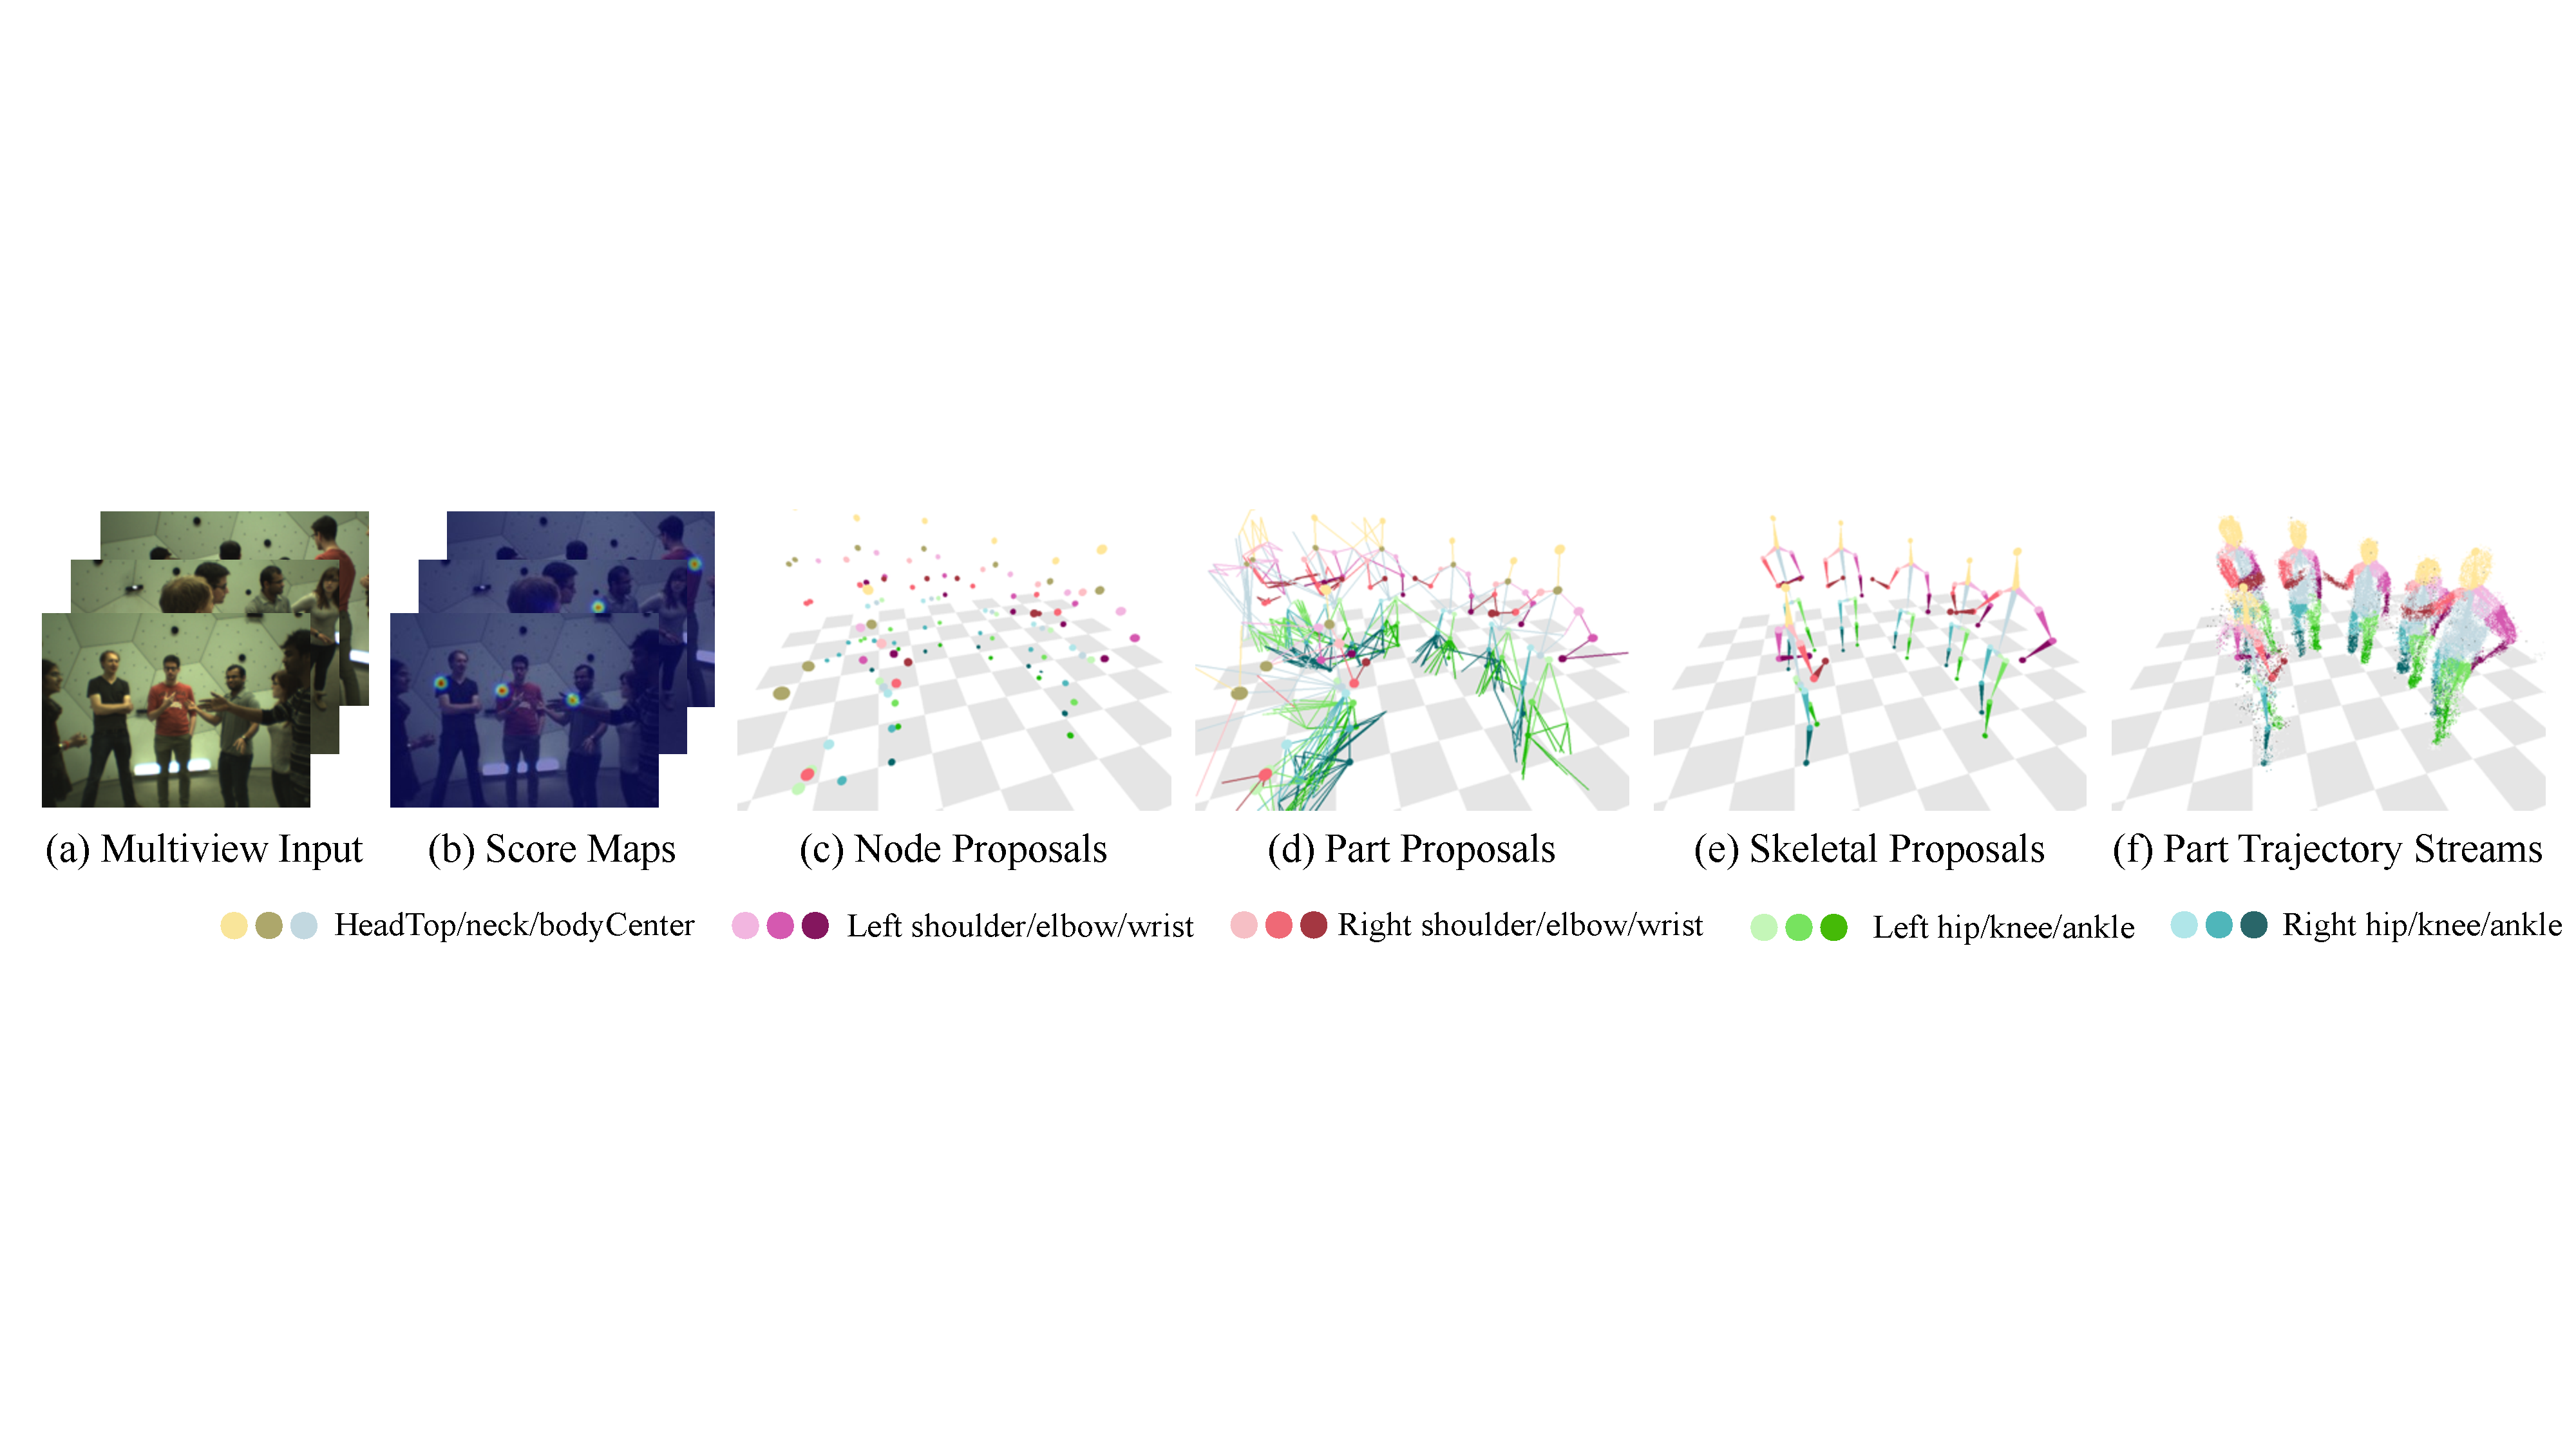
\includegraphics[width=\linewidth]{figures/overview2}
	%\includegraphics[width=\linewidth]{images/Design6.pdf}
	\caption{Several levels of proposals generated by our method. (a) Images from upto 480 views. (b)~Per-joint detection score maps. (c)~Node proposals generated after non-maxima suppression. (d)~Part proposals by connecting a pair of node proposals. (e)~Skeletal  proposals generated by piecing together part proposals. (f)~Labeled 3D patch trajectory stream showing associations with each part trajectory. In~(c-f), color means joint or part labels shown below the figure.} 
	\label{fig:overview_mocap}
\end{figure}

\begin{table}[t]	
	\renewcommand{\arraystretch}{1.3}
	\caption{Summary of Notation.}
	\label{Table:notations}
	\centering
	\begin{tabular}{l|l}
		\hline 
		Notation & Descriptions \tabularnewline
		\hline 	
		$s_{i}^c $ & $i$-th 2D skeleton detection in a camera view $c$ \tabularnewline		
		\hline 
		$s_{ij}^c $ & $j$-th joint of $i$-th 2D skeleton in a camera view $c$  \tabularnewline		
		\hline 
		$h_{ij}^{c}(\mathbf{z})$ & 2D score map of $j$-th joint of $i$th skeleton in view $c$  \tabularnewline		
		\hline 
		$h_{j}^{c}(\mathbf{z}) $ & Merged score map of $j$-th joint of all skeletons in view $c$  \tabularnewline		
		\hline 
		${H}_{j}(\mathbf{Z})$ & 3D score map for the $j$-th joint \tabularnewline		
		\hline 
		$\mathbf{N}_j$ & Node proposals for the $j$-th joint\tabularnewline		
		\hline 
		$\mathbf{P}_{uv}$ & Part proposals for the part connecting nodes $(u,v)$ \tabularnewline		
		\hline 
		$\mathbf{S}$ & Skeletal proposals connecting multiple part proposals \tabularnewline		
		\hline 
		$\mathbf{\tilde{S}}(t)$ & Skeletal trajectory proposals, associated through time  \tabularnewline		
		\hline   
		$\mathbf{\tilde{P}}_{uv}(t)$ & Part trajectory proposals for the connecting nodes $(u,v)$ \tabularnewline		
		\hline 
		$\mathbf{F}$	& 3D Patch Trajectory Stream, $\{\mathbf{f}_i\}_{i=1}^{N_F}$  \tabularnewline		
		\hline   
		$\mathbf{F}_{uv}$	& A subset of  $\mathbf{F}$ associated to $\mathbf{\tilde{P}}_{uv}$ \tabularnewline		
		\hline   
	\end{tabular} 
\end{table}




\begin{figure}[t]
	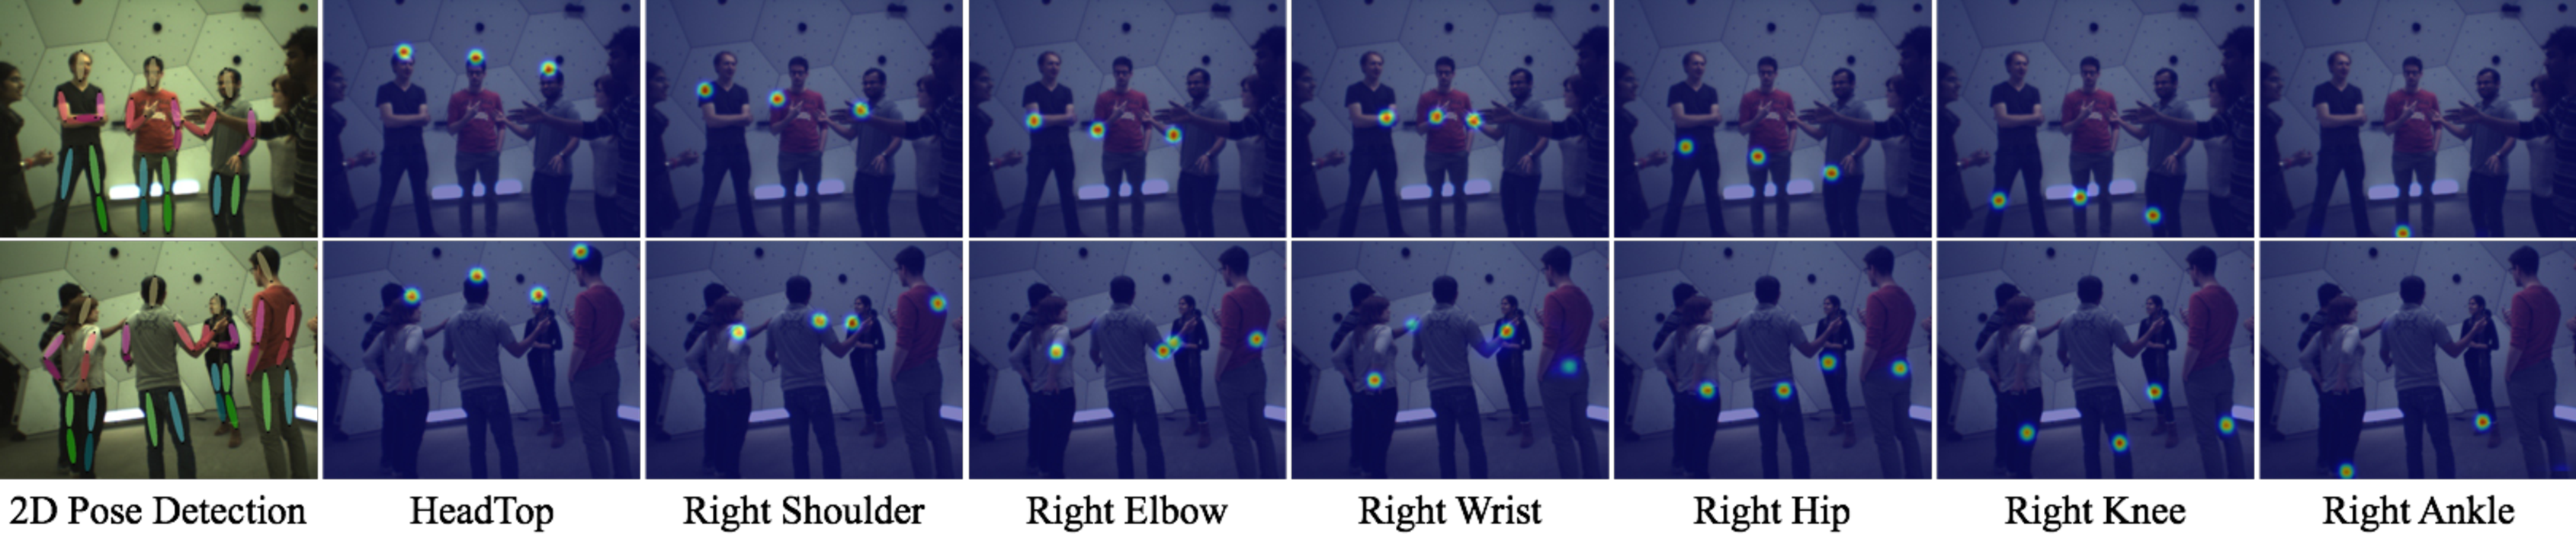
\includegraphics[width=\linewidth]{figures/HeatMaps3}
	%\includegraphics[width=\linewidth]{images/Design6.pdf}
	\caption{2D pose detections and score maps generated by the method of \cite{Wei2016}. (Column 1) Example views out of 480 views with proposals by the pose detector (Column 2-7) Heat maps for each node on each view. Note that the body pose detector distinguishes left-right limbs.}\label{fig:poseDetection}
\end{figure}
\section{The First Stage: Skeletal Proposals Generation}
%Our algorithm takes advantage of recent advances in 2D body pose detection by running a state-of-the-art detector in all the views of our massively multiview system and fusing the 2D cues in 3D space to estimate 3D skeletal poses at each time instance. 
Our algorithm integrates 2D pose detections across the many views of our massively multiview system, fusing simple 2D cues to estimate 3D skeletal poses at each time instance.
While detections in any single view may be incomplete or inaccurate---typically due to occlusions---we find that aggregating these cues across many views yields very stable results. Our method is simple, yet robust thanks to the large number of views. In contrast, prior marker-less motion capture methods are typically ``model-dependent'', requiring a 3D template model to constrain shape deformations, a motion model to constrain temporal deformations, and a relatively complex energy function minimization that trades off each of these priors~(e.g., \cite{Gall-09,Furukawa-2008, Elhayek-16}). Our method in this stage is essentially based on triangulating detections at a single time instance, and, thus, does not suffer from error accumulation or drift. It does not require a 3D template model, prior assumptions about the subject or the motion, or an initial alignment for tracking. In this section, we describe how the proposals are generated and built up from 2D cues.  
%Importantly, its simplicity makes it trivially parallelizable, allowing us to run it on long sequences with complex social interactions. 
%Our method is free from almost all prior knowledge about the scene and target subject (color, texture, height, shape, bone length, number of people, topology), and works generally well in variety of scenes by producing accurate skeletal proposals of multiple people for very long sequences. In this section, we describe how the skeletal proposals are built from 2D cues in multiple views. 

%We adopt an incremental approach to estimating skeletal motion, fusing appearance and motion cues across the set of views. In this section, we describe how the proposals are generated and built upon from these cues. 


\subsection{3D Node Score Map and Node Proposals}
\label{subsection:nodeProposals}
A single-view 2D pose detector is computed on all VGA views at each time instant, and is used to generate 2D pose detections and per-joint score maps in each image. Because the first stage of our method is performed at each time independently, we will consider a fixed time instant $t$, and drop the time variable for clarity. We use the detector of Wei et al.~\cite{Wei2016} without additional training. The method of \cite{Wei2016} requires bounding box proposals for each human body as initialization, thus, we first apply a person detector similar to R-CNN \cite{Girshick-14}, and run the pose detector on the detected person proposals represented as bounding boxes. Each 2D skeleton detection $i$ in a camera view $c$ is denoted by $\mathbf{s}_{i}^c \in \mathds{R}^{2\times 15}$, and is composed of 15 anatomical landmarks or \emph{nodes} (3 for the head/torso and 12 for the limbs), also referred to as joints\footnote{We modify the skeleton hierarchy of \cite{Wei2016} to have an explicit torso bone, by taking the center of the two hip nodes as a body center node.}. The position of the $j$-th node of the $i$-th person detection is denoted by $\mathbf{s}_{ij}^c \in \mathds{R}^{2}$. The method of \cite{Wei2016} also provides a score map representing the per-pixel detection confidence for each node $s_{ij}^c$, which we denote as $h_{ij}^{c}(\mathbf{z})\in[0,1]$, where $\mathbf{z}\in \mathds{R}^2$ indexes 2D image space. We also compute a merged score map by taking the maximum across all person detections at each pixel, $h_{j}^{c}(\mathbf{z})=\max_i h_{ij}^{c}(\mathbf{z})$. Merged score maps of example views are shown in Figure~\ref{fig:poseDetection}.

%The 2D score maps of node $j$ from all views are then combined into a 3D score map $H_j(\mathbf{Z})$, where $\mathbf{Z}\in \mathds{R}^3$ indexes 3D space.

%The output of the pose detector for each person proposal is a set of heat maps corresponding to each body node (14 joints in total) with peak locations of a single person. Since each image may have multiple people, we save heatmaps $h_{ij}^{c}(\mathbf{z})$ for each detected person $i$ with node $j$ in camera $c$. We also calculate a merged heatmap by taking the maximum across all detections at each pixel, $h_{j}^{c}(\mathbf{z})=\operatorname{max}_i h_{ij}^{c}(\mathbf{z})$. Each 2D skeleton $s_{i}^c $ in a view $c$ contains a tree-like skeletal hierarchy composed of 15 nodes. Note that we have a 2d score heatmap $h^{c}_j$ for each node and for each view. Since the method of \cite{Wei-2016} shows excellent performance in distinguishing person-centric left/right limbs, we also distinguish them, keeping the score maps of left/right limbs separately, which ends up with 15 score heatmaps (3 for head/torso nodes, and 12 for limbs) in each view. Score maps of example views are shown in Figure~\ref{fig:poseDetection}.

%Since our method in this stage work on a single each time independently, we will consider a fixed time $t$ in this section. 

%The score map of a node $j$ in a view $c$ is defined as 
%\begin{equation}
%\mathbf{\phi}_j^c(z)=\max_i \alpha^c_i \mathcal{G}(z~|~s_{ij}^c,\sigma^c_i),
%\end{equation}
%where $z \in \mathds{R}^2$ is a 2D location, and $\mathcal{G}$ is a Gaussian kernel centered on $s_{ij}^c$ with covariance $\sigma^c_i$, and scaled by the detection score $\alpha^c_i$.

 %Although the pose detection results are highly reliable, there exists cases where it failed due to the occlusions among people or self-occlusions. These failures can be robustly handled once we fuse the 2d cues multiple views in 3D. 

To combine 2D node score maps from multiple views into 3D, we generate a 3D score map for each node using a spatial voting method. We first index the 3D working space into a voxel grid (4cm in our implementation), and compute the \textit{node-likelihood} score of each voxel by projecting the center of the voxel to all views and taking the average of the 2D scores at the projected locations. The 3D score map $H_j(\mathbf{Z})$ for a node $j$ at the 3D position $\mathbf{Z}\in\mathds{R}^3$ is defined as 
\begin{equation}
{H}_j(\mathbf{Z}) = \frac{1}{ | V(\mathbf{Z}) | } \sum_{c \in V(\mathbf{Z})} {h^c_j \left(\mathcal{P}_c({\mathbf{Z}}) \right) }  ,
\end{equation}
where $\mathcal{P}_c(\cdot)\in\mathds{R}^2$ denotes projection into camera~$c$, $V(\mathbf{Z})$ is the set of cameras where the 3D location $\mathbf{Z}$ is visible, and $| V(\mathbf{Z}) |$ is the cardinality of the set. Note that the 3D score map for each node is computed separately, producing fifteen 3D score maps at each time instant. 
%We perform this process at every frame independently. %When the pose detector is unreliable, we found that taking summation is better than average, but in our case with the state-of-art detector, we find that summation and average have similar performance, but we chose the average score since it is better in selecting thresholds. 

From the 3D score map for each node at each time instance, we perform Non-Maxima Suppression (NMS), and keep all the candidates above a fixed threshold $\tau$ (we use $\tau{=}0.05$). The results are shown in the Figure~\ref{fig:overview}c, and the same results color-coded by the node scores are shown in Figure~\ref{fig:proposalScores}. Each node proposal, denoted as $\mathbf{N}_j^k$ for the $k$-th proposal for node $j$, is a putative candidate for the $j$-th anatomical landmark of a participant.

%The generated 3D node score maps and node proposals play two meaningful roles: (1) Initial node locations by which we can perform dynamic programming to construct skeletons; (2) It provides association among 2D peak locations across views which allows us to perform further optimization to minimize reprojection error. This is described in subsection XX. %Since we can perform the additional optimization to refine the 3D location of each joint, we can use coarse voxel grid, and we use 4cm voxel here. 

\subsection{Part Proposals}
\label{subsection:partProposals}

Given the generated node proposals, we infer part proposals by estimating connectivity between each pair of nodes that make up a possible body part. The 2D detector \cite{Wei2016} uses appearance information during the inference, and, thus, the result tends to preserve connectivity information (e.g., left knee is connected to the left foot of the same person). Our approach fuses them by voting 2D connectivity into 3D. More specifically, we define a connectivity score between a pair of node proposals by projecting them onto all views, and checking in how many views they are actually connected, i.e., both nodes belong to the same person detection. Formally, the connectivity score of a part $\mathbf{P}_{uv}^k$ between two node proposals $( \mathbf{N}_{u}^{k_u}, \mathbf{N}_{v}^{k_v})$, where $(u,v) \in \mathbf{B}$, is defined as
\begin{gather}
%\mathbf{L}( \mathbf{P}_{uv} )=  \sum_{c} \delta^c_{uv} \left( \frac{\mathbf{M}^c \mathbf{\hat{N}}^{k_1}_{u}}{(\mathbf{M}^c \mathbf{\hat{N}}^{k_1}_{u} )_3}, \frac{\mathbf{M}^c \mathbf{\hat{N}}^{k_2}_{v}}{(\mathbf{M}^c \mathbf{\hat{N}}^{k_2}_{v})_3}\right), \nonumber 
{\Phi}( \mathbf{P}_{uv}^k )=  \frac{1}{ | V( \mathbf{P}_{uv}^k ) | } \sum_{c \in V(\mathbf{P}_{uv}^k)}   \max_{i} \phi_{iuv}^c \left( \mathcal{P}_c(\mathbf{N}^{k_u}_{u}),\mathcal{P}_c(\mathbf{N}^{k_v}_{v}) \right), \nonumber \\
\phi_{iuv}^c(\mathbf{z}_u,\mathbf{z}_v) = w_{iuv}^c(\mathbf{z}_u,\mathbf{z}_v)\delta^c_{iuv} \left(\mathbf{z}_u,\mathbf{z}_v \right) \nonumber
%w_{uv}^c(z_u^{k_1}, z_v^{k_2})\delta^c_{uv} \left( i, z_u^{k_1}, z_v^{k_2} \right)
% 
% \mathbf{M}^c(\mathbf{N}^{k_1}_{u}), \mathbf{M}^c(\mathbf{N}^{k_2}_{v}) 
%  
%h_{iu}^c(\mathbf{M}^c(\mathbf{N}^{k_1}_{u})) + h_{iv}^c(\mathbf{M}^c(\mathbf{N}^{k_1}_{u})) 
%}{(\mathbf{M}^c \mathbf{\hat{N}}^{k_1}_{u} )_3}, \frac{\mathbf{M}^c \mathbf{\hat{N}}^{k_2}_{v}}{(\mathbf{M}^c \mathbf{\hat{N}}^{k_2}_{v})_3}\right), \nonumber 
\end{gather}
where
\begin{align}
w_{iuv}^c(\mathbf{z}_u,\mathbf{z}_v) &= \frac{1}{2}\left(h_{iu}^c(\mathbf{z}_u) + h_{iv}^c(\mathbf{z}_v) \right), \text{and} \nonumber\\
\delta^c_{iuv}( \mathbf{z}_u ,\mathbf{z}_v) &=  \begin{cases}
1 & \mathrm{if}\,\, h_{iu}^c( \mathbf{z}_u ) > \tau ~\mathrm{and}~h_{iv}^c( \mathbf{z}_v ) > \tau\\
0 & {\mathrm otherwise}.
\end{cases} \nonumber
\end{align}
Here, $\mathcal{P}_c(\mathbf{N}^{k_u}_{u})$ and $\mathcal{P}_c(\mathbf{N}^{k_v}_{v})$ are the projections of the two nodes of $\mathbf{P}_{uv}^k$ in view $c$, and $ V( \mathbf{P}_{uv}^k )$ is the set of cameras where the 3D part is visible. Intuitively, the part score ${\Phi}$ represents the average connectivity score across all views from all potentially corresponding 2D person detections. Because we do not know the correspondence from 3D parts to 2D person detections, we take the maximum score across all possible detections $i$ in each view. Assuming that the projected part corresponds to the $i$-th person detection in camera $c$, the part connectivity score %The function $\phi_{iuv}^c$ defines the connectivity score for the part proposal when projected on camera $c$, and $i$ iterates over all skeleton detections in that view.
$\phi_{iuv}^c$ is defined as the average score of the projected nodes, denoted by $w_{iuv}^c(\mathbf{z}_u,\mathbf{z}_v)$. The delta function $\delta^c_{iuv}$ additionally ensures that $\phi_{iuv}^c$ is nonzero only if both projected node locations have a sufficiently high score for the same detection $i$ (i.e., both nodes are detected as part of a single person). An example of computed part scores is shown in Figure~\ref{fig:proposalScores}.
%If the part proposal is actual an body part, there are many detections supporting the connectivity with high heat map score value. In contrast, if a pair of node is not a valid body part, the score becomes low although each node score has high score values because not many 2D skeletons support connection for the part. In this case, for example, the average of heat map score $w_{iuv}$ may have large value, but the delta function should be off. 
%$\phi_{iuv}^c$ is defined by the multiplication of an averaged 2D heat map score $w_{iuv}^c(z_u,z_v)$ and a delta function $\delta^c_{iuv}$. The $w_{iuv}^c(z_u,z_v)$ is the average of heat map scores of corresponding nodes, $u$ and $v$ here, of the $i$-th skeleton. The delta function $\delta^c_{iuv}$ is on only if both projected location has sufficiently high score in the heat map, meaning that the connectivity of the projected 2D part is supported by the detected $i$-th skeleton. Note that 2D heat maps, $h_{iu}^c$ and $h_{iv}^c$, correspond to the same $i$-th detection. Intuitively, the 3D part score $\mathbf{\Phi}$ represents the average of 2d connectivity score from all potentially corresponding 2D skeletons. If the part proposal is actual body part, there are many corresponding 2D skeletons supporting the connectivity with high heat map score value. In contrast, if a pair of node is not a valid body part, the score becomes low although each node score has high score values because not many 2D skeletons support connection for the part. In this case, for example, the average of heat map score $w_{iuv}$ may have large value, but the delta function should be off. An example of computed part score is shown in Figure~\ref{fig:proposalScores}.


\subsection{Generating Skeletal Proposals by Dynamic Programming}
\label{subsection:dynamicProgamming}


\begin{figure}
	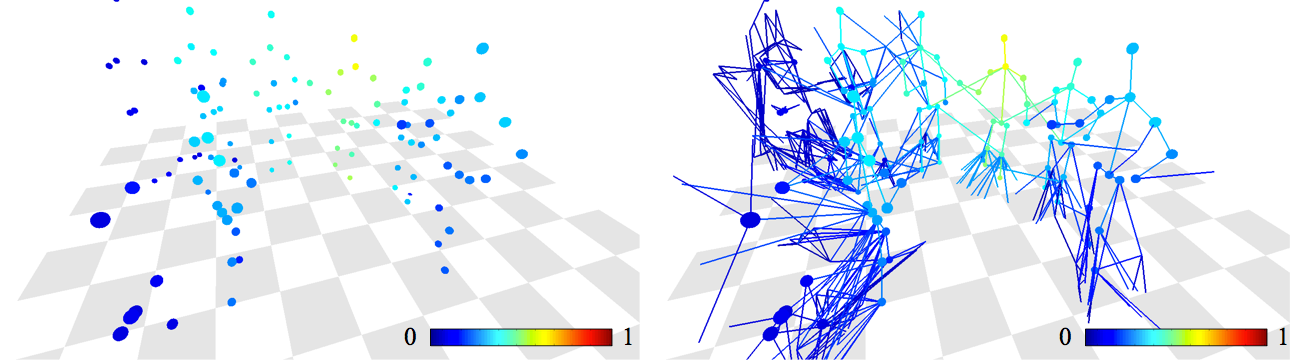
\includegraphics[width=\linewidth]{figures/ProposalScores}
	%\includegraphics[width=\linewidth]{images/Design6.pdf}
	\caption{Computed scores for node proposals and part proposals. The color encodes scores.} 
	\label{fig:proposalScores}
\end{figure}

Our method generates skeleton proposals by piecing together the part proposals. Since each skeleton is a tree structure, this can be computed efficiently using Dynamic Programming (DP)---but only for a single person. Therefore, we use DP to greedily find 3D skeletons $\mathbf{S}^k$ which maximize the sum of part scores,
\begin{gather}
%\Theta_{\mathbf{S}} (\mathbf{S}^k)= \sum_{u \in \mathbf{Skel}} \Phi_{u}(\mathbf{Z}_u) +  \lambda \sum_{(u,v) \in \mathbf{B}} \mathbf{L} \left( \mathbf{P}_{uv} \right), \nonumber
\Theta (\mathbf{S}^k)= \max_{(k_{1},\cdots,k_J)}\sum_{(u,v) \in \mathbf{B}} {\Phi} \left( \mathbf{P}_{uv}^{k} \right). \nonumber
\end{gather}
A skeleton $\mathbf{S}^k$ is given by the mapping $k\mapsto(k_1,\cdots,k_J)$, where the J-tuple $(k_1,\cdots,k_J)$ determines the assignment of node proposals $\mathbf{N}_j^{k_j}$ for each joint $j$ in the body. After picking the highest scoring skeleton $\Theta(\mathbf{S}^k)$, the assigned nodes $(k_1,\cdots,k_J)$ are removed from the pool of available node proposals and we run DP again to find the next highest scoring skeleton, and so on until all possible skeletons are found.

One option here would be to threshold the skeleton scores $\Theta(\mathbf{S}^k)$ at some minimum value to determine valid detections. However, we can do better: each 3D skeleton  should be supported by 2D detections, and each 2D detection can correspond to only a single 3D skeleton. This observation is important because the voting used to generate 3D node proposals assigns equal score to {\em all} voxels along the line of sight of each 2D detection (Sect.~\ref{subsection:nodeProposals}), and, similarly, the $\max$ over detections in the part score $\Phi(\cdot)$ makes  $\Theta(\mathbf{S}^k)$ an overestimate. 
%Note that the score function only has unary terms for each part and lacks pairwise terms, distinguishing it from other 3D Pictorial Structure (3DPS) methods. Our method does not use any bone length priors, and, thus, it does not use a pairwise spring model. This shows a big advantage in applying the method to subjects of arbitrary height---we demonstrate results ranging from toddlers to tall adults.
%Although we have scores associated with each node, our formulation does not explicitly use a node score because the part score already captures this value (it is the average node score of the end points). After generating all possible skeletal proposals, we perform NMS and retain the best local skeletons. 

To avoid this form of double counting, our method places each 3D node $\mathbf{N}^{k}_{j}$ in skeleton $\mathbf{S}^k$ in correspondence with the closest 2D joint detection in each view. For each 3D node $\mathbf{N}^{k}_{j}$, we create a set of correspondences $\mathcal{C}_j^k$ with elements $(c,i)$ such that the distance $\| \mathcal{P}_c(\mathbf{N}_j^k) - \mathbf{s}_{ij}^c \|_2$ is the minimum across all detections $i$ in view $c$ and smaller than $\delta{=}10$px. 
Once a 2D correspondence is established, we remove it from the set of available 2D detections, and, as above, this is performed greedily in order of decreasing skeleton score $\Theta(\mathbf{S}^k)$. Skeletons where the head node has fewer than two correspondences are discarded, i.e., if $|\mathcal{C}_{j}^k|<2$ for $j$ the head.

We additionally use the set of correspondences $\mathcal{C}_j^k$ to refine the 3D node locations by minimizing reprojection error. This overcomes the discretization error introduced by the voxel grid resolution. The final 3D node location $\hat{\mathbf{N}}^{k}_{j}$ is then
\begin{gather}
\hat{\mathbf{N}}^k_j = \arg\min_\mathbf{Z} \sum_{(c,i) \in \mathcal{C}_j^k} \left\|\mathcal{P}_c(\mathbf{Z}) - \mathbf{s}_{ij}^c \right\|_2. \nonumber
\end{gather}
The output of the algorithm described in this section is 3D skeletal proposals reconstructed independently at each time instance. After performing this process on all frames, our method associates skeletons from the same identity across time by simply considering spatial distance of the head node. That is, for a $\mathbf{S}_t^{k_1}$ reconstructed at time $t$, we find a corresponding skeleton at $\mathbf{S}_{t+1}^{k_1}$ with the closest head node location from $\mathbf{S}_t^{k_1}$ within a threshold. 
%We find this simple association works well in practice, since head parts are reconstructed reliably and false positive skeleton detections that are near true detections are filtered out by NMS. 
To be somewhat robust to missing skeleton detections, our method associates across a window of time. If there is no corresponding skeleton at time $t+1$, we also consider the next time $t+2$ and find a corresponding skeleton.
% to missing detections. 
%This missing holes can be filled using the method described in the next section using temporal cues from 3D patch trajectory streams. 

%It should be noted that our method is highly general without using prior assumptions such color, texture, height, shape, bone length, and number of people in the scene, which is suitable for social study where diverse subjects can be participated. 
This first stage of our method is performed without considering any temporal cues. The advantages of this are that the method can easily handle a varying number of people, there is no need to impose priors on the motion or skeletons, and the bulk of the computation is easily parallelized across frames. In many cases, we find that the results from the first stage are already sufficient for many applications. However, the results exhibit some jitter---especially for complex scenes with limited views per person---and missed or noisy detections do not benefit from evidence found in adjacent frames. We address these issues in the second stage of our method.

\section{The Second Stage: Temporal Refinement and Trajectory Stream Labeling}
The per-frame skeletal proposals from the first stage can be improved by using temporal coherence. We use motion cues from a {\em 3D patch trajectory stream}: dense 3D point tracks computed by the method of Joo et al.~\cite{Joo2014}. We find an association between each part trajectory proposal and a subset of the patches in the trajectory stream, and use it to reduce motion jitter, remove false detections, and fill in missing detections. The resulting labeled patch trajectories also capture rich motion information representing the subtle deformations of the surface for each body part (see Fig.~\ref{fig:overview}f).

%\begin{figure}[t]
%	\centering       
%	\subfigure[Patch cloud]{\label{fig:patchCloud}\includegraphics[width=0.8\columnwidth]{imgs/patchTraj/patchCloud_normal}} 
%	\subfigure[A magnified view]{\label{fig:patch_magnifiedView}\includegraphics[width=0.8\columnwidth]{imgs/patchTraj/patchCloud_mag}} 
%	%	\subfigure[A selected part proposal]{\label{fig:partTrajectoryProposals2}\includegraphics[trim=70 0 70 0,clip,height=0.14\textwidth]{img/Proposals/partTrajectoryProposals3}}
%	\caption{2D body pose detection result on an example view.} 
%	
%	\label{fig:patchCloud}
%\end{figure}
%
%
%
%\begin{figure}[t]
%	\centering
%	\begin{subfigure}{\linewidth}
%	\includegraphics[width=0.8\columnwidth]{imgs/patchTraj/patchCloud_normal} 
%	\caption{Patch cloud}
%	\label{fig:patchCloud}
%	\end{subfigure}
%%	\subfigure[A magnified view]{\label{fig:patch_magnifiedView}\includegraphics[width=0.8\columnwidth]{imgs/patchTraj/patchCloud_mag}} 
%	%	\subfigure[A selected part proposal]{\label{fig:partTrajectoryProposals2}\includegraphics[trim=70 0 70 0,clip,height=0.14\textwidth]{img/Proposals/partTrajectoryProposals3}}
%	\caption{2D body pose detection result on an example view.} 
%	
%	\label{fig:patchCloud}
%\end{figure}

\subsection{Patch Trajectory Stream Reconstruction}
\label{subsection:patchTrajectoryRecon}
We can only observe surface motions, not the true motion of the underlying skeleton, so it is not immediately apparent how best to enforce temporal consistency in the motion of body parts. Clothing in particular makes the relationship between surface motion and body parts difficult to model. To keep the use of priors and models to a minimum, we therefore choose to measure surface motion independently from the underlying skeletal motion and postpone all decisions about part-to-surface associations.

To represent surface motion, we use the method of \cite{Joo2014} to track a dense 3D patch cloud---a set of points with corresponding surface normal and a small spatial extent, representing the surface locally---and estimate the motion of each of these patches. Instead of generating the initial patches to track using SIFT matching and triangulation (as in \cite{Joo2014}), we use the depth maps from our 10 RGB+D sensors to generate an initial set of 3D patches. For a single frame, a dense 3D point cloud is first generated from the depth maps, and planar local patches centered on each point are initialized. The size of patches is manually determined by considering image resolution and fixed for entire processes at {6cm$\times$6cm}. To find the normal of each patch, we apply Singular Value Decomposition (SVD) to the coordinates of points within a neighborhood (determined by Euclidean distance from the center point with the patch size as a threshold), and the least principal axis is selected as the normal direction. The sign of the normal is disambiguated by considering camera visibility. 

The remainder of the algorithm (3D patch tracking) is as described in~\cite{Joo2014}. As a brief overview, a patch is represented by a triplet points (the center point, and two orthogonal points on the patch plane), and it is tracked by projecting the triplet points on all views where the target patch is visible. Optical flow tracking is performed in 2D on each point, and the tracked 2D flows are triangulated into 3D. The core idea to fully leverage a large number of views is to reason about the time-varying camera visibility of each patch. The visibility is optimally estimated in a MAP framework that combines photometric consistency, motion consistency, and visibility priors, see \cite{Joo2014} for more details. For our results, we initialize a 3D patch cloud every 20th frame, and track them backward and forward for 30 frames in each direction. As output, we obtain a dense 3D patch trajectory stream, $\mathbf{F}=\{\mathbf{f}_i\}_{i=1}^{N_F}$, where each $\mathbf{f}_i(t)\in\mathds{R}^3$ is the time-varying position of a tracked patch.

\subsection{Associating Part Trajectory Proposals and Trajectory Stream}
\label{subsection:trajectoryAssociation}
Part trajectory proposals $\mathbf{\tilde{P}}_{uv}$ represent the moving body parts of a single person, and are given by the optimal assignment used to generate skeletal trajectory proposals. These part trajectories lack temporal coherence because they are reconstructed independently in each frame. However, the trajectory streams provide evidence of the motion of each limb, and can be used to refine the motion of each body part. We therefore find an association between each part trajectory proposal and a subset of patch trajectories. This can be seen as a semantic labeling of the patch trajectory stream with the corresponding body parts (see Fig.\ref{fig:overview}f). 

Before performing this association, we first remove erroneous part detections which can readily be identified as outliers. 
%These outliers are typically false positives and happen when the 2D detections are consistently wrong across multiple views (e.g., from unusual poses), or due to a lack of visibility (e.g., people standing near the edges of the capture space). 
We find that a simple yet robust method is to use the depth maps from the multiple RGB+D sensors. At any time instant, a part can be considered as an outlier if it is {\em outside} of every surface in the dense point cloud. We simply test this by checking whether a part proposal is in front of the measured depth in any view, and mark it as erroneous if it is. 
This is a necessary but not sufficient condition because we test this from only the 10 available depth map views.
%, although a part passes the test, it might still be an outlier. 
However, we find that this method works well in practice and is efficient to implement. After identifying these outliers, we remove and treat them as missing data. Then, we can assume that this filtered part trajectory only suffers from relatively small jitter and occasionally missing data. 

We associate a set of patch trajectories with a filtered part trajectory proposal if they move rigidly and the patch normal is a match. Intuitively, the part should be located inside the body surface, and, thus, a vector from the closest point on the part to the patch center should have a similar direction as the patch normal---their inner product should be positive. For a part trajectory proposal, we only consider patches for which the normal satisfies this criterion for the entire duration of the patch trajectory. As additional criteria, we compute a measure of rigidity between a patch trajectory and a part trajectory proposal. We define this as the difference between the minimum and maximum distance between them across all frames $t$ in which they overlap:
\begin{gather}
d(\mathbf{f}_i,\mathbf{\tilde P}_{uv}^k) = \max_t \, l\!\left(\mathbf{f}_i(t),\mathbf{\tilde P}_{uv}^k(t)\right)  - \min_t \, l\!\left(\mathbf{f}_i(t), \mathbf{\tilde P}_{uv}^k(t)\right),   \nonumber
\end{gather}
where $l( \cdot, \cdot )$ is the orthogonal distance between the patch center and the line segment of the body part, i.e.,
\begin{gather}
l\!\left(\mathbf{f}_i(t),\mathbf{\tilde P}_{uv}^k(t)\right) = \min_\alpha \| \alpha \mathbf{N}_{u}^{k_u}(t) {+}(1{-}\alpha)\mathbf{N}_{v}^{k_v}(t)  - \mathbf{f}_i(t)\|_2. \nonumber
\label{eq:segment_distance}
\end{gather}
Here, the set of time instants $t$ satisfies that both the patch trajectory and part trajectory streams are valid, and only patch trajectories $i$ for which $0{\leq}\alpha{\leq}1$ at some time $t$ are considered. Intuitively, this cost approximates how rigidly they move together over time, going to zero for completely rigid motion. Each part trajectory $\mathbf{\tilde{P}}^k_{uv}$ is then associated with a set of patch trajectories $\mathbf{F}^k_{uv}$, for which the rigidity cost is less than a threshold, i.e., $\mathbf{F}^k_{uv} = \{ \mathbf{f}_i : d(\mathbf{f}_i,\mathbf{\tilde P}_{uv}^k){\leq}10\textrm{cm}\}$. If a patch trajectory is selected by multiple body parts (e.g., a static scene as an extreme case), the trajectory is associated with the body part with minimum $\max_t \, l (\mathbf{f}_i(t),\mathbf{\tilde P}_{uv}^k(t) )$ distance. An example of this labeling is shown in Figure~\ref{fig:overview}f.

\subsection{Motion Refinement by Associated Patch Trajectories}
From the set of patch trajectories $\mathbf{F}_{uv}^k$ associated to the part trajectory proposal $\mathbf{\tilde{P}}_{uv}^k$, we can compute the rigid transform between subsequent time instances from $t$ to $t{+}1$, $T(t{+}1\left|\right.t) $, and, progressively, to any frame $t'$ by concatenating transformations between subsequent frames, so that $T(t'\left|\right.t)\mathbf{\tilde{P}}_{uv}^k(t)$ represents the propagated part from time $t$ to $t'$. Using the transformation it is possible to propagate a body part's position to other time instants. Our method uses the propagated parts to reduce jitter and fill in missing holes by averaging multiple part locations propagated from different time instances. For a target time $t$, we can produce multiple proposals for the same part, including the proposal from the first stage of our method and propagated parts using the estimated transformations, creating a set 
\begin{gather}
\{ T(t\left|\right.t{-}n) \mathbf{\tilde{P}}_{uv}^k(t{-}n),\cdots\!,\mathbf{\tilde{P}}_{uv}^k(t),\cdots\!,T(t\left|\right.t{+}n) \mathbf{\tilde{P}}_{uv}^k(t{+}n) \}.		\nonumber
\end{gather}
If there are elements in this set, we take the average. If the set is empty due to consistently severe occlusions, we determine that the part at time $t$ is still missing. In practice, we use $n{=}$1. This procedure can also be iterated multiple times (including patch trajectory re-association) to fill in missing parts that are further than $n$ frames from any part proposal. We iterate this refinement until no more missing parts can be filled. After refinement, a node connected to multiple body parts can have different locations corresponding to each of the averaged parts, and we simply take the average to determine the final node locations. It should be noted that our method is different from temporal smoothing (e.g., ~\cite{Elhayek-16}). Instead, we use an actual measurement of 3D motion rather than impose a motion prior, which prevents over-smoothing even after several iterations. 


\section{Face and Hand Captures}
In this section, we briefly describe the method to capture 3d motion of faces and hands given reconstructed body landmarks. By projecting 3D landmark locations of head and wrists on each view, approximate regions of hands and face are obtained. We then apply 2d face pose detector and 2D hand detector on each region to find 2D landmark locations. Correspondences of landmarks across views are already given by construction, and final 3D face and hand are reconstructed by triangulation with RANSAC. 

We use the hand detector we present in~\cite{simon2017hand}. The hand detector is based on the same Convolutional Neural Network architecture of ~\cite{Wei2016} which we used for 2D body pose detection, but trained on a hand keypoint dataset generated by Multiview Bootstrapping method proposed in \cite{simon2017hand}. Similarly, we also produce a 2D face detector using the same CNN architecture and a face dataset by Multiview Bootstrapping in the Panoptic Studio. We found that this method shows a comparable performance to the state-of-the-art methods and outperforms them in profile views.  Before applying detectors, occluded views are excluded by considering the orthogonal distance from camera rays and body skeletons, where thresholds is used to determine occlusion (15~cm for the metacarpals, 9~cm for the proximal phalanges, and 5~cm for the remaining bones). 


For a landmark location, we robustly triangulate it into a 3D location. We use RANSAC~\cite{Fischler-81} on points with confidence above a detection threshold $\lambda$. Additionally, we use a 4 pixel reprojection error to accept RANSAC inliers. With this set of inlier views for point, we minimize~\cite{ceres-solver} the reprojection error to obtain the final triangulated position. 

To improve robustness specifically for hands, we reconstruct entire fingers simultaneously. We triangulate all landmarks of each finger (4 points) at a time, and use the average reprojection error of all 4 points to determine RANSAC inliers. This procedure is more robust because errors in finger detections are correlated: e.g.,~if the knuckle is incorrectly localized, then dependent joints in the kinematic chain---the inter-phalangeal joints and finger tip---are unlikely to be correct. This reduces the number of triangulated keypoints (because the entire finger needs to be correct in the same view) but it further reduces the number of false positives, which is more important so that we do not train with incorrect labels. A similar approach is applied for face by grouping each eye, nose, and lip, and apply RANSAC respectively. 

\section{Results}

We quantitatively and qualitatively evaluate our method on various sequences captured in the Panoptic Studio. In the quantitative evaluation, we empirically show how the large number of views solves the challenging interaction capture problem; we compare performance using varying number of cameras on the scenes with different number of people. In the qualitative evaluation, we demonstrate the ``model-free" advantage of our method by showing compelling motion reconstruction results on subjects of diverse appearance, body shapes, and body sizes.

In this result section, we mainly focus on the performance of body motion capture, yet qualitative results of 3D face and hand captures are shown. 

%\subsection{Calibration/Sync Quality???} 
%\begin{itemize}
%	\item Checker board sequence
%	\item Leave-one-out test (1 pixel at most)
%\end{itemize}

% 	\begin{table} [t]	
% 		\centering
% 		\caption{Summary of Panoptic studio dataset. The second columns shows the number of subjects per scene with total number of subjects in the entire sequence (shown in the parenthesis). The fourth columns represent the number of reconstructed 3D skeletons. }\label{Table:socialDataset}

% 		\begin{tabular}{c|c|c|c}
% 			\hline 
% 			{Sequence Name} & {  \centering Subject \# } & { \centering  Duration } &Skeleton \#\tabularnewline
% 			\hline 
% 			\hline 	
% 			160422 mafia1 & 4-8  & 15 min   & 114K \tabularnewline		%150129_Ultimatum7
% 			\hline 
% 			160422 mafia2 & 7-8  & 15 min    & 135K \tabularnewline %134,625 		%150129_Ultimatum7
% 			\hline 
% 			160226 mafia1 & 7-8  & 10 min   & 92K \tabularnewline		%150129_Ultimatum7
% 			\hline 
% 			160226 mafia2 & 5-8 & 10 min  &  88K \tabularnewline	%87,882 	%150129_Ultimatum7
% 			\hline 
% 			160224 mafia1 & 4-7  & 8 min  & -\tabularnewline		%150129_Ultimatum7
% 			\hline 
% 			160224 mafia2 & 4-7  & 10 min  & 60K \tabularnewline		%150129_Ultimatum7
% 			\hline 
% 			151125 mafia1 & 4-8  & 10 min  & -\tabularnewline		%150129_Ultimatum7
% 			\hline 	
% 			160422 ultimatum1 & 2-8 & 15 min & 82K \tabularnewline %81,829		%150129_Ultimatum7 (11)
% 			\hline 
% 			160226 ultimatum1 & 2-8 & 14 min  & 68K \tabularnewline %67,725		%150129_Ultimatum7 (12)
% 			\hline 
% 			160224 ultimatum1 & 2-7  & 9 min & 44K \tabularnewline		%150129_Ultimatum7  (7)
% 			\hline 
% 			160224 ultimatum2 & 4-7 & 9 min& 46K \tabularnewline	%45,989	%150129_Ultimatum7 (7)
% 			\hline 
% 			160422 haggling1 & 3 & 8 min&  23K \tabularnewline %23,738		%150129_Ultimatum7
% 			\hline 
% 			160226 haggling1 & 3 & 8 min&  22K \tabularnewline	%22,060	%150129_Ultimatum7 (6) 
% 			\hline 		
% 			160224 haggling1 & 3  & 5 min &  15K \tabularnewline		%150129_Ultimatum7
% 			\hline 
% 			151125 007Bang &  6-7  &  5 min&  40K \tabularnewline	%40,235 	%150129_Ultimatum7
% 			\hline 	
% 			150129 007Bang  & 5 &  7  min&  26K  \tabularnewline	%25,891	%150129_Ultimatum7
% 			\hline 	
% 			160317 meeting1 & 6-8 & 10 min & 99K \tabularnewline		%150129_Ultimatum7
% 			\hline 				
% 			160401 ian3 &  2 & 5 min  & 10K \tabularnewline		%150129_Ultimatum7
% 			\hline 
% 			\hline 
% 			150821 dance1 & 1  &  3 min & 4K  \tabularnewline		%150129_Ultimatum7
% 			\hline 
% 			150821 dance3 & 1 &  5 min & 7K \tabularnewline		%150129_Ultimatum7
% 			\hline 	
% 			150303 cello4  & 1 &  5 min & 4K \tabularnewline		%150129_Ultimatum7
% 			\hline 
% 			150406 drum3 & 1 &  2 min & 4K  \tabularnewline		%150129_Ultimatum7
% 			\hline 
% 			Total & 1-8 & 187 min & 1.1 M
% 		\end{tabular} 
% 	\end{table}
%
%
%\begin{figure}[t]
%	\centering
%	\subfloat[Mafia]{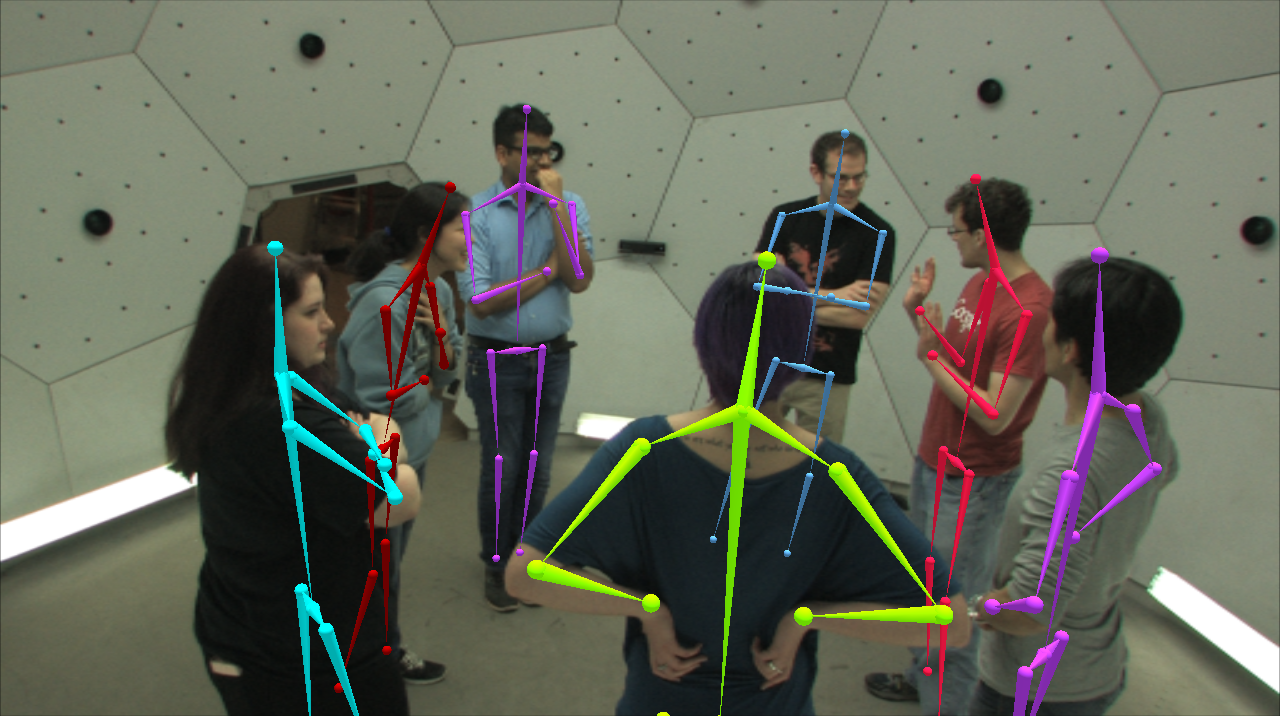
\includegraphics[width=0.245\textwidth]{figures/datasetEx/mafia}} 
%	\subfloat[Ultimatum]{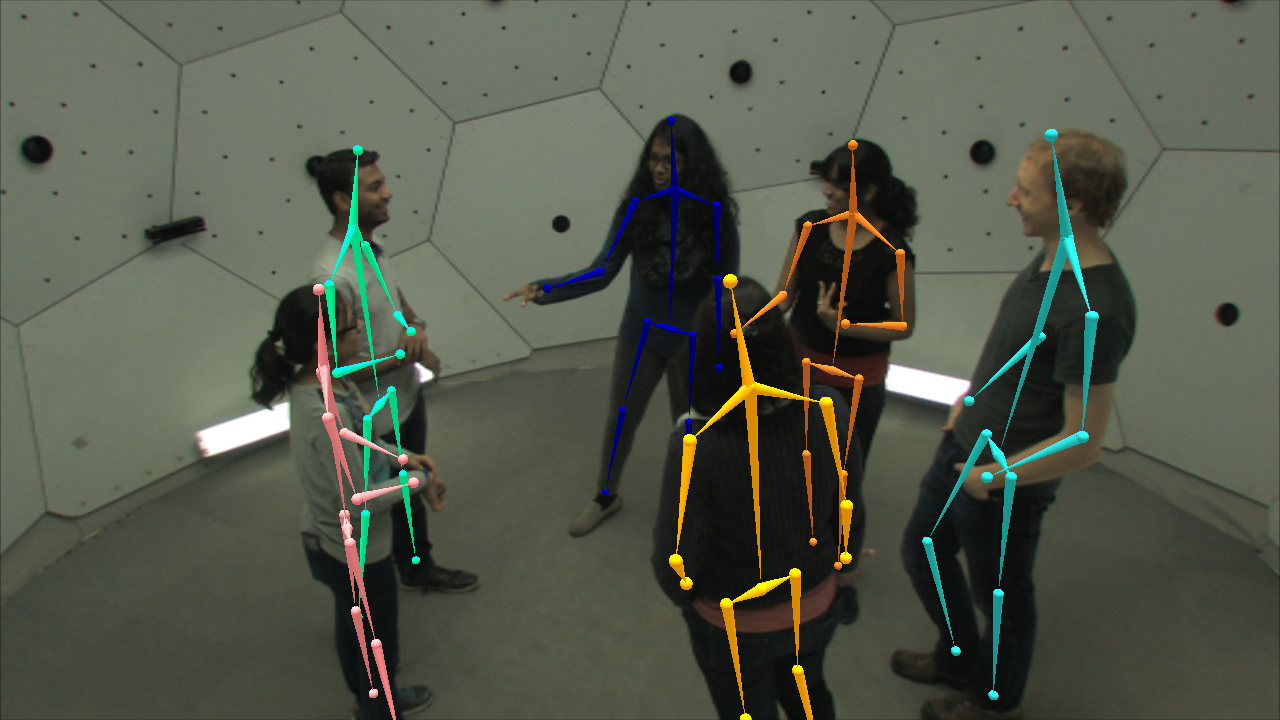
\includegraphics[width=0.245\textwidth]{figures/datasetEx/ultimatum}} 
%	\subfloat[Haggling]{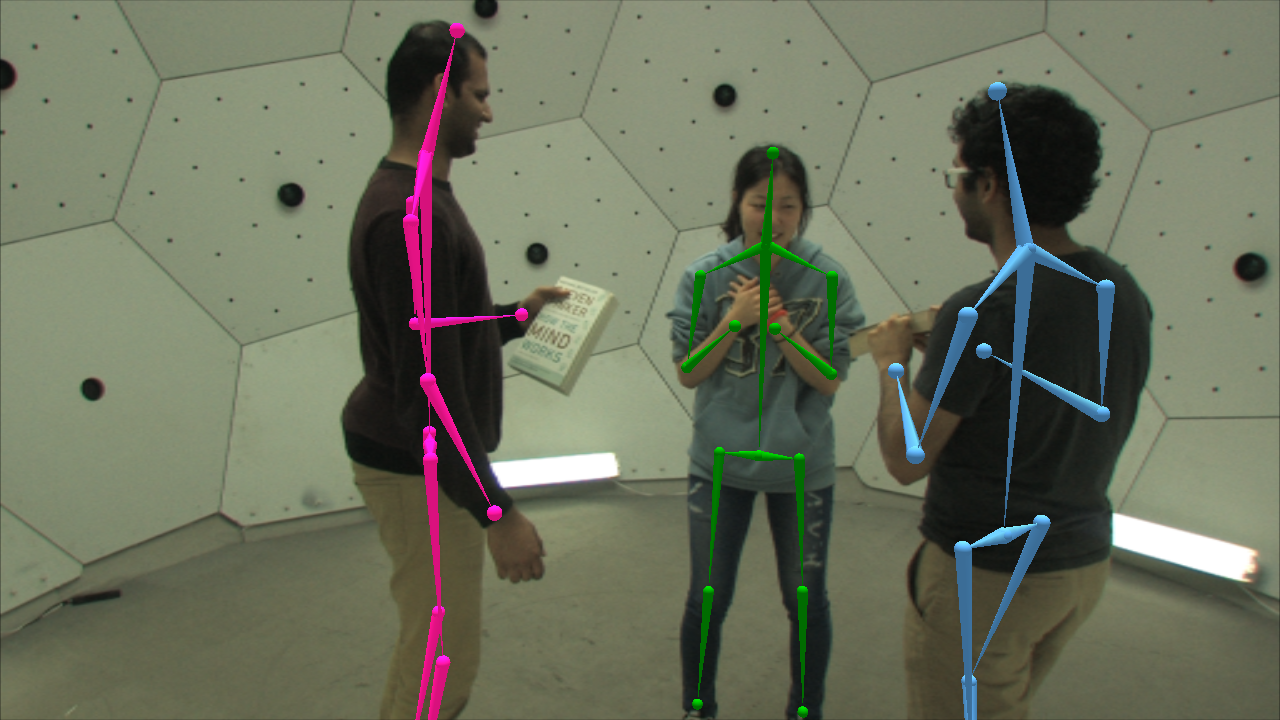
\includegraphics[width=0.245\textwidth]{figures/datasetEx/haggling}}   
%	\subfloat[007-Bang]{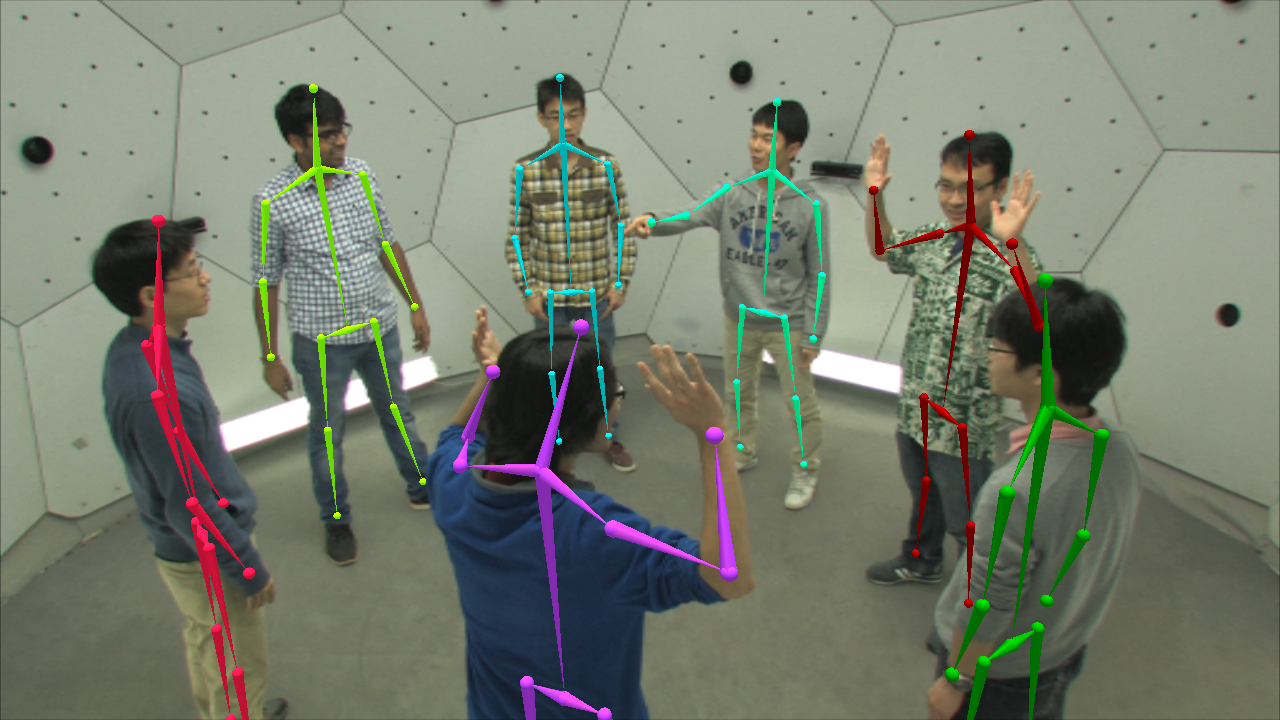
\includegraphics[width=0.245\textwidth]{figures/datasetEx/bang}}   
%	\caption{Example scenes of social game sequences. The reconstructed 3D skeletons from the 480 VGA views are projected on novel HD views.} 
%	\label{fig:socialGames}
%\end{figure}

\begin{figure}[t]
	\centering
	\begin{subfigure}{0.245\textwidth}
	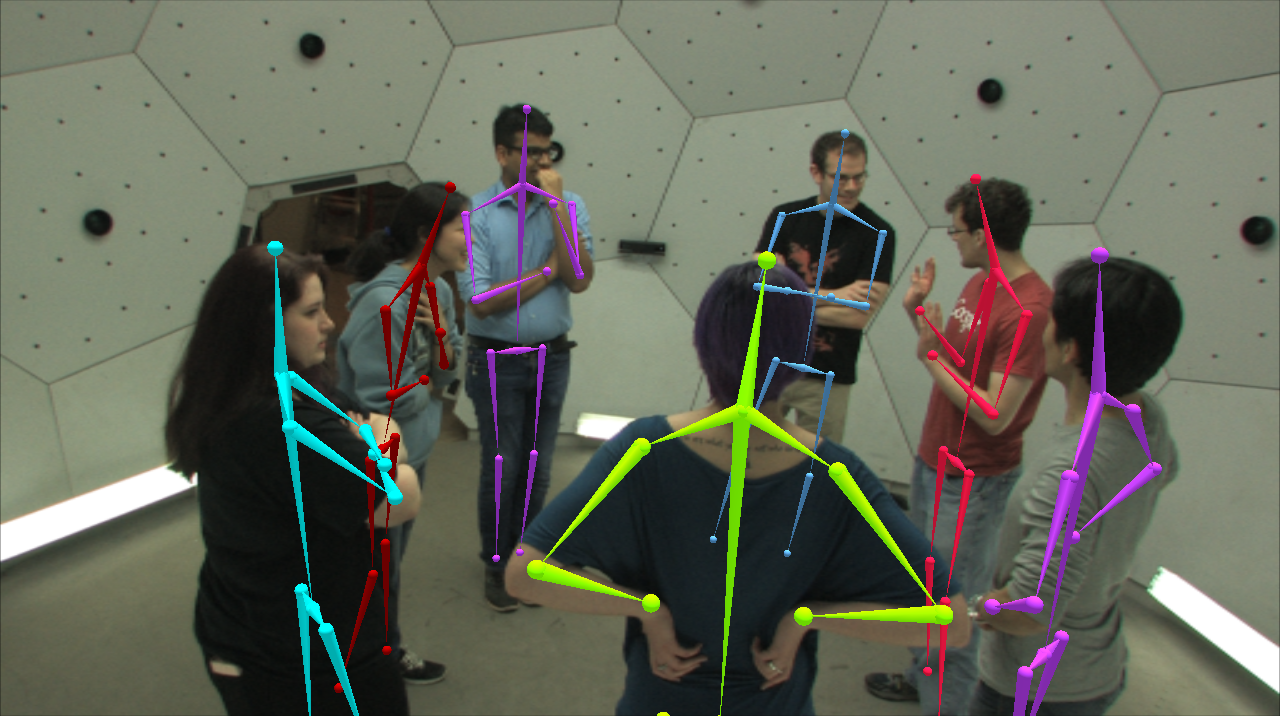
\includegraphics[width=\textwidth]{figures/datasetEx/mafia}
		\caption{Mafia}
	\end{subfigure}
	\begin{subfigure}{0.245\textwidth}
		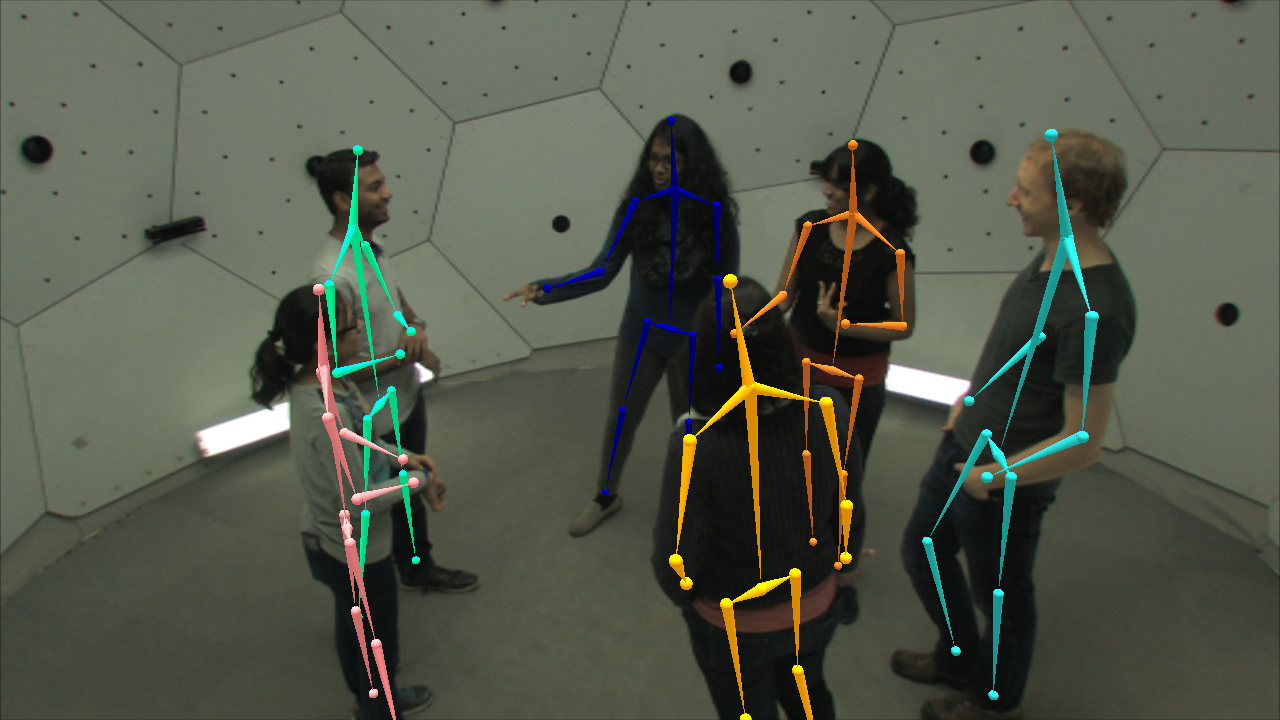
\includegraphics[width=\textwidth]{figures/datasetEx/ultimatum}
				\caption{Ultimatum}
	\end{subfigure}
	\begin{subfigure}{0.245\textwidth}

		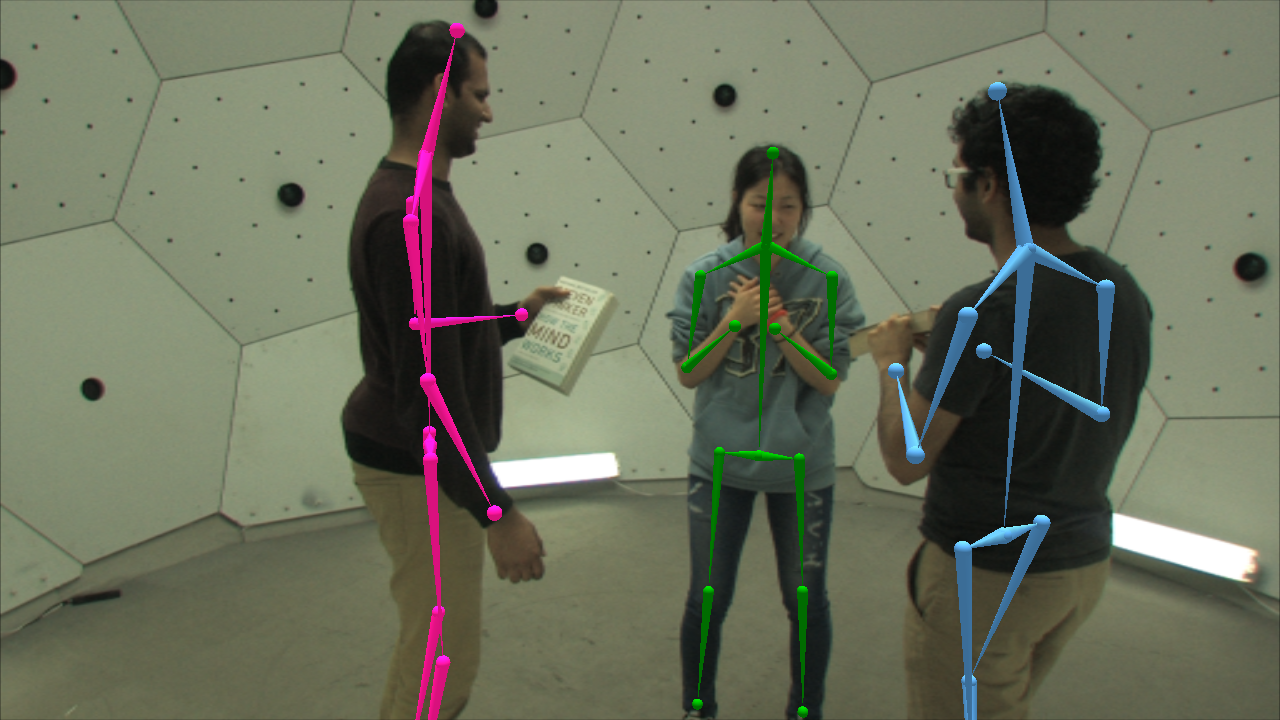
\includegraphics[width=\textwidth]{figures/datasetEx/haggling}
				\caption{Haggling}
	\end{subfigure}
	\begin{subfigure}{0.245\textwidth}

		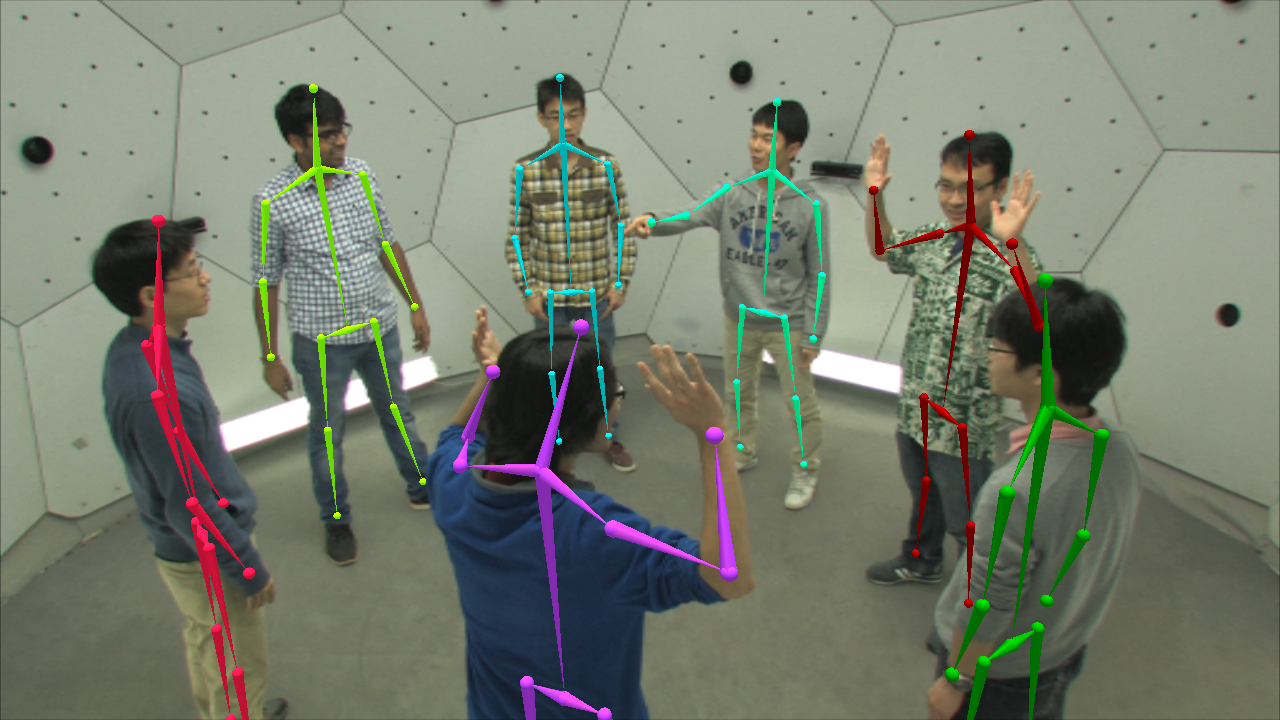
\includegraphics[width=\textwidth]{figures/datasetEx/bang}
				\caption{007-Bang}
	\end{subfigure}
	\caption{Example scenes of social game sequences. The reconstructed 3D skeletons from the 480 VGA views are projected on novel HD views.} 
	\label{fig:socialGames}
\end{figure}

%\subsection{Dataset and Capture Procedures}
%We captured a group of people engaged in social interactions using the Panoptic Studio\footnote{Some sequences were captured with fewer than the full set of cameras due to hardware failures during capture.}. To evoke natural interactions, we involved participants in various games: \emph{Ultimatum}, \emph{Mafia}, \emph{Haggling}, and \emph{007-Bang Game}. The first two games are used in experimental economics and psychology to study conflict and cooperation, and the latter two games also induce a variety of rich non-verbal signals in participants. Example scenes of each game are shown in Figure~\ref{fig:socialGames}. Refer to the supplementary material for descriptions of the games and capture procedures. In our captures, subjects were informed of the rules of the game but were otherwise not instructed about how to behave, nor was their clothing or appearance controlled. They were also not initially aware of our research goals to avoid potential biases in their gestures\footnote{The majority of the sequences are captured with people randomly recruited from a university campus; some sequences were captured for testing purposes and feature researchers with knowledge of the project. Those sequences are marked in our dataset website.}. The scenes in our dataset contain various natural motions which may commonly occur in the interactions of daily life, as shown in Figure~\ref{fig:iconicPoses} and \ref{fig:qualitativeSocial}. 
%% During the capture, people come in and out of the system. 
%
%To additionally demonstrate the performance of our system and methods, we capture other challenging sequences, including a group of 8 seated people participating in a discussion (\emph{meeting} sequence), a mother and a toddler at play (\emph{toddler} sequence), musical performances with severe occlusions due to the instruments (\emph{drummer} and \emph{cellist}), and a sequence featuring various fast motions and challenging postures (\emph{dancer}). 
%
%In aggregate, the dataset contains about 198 minutes ($\sim$297K frames) of videos, for a total of about 154 million images. Our dataset is summarized in the supplementary material. 
% 338 individuals, assuming the same person in different sessions is different, are participated for the study and about 1 M of 3D poses are reconstructed. 
%
%The main distinguishing features of this collection compared to previous markerless motion capture datasets are: (1) natural interactions in the scenes showing rich and subtle non-verbal cues, (2) social groups of up to 8 interacting people, and (3) coverage by a large number of views (up to 521). We make all the data available on our website, including all synchronized camera feeds, calibration, 3D pose reconstruction results, and 3D trajectory streams: \url{https://domedb.perception.cs.cmu.edu}. %\url{https://domedb.perception.cs.cmu.edu}.
%
%\begin{figure}[t]
%	\centering
%	\captionsetup{position=top}
%	\subfloat[Two people]{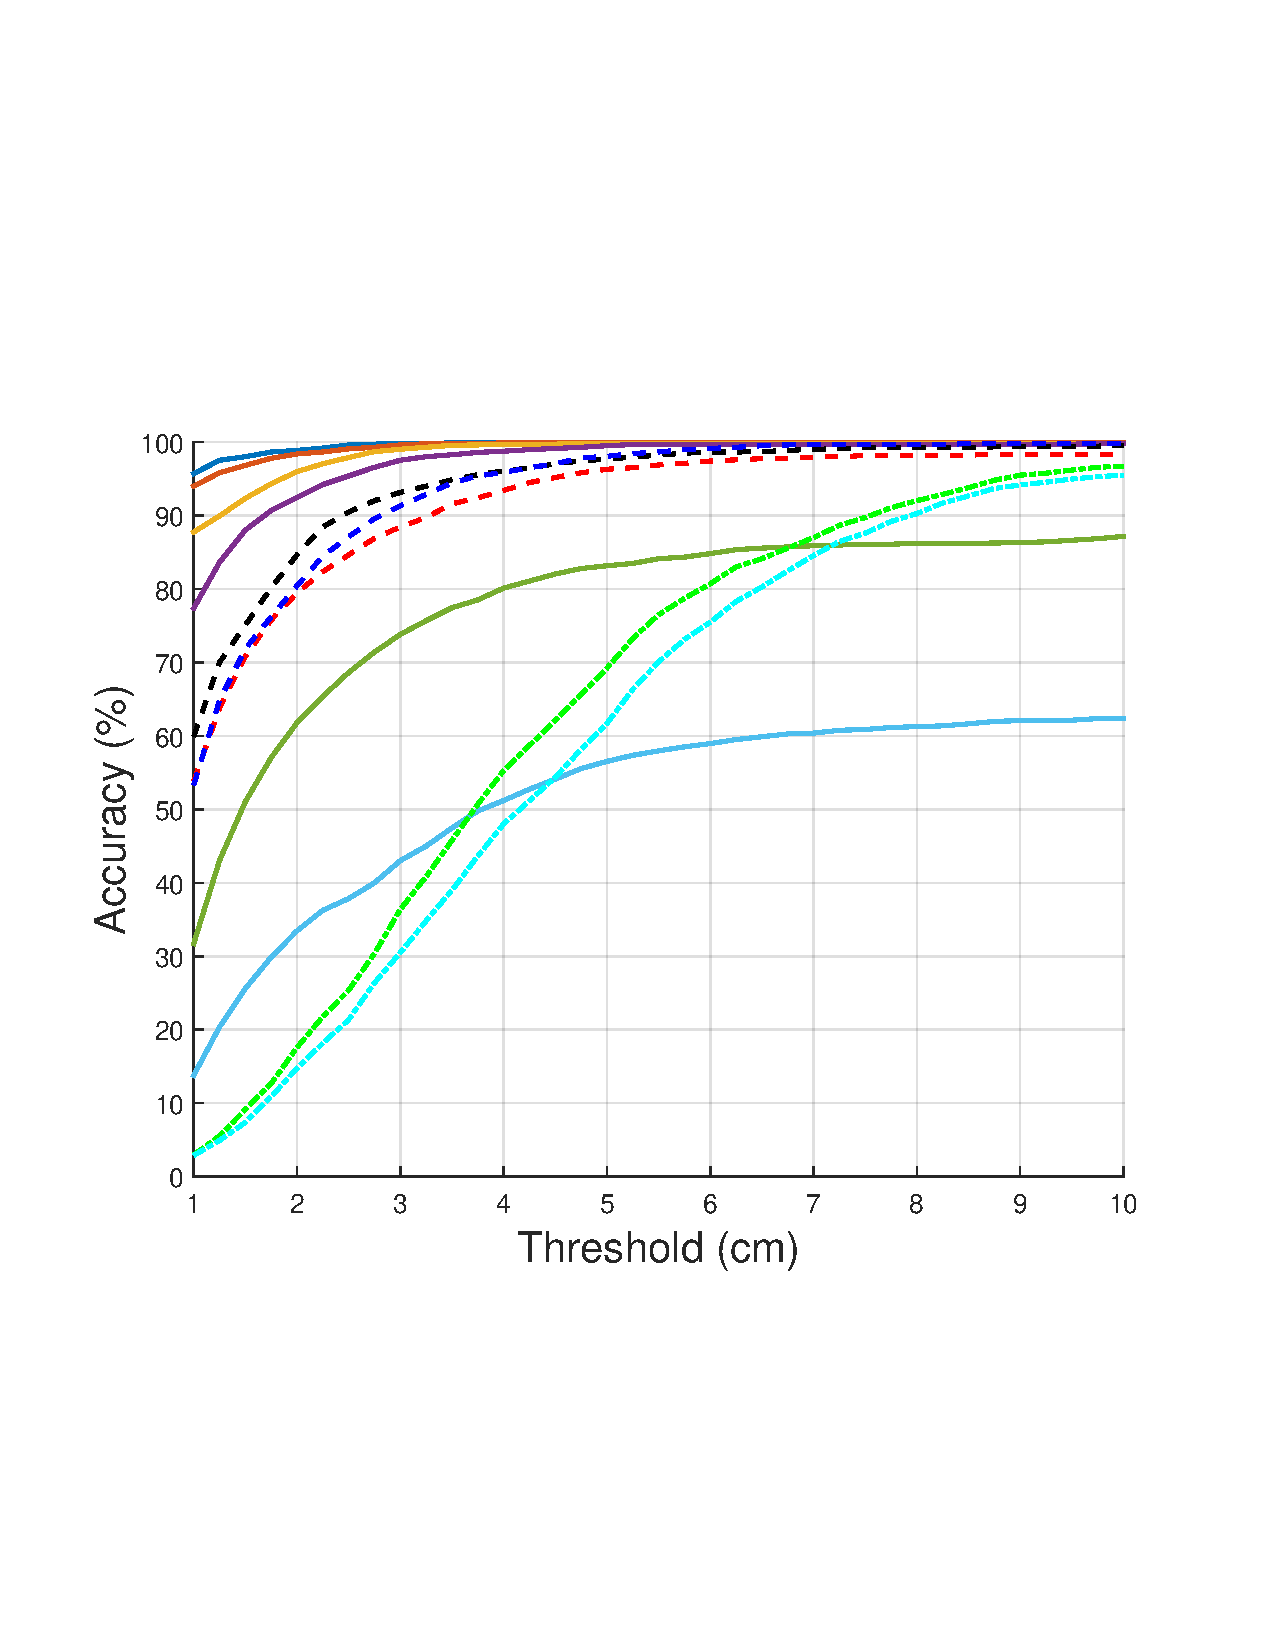
\includegraphics[trim=40 180 60 170,clip,width=0.245\textwidth]{figures/0822_quant_noLegend/PCK-Threshold-two-people.pdf}
%		\llap
%		{\shortstack{%
%				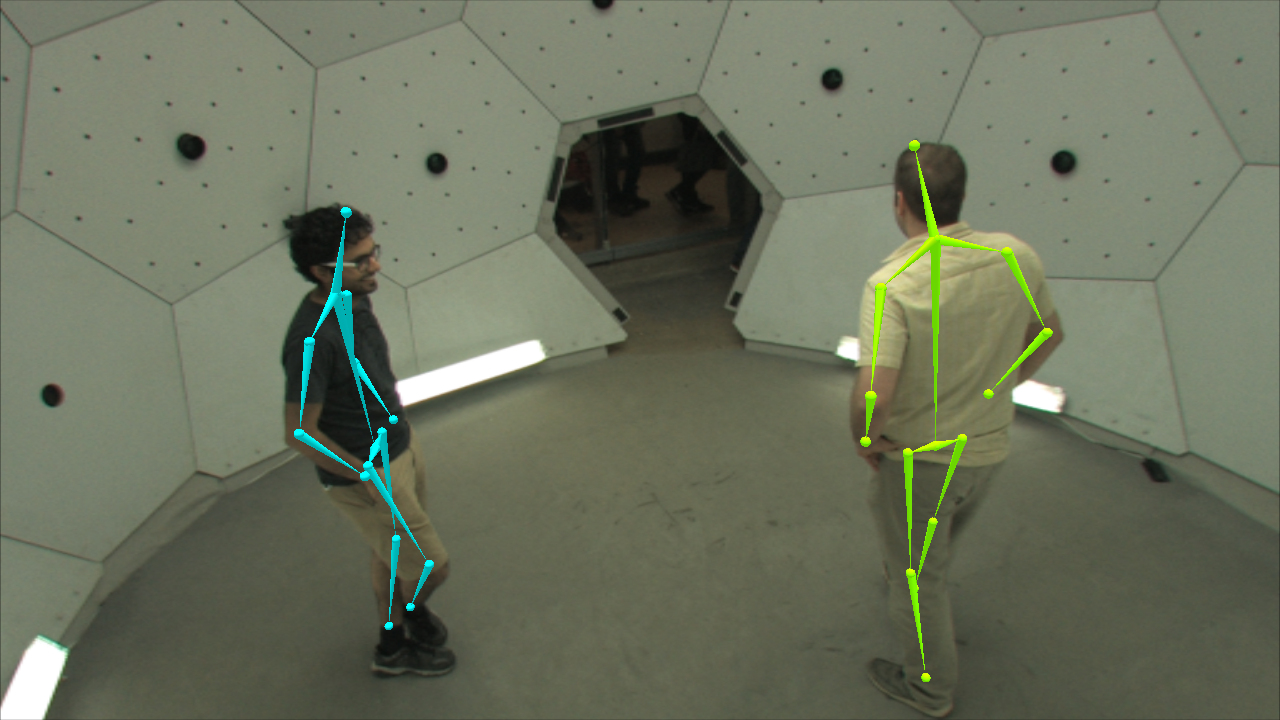
\includegraphics[width=0.1\textwidth]{figures/0807_quant_noLegend/two}\\
%				\rule{0ex}{3ex}	%vertical
%			}
%			\rule{1ex}{0ex}	%horizontal
%		}	
%	}
%	\subfloat[Three people]{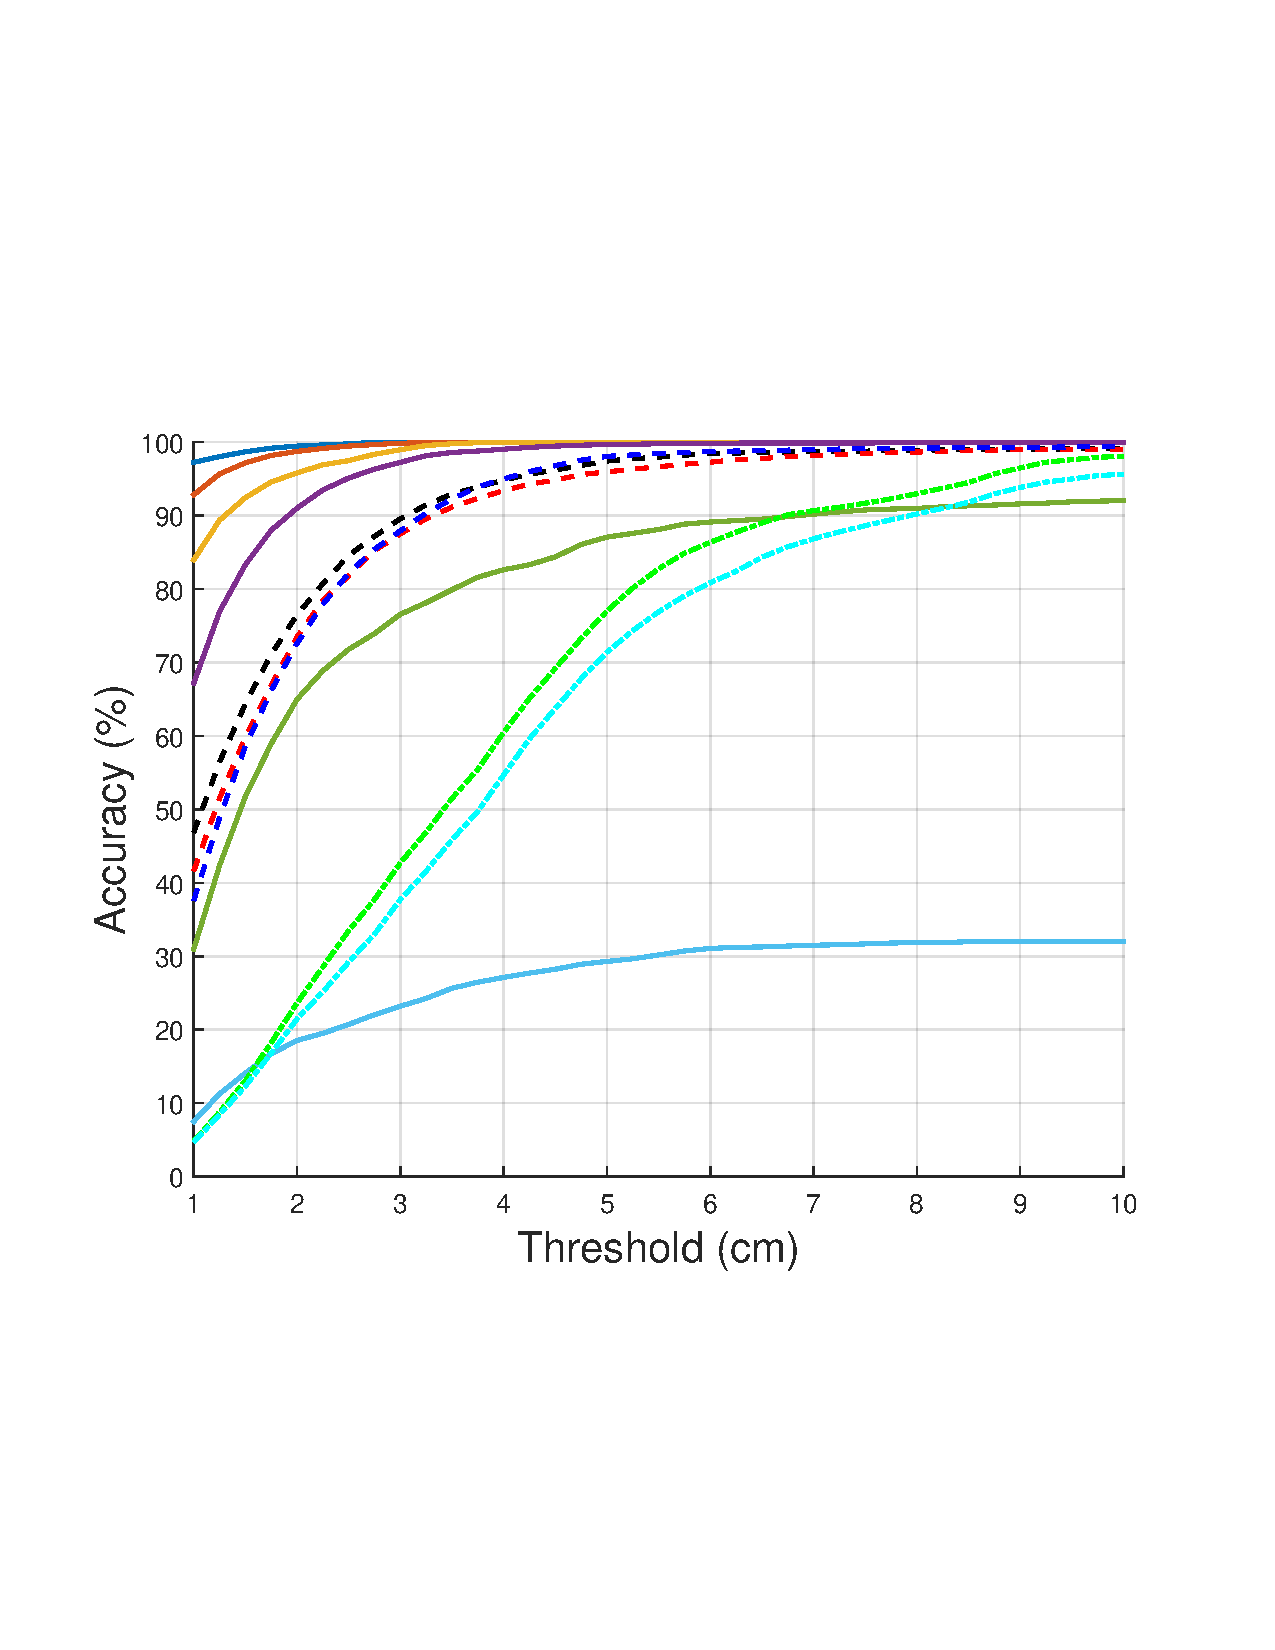
\includegraphics[trim=40 180 60 170,clip,width=0.245\textwidth]{figures/0822_quant_noLegend/PCK-Threshold-three-people.pdf}
%		\llap
%		{\shortstack{%
%				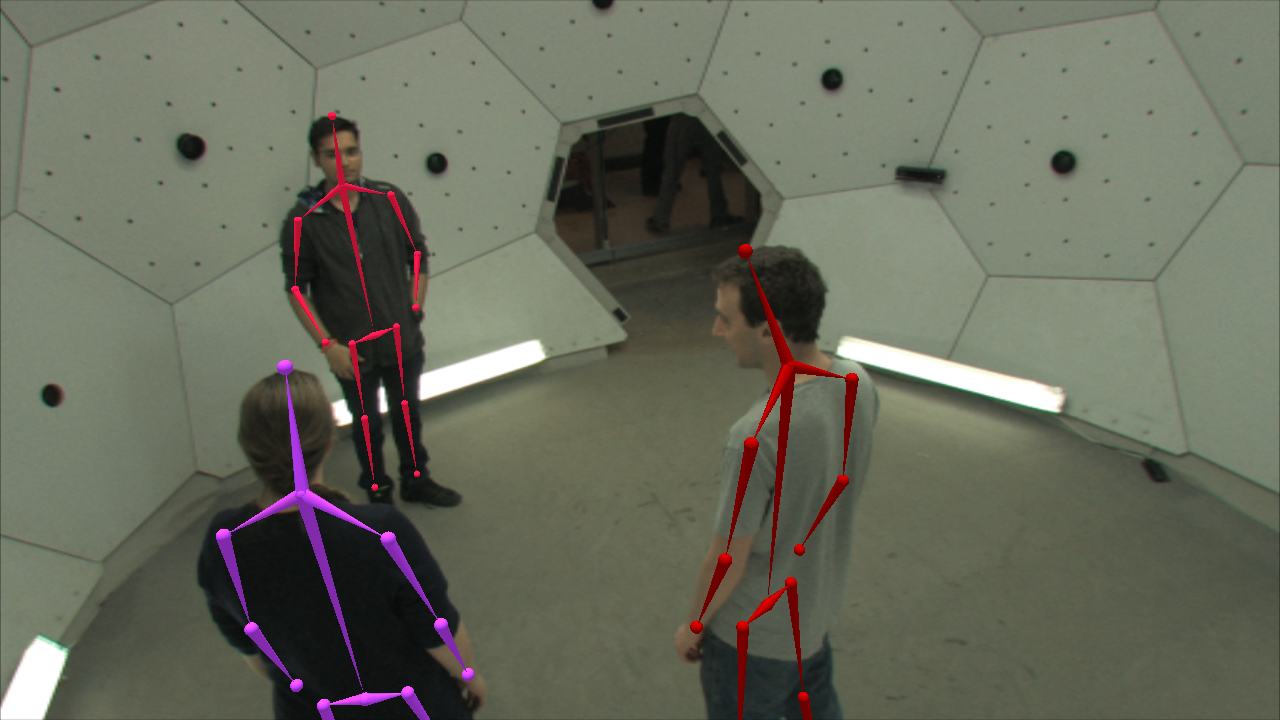
\includegraphics[width=0.1\textwidth]{figures/0807_quant_noLegend/three}\\
%				\rule{0ex}{3ex}
%			}
%			\rule{1ex}{0ex}
%		}	
%	}
%	\subfloat[Five people]{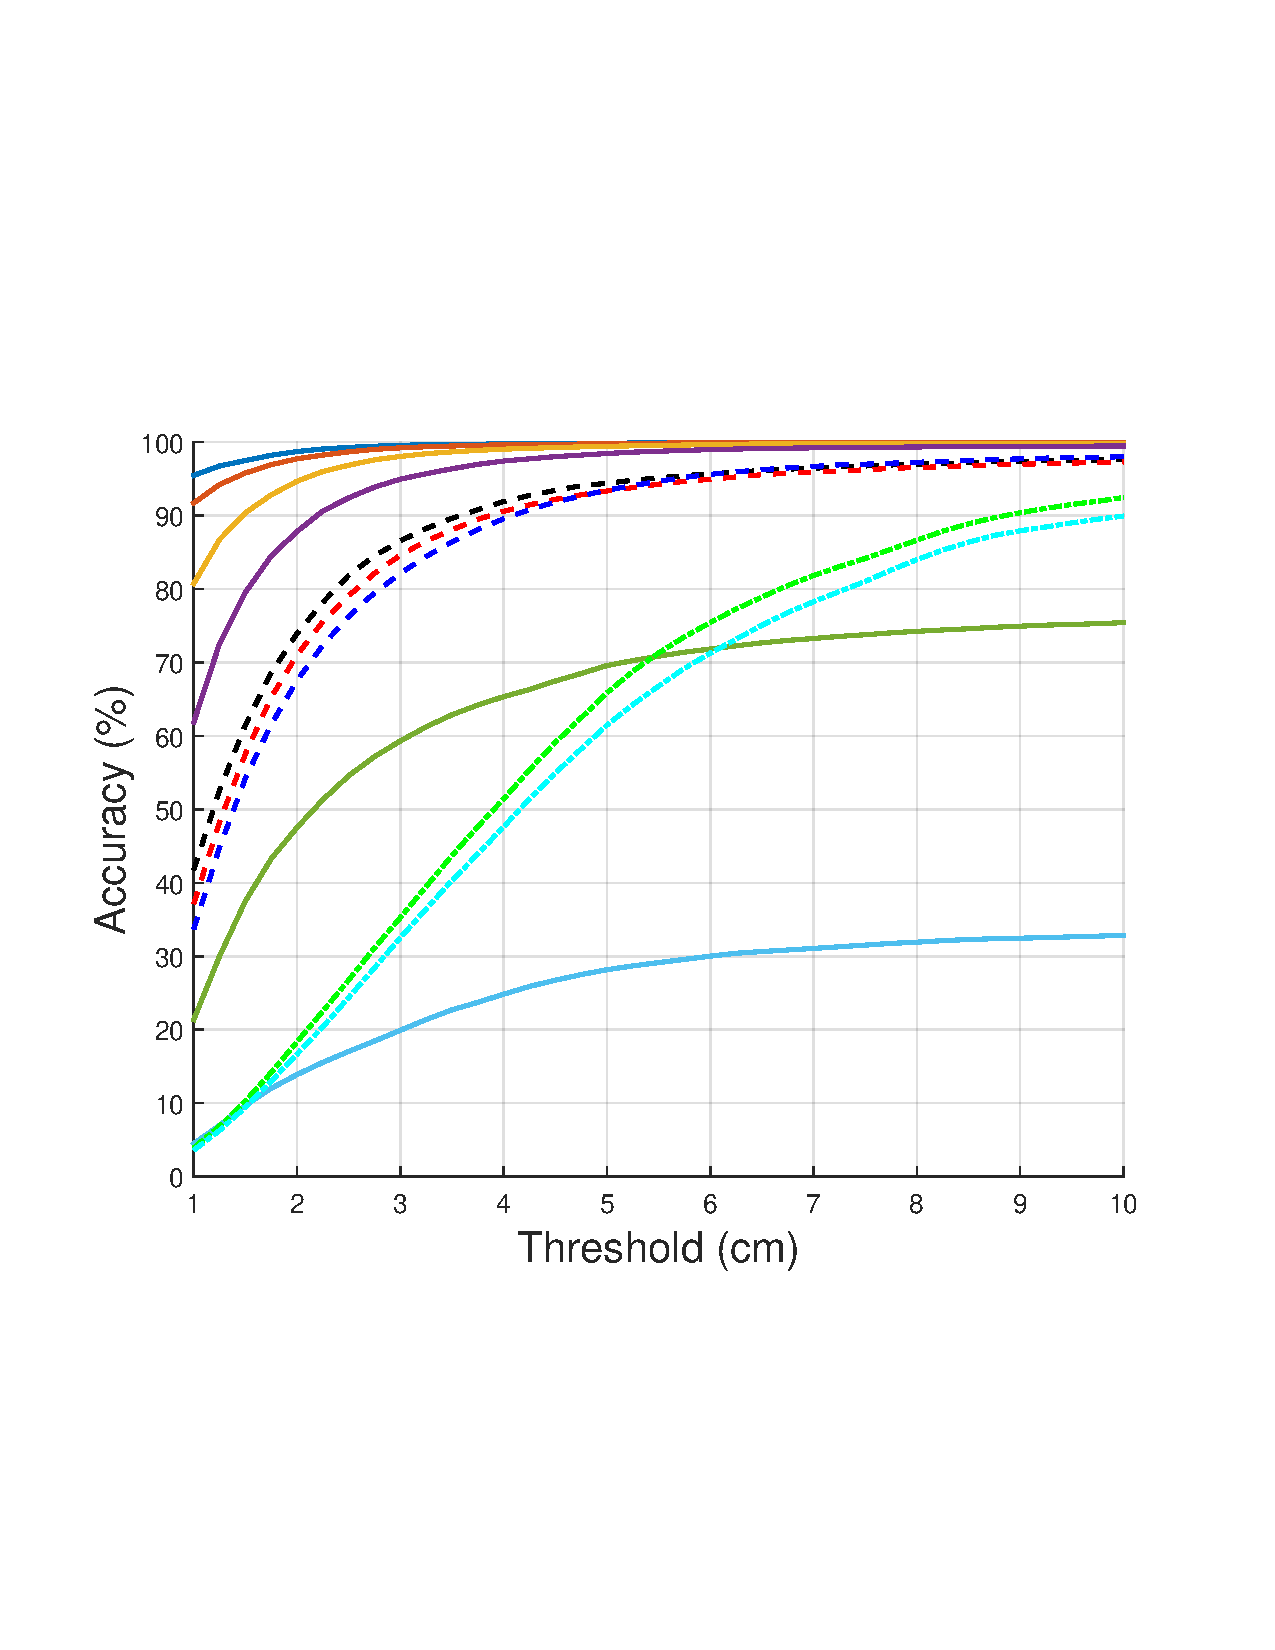
\includegraphics[trim=40 180 60 170,clip,width=0.245\textwidth]{figures/0822_quant_noLegend/PCK-Threshold-five-people.pdf}
%		\llap
%		{\shortstack{%
%				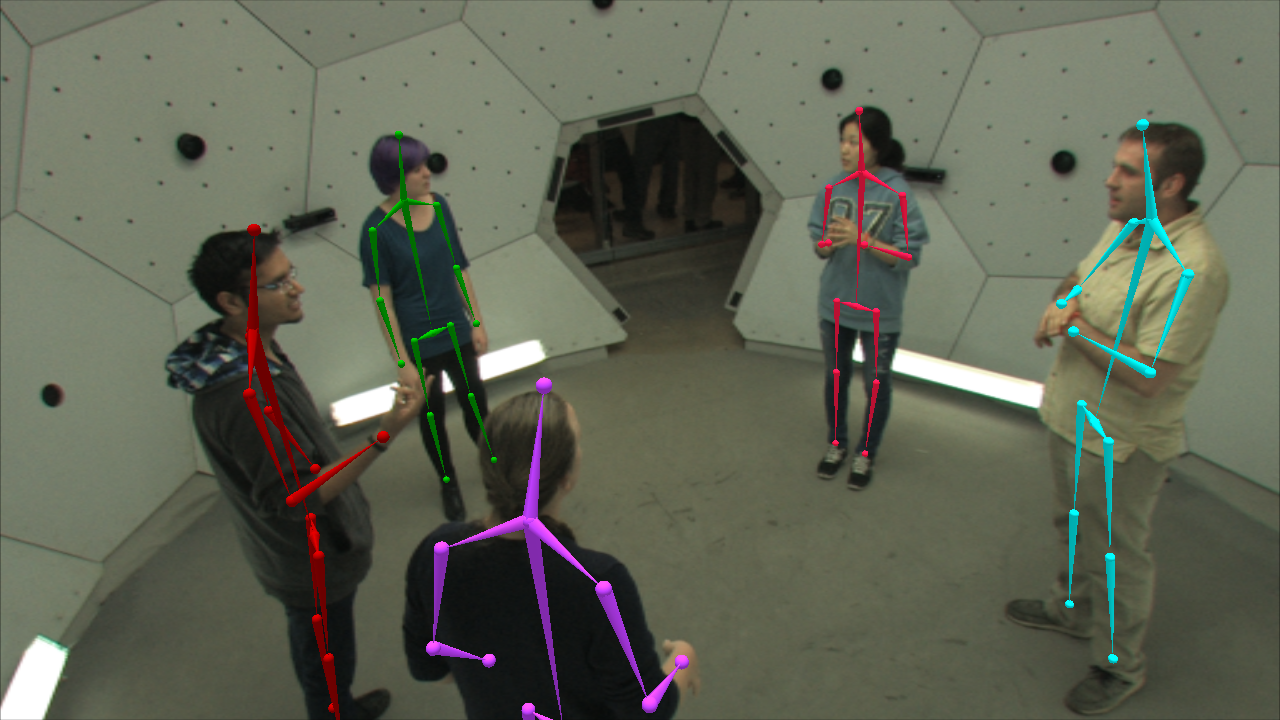
\includegraphics[width=0.1\textwidth]{figures/0807_quant_noLegend/five}\\
%				\rule{0ex}{3ex}
%			}
%			\rule{1ex}{0ex}
%		}	
%	}
%	\subfloat[Seven people]{\includegraphics[trim=40 180 60 170,clip,width=0.245\textwidth]{figures/0822_quant_noLegend/PCK-Threshold-seven-people.pdf}
%		\llap
%		{\shortstack{%
%				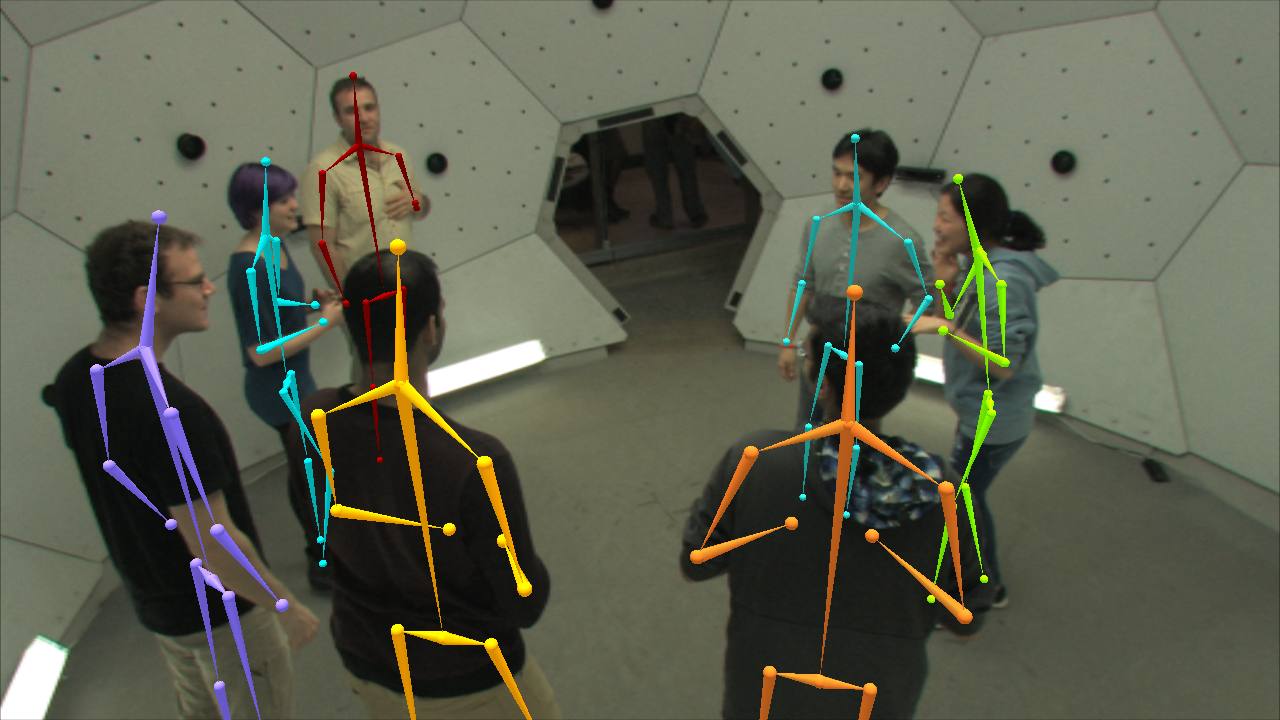
\includegraphics[width=0.1\textwidth]{figures/0807_quant_noLegend/seven}\\
%				\rule{0ex}{3ex}
%			}
%			\rule{1ex}{0ex}
%		}	
%	}\\
%	\subfloat{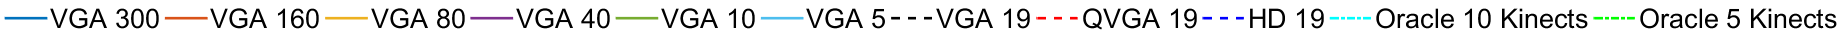
\includegraphics[width=0.9\textwidth]{figures/0822_quant_noLegend/legend}} 
%	\caption{Performance evaluation using Probability of Correct Keypoint (PCK) metric for varying number and type of cameras on \emph{160422 ultimatum1}. We use the result of 480 VGA cameras after manually excluding outliers as ground truth. The X-axis of each graph represents thresholds, and the Y-axis represents accuracy by the thresholds. Each graph is generated for scenes with a different number of people. The results demonstrate that more views (rather than higher resolution) are beneficial to improve accuracy, and the distinction is more noticeable if the scene contains more people.} 
%	\label{fig:quant1}
%\end{figure}



\begin{figure}[t]
	\centering
	\captionsetup{position=top}
	\begin{subfigure}{\textwidth}
		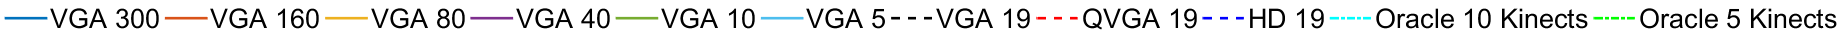
\includegraphics[width=\textwidth]{figures/0822_quant_noLegend/legend}
	\end{subfigure}\\
	\begin{subfigure}{0.245\textwidth}

		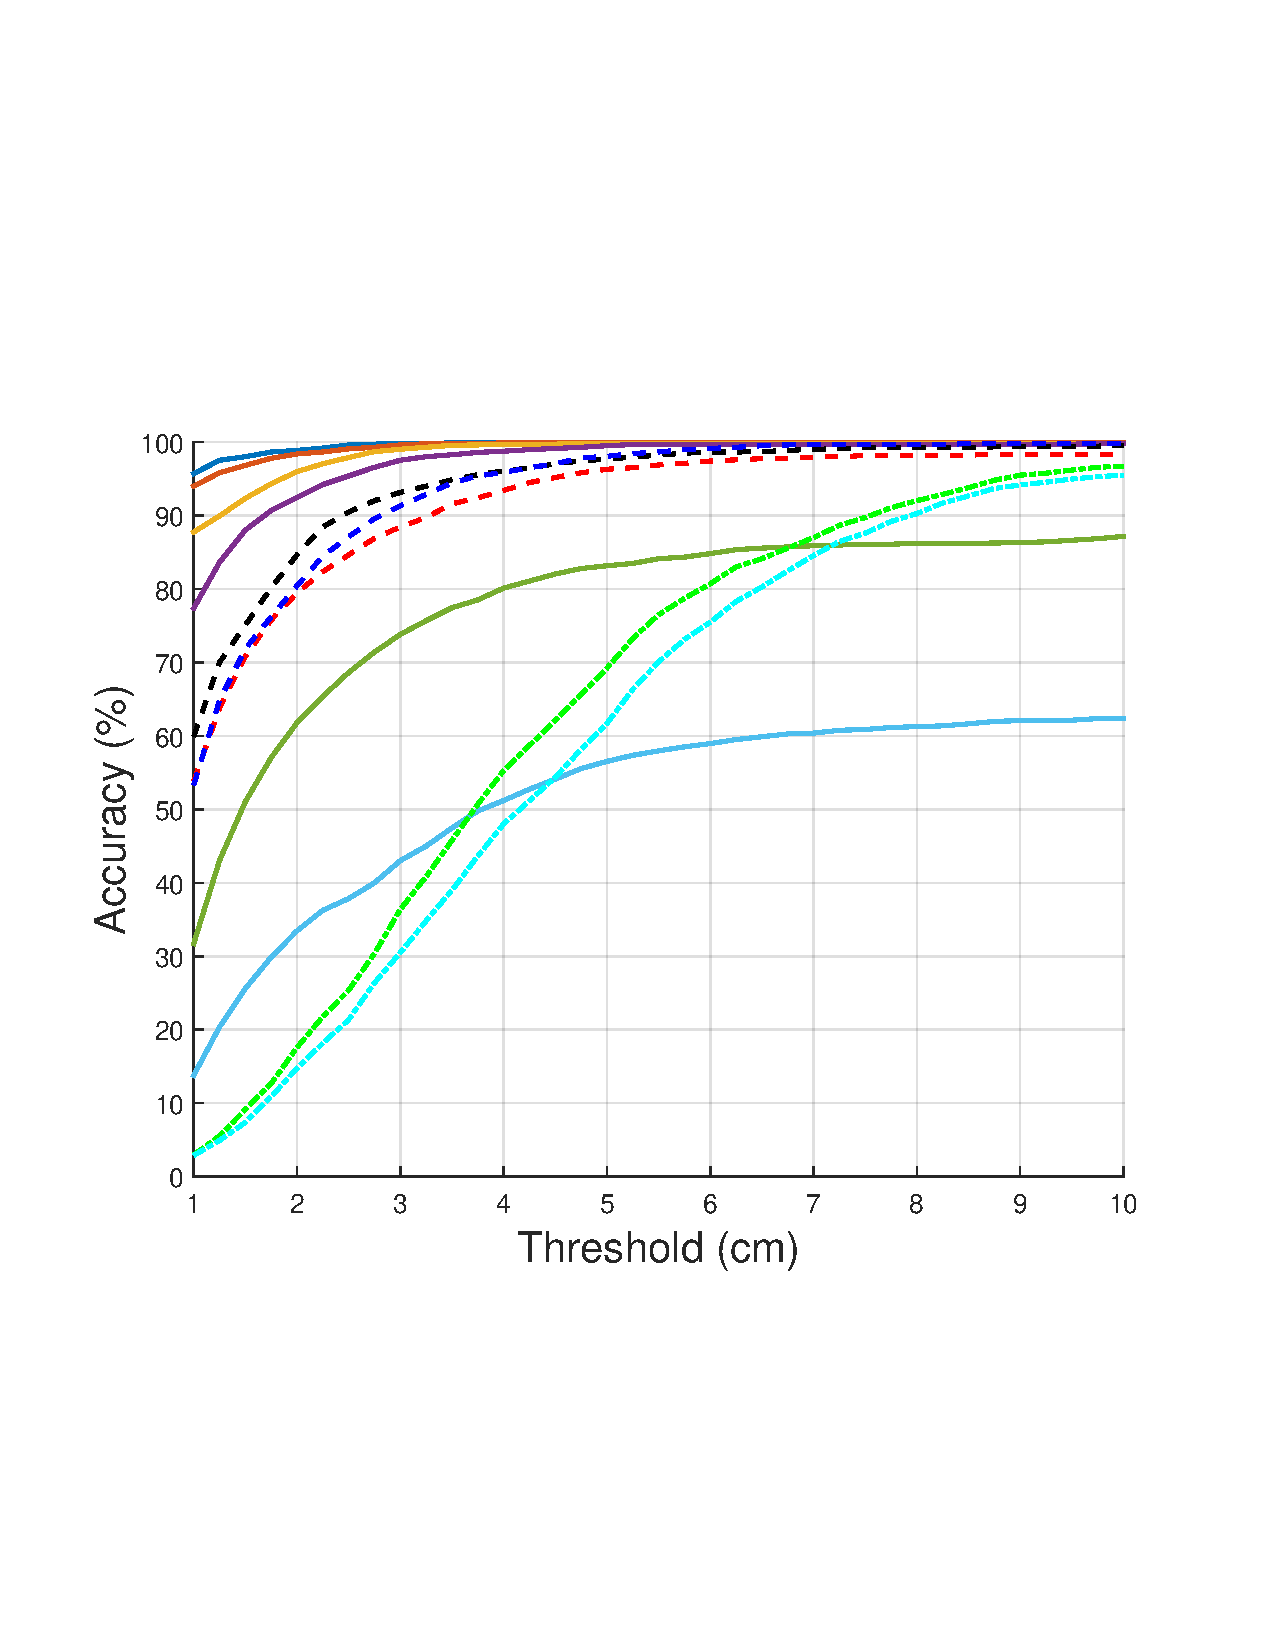
\includegraphics[trim=40 180 60 		170,clip,width=\textwidth]{figures/0822_quant_noLegend/PCK-Threshold-two-people.pdf}
%		\caption{Two people}		
	\end{subfigure}
	\begin{subfigure}{0.245\textwidth}

		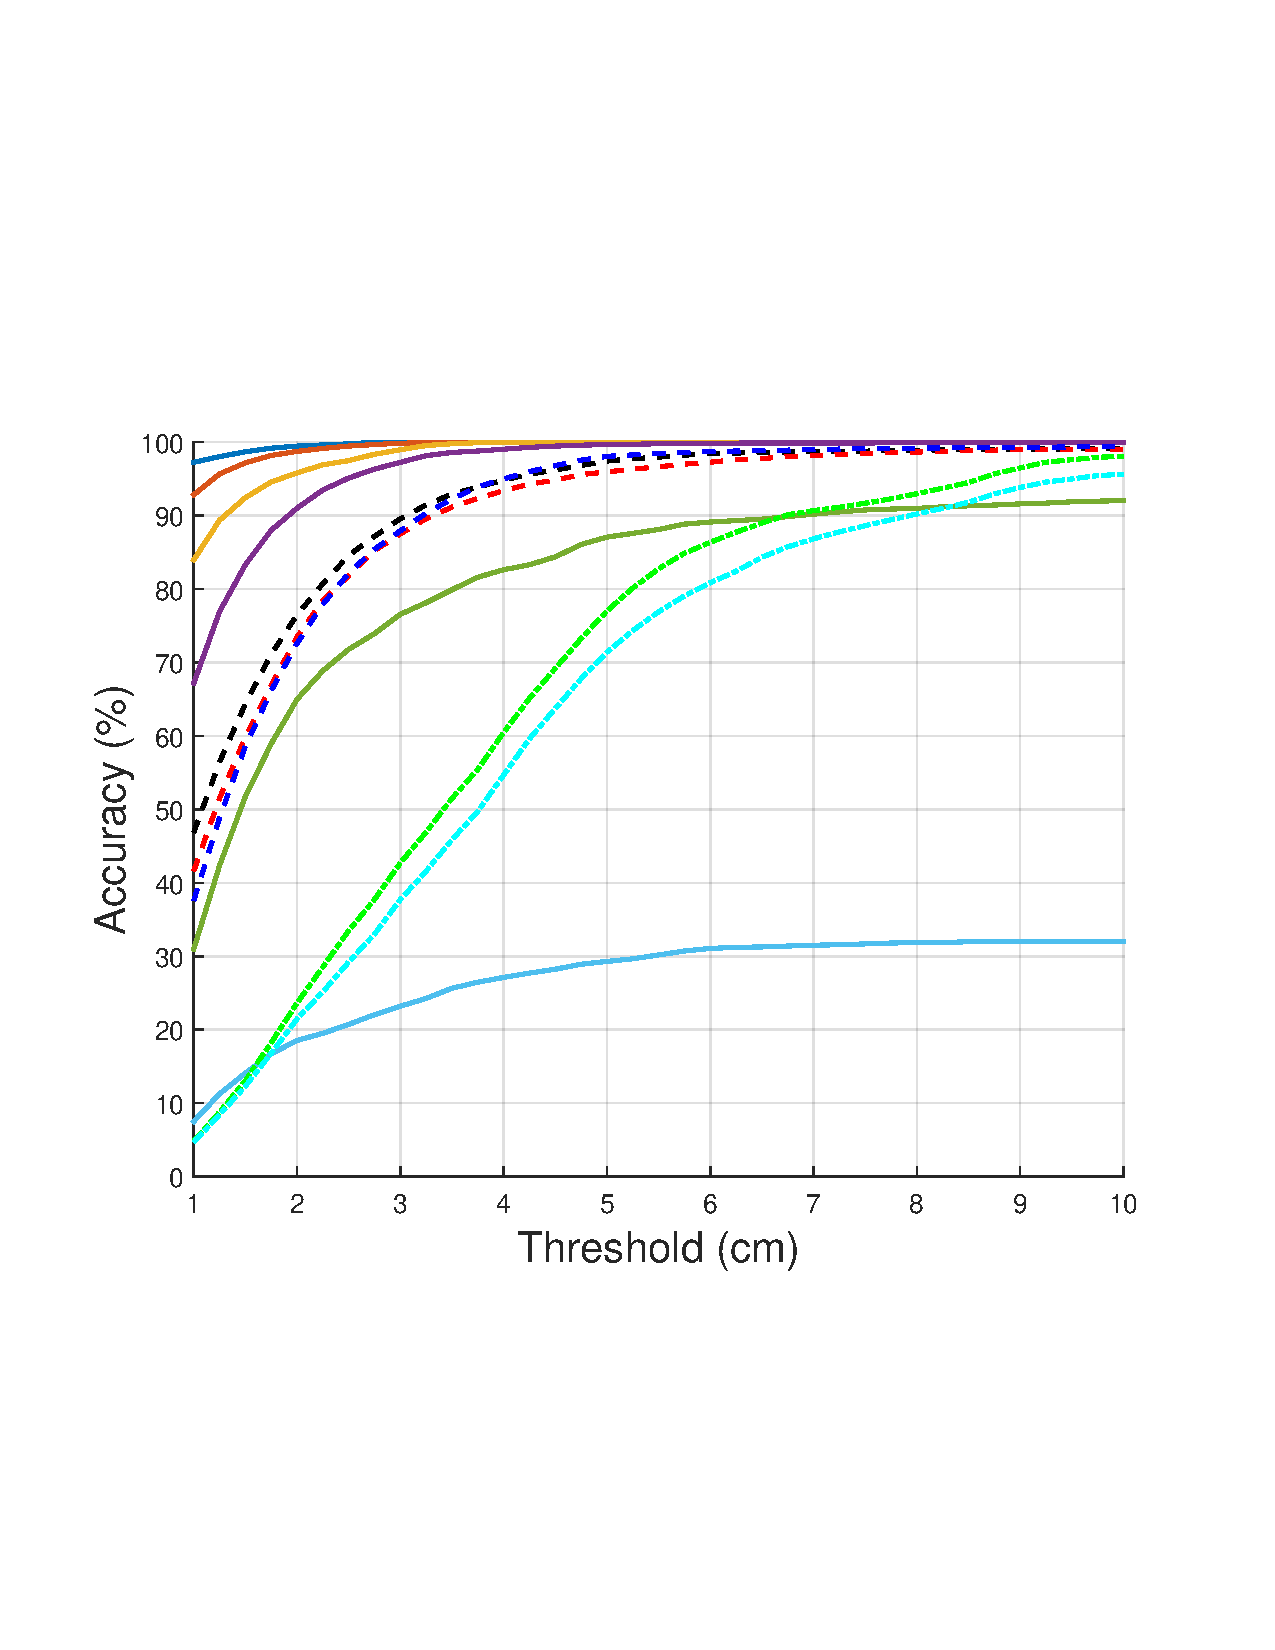
\includegraphics[trim=40 180 60 		170,clip,width=\textwidth]{figures/0822_quant_noLegend/PCK-Threshold-three-people.pdf}
		%\caption{Three  people}
	\end{subfigure}
	\begin{subfigure}{0.245\textwidth}

		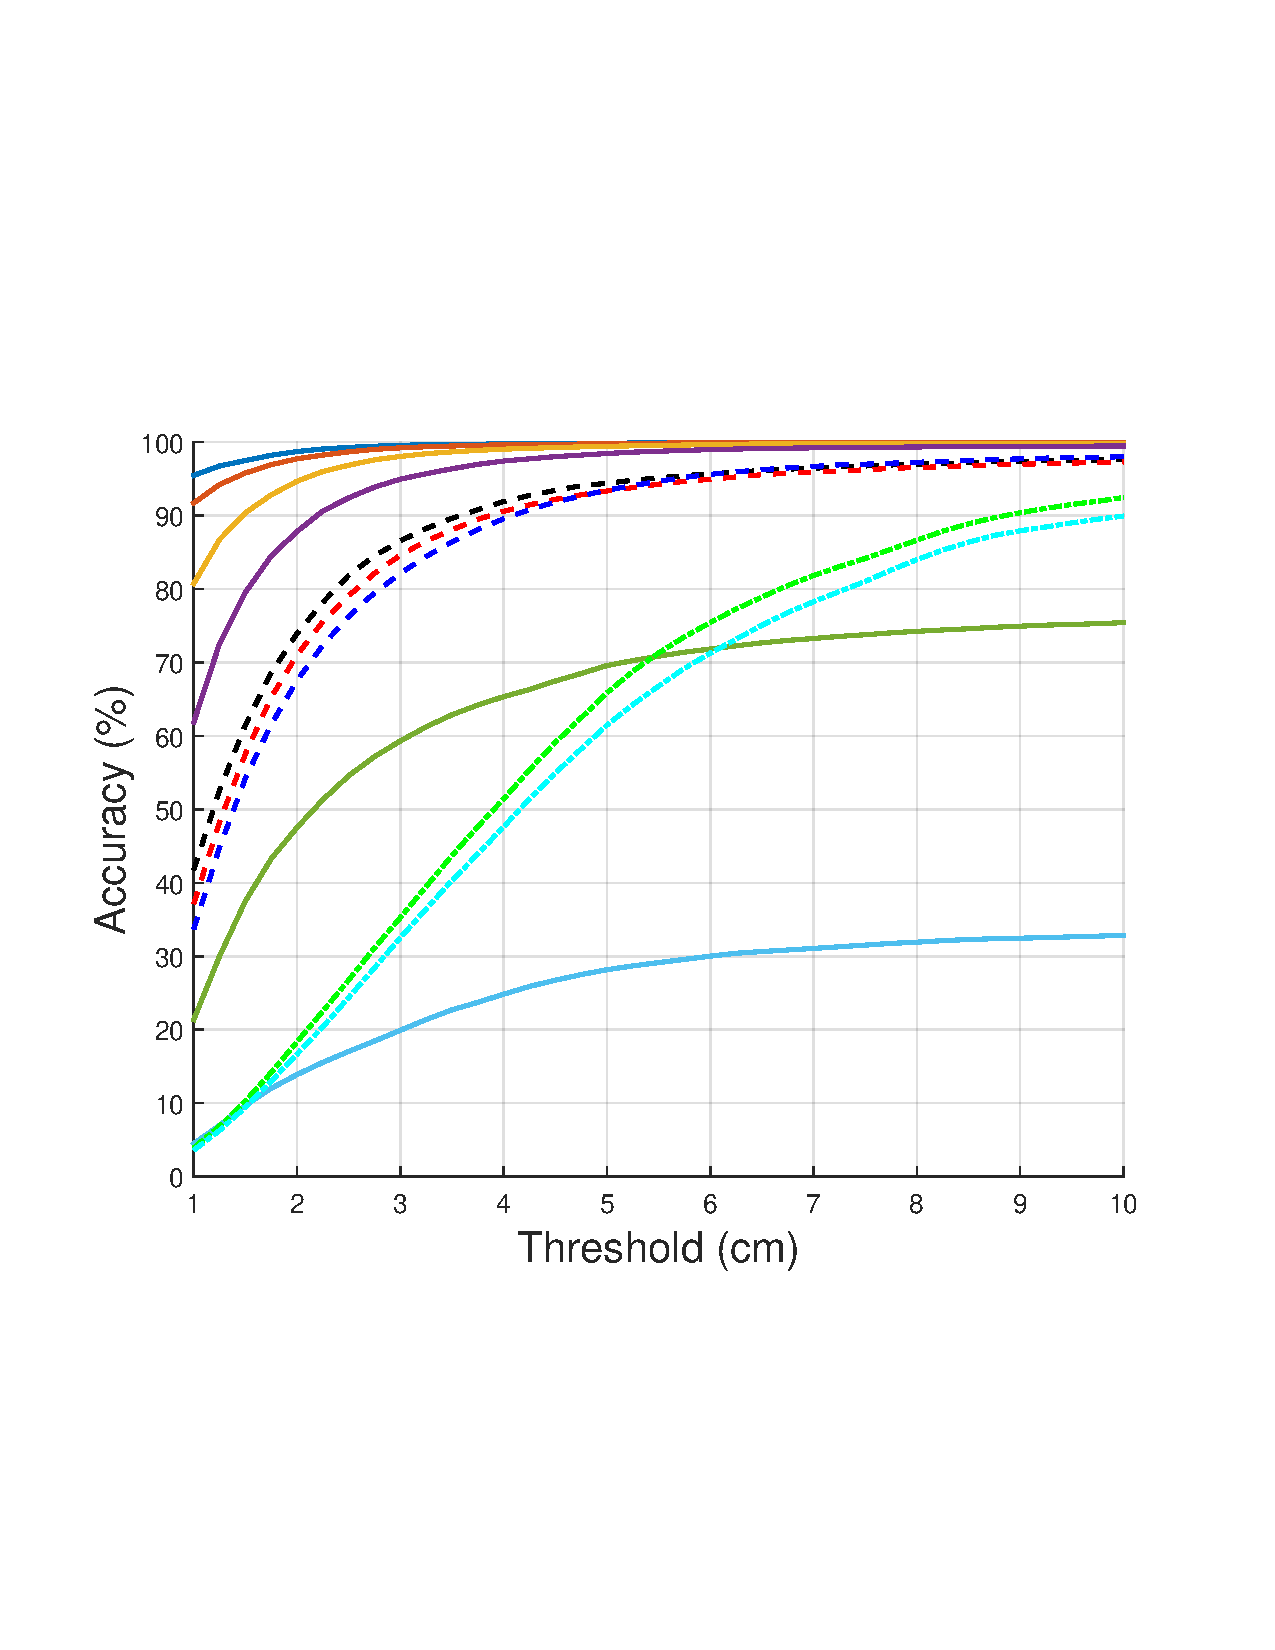
\includegraphics[trim=40 180 60 		170,clip,width=\textwidth]{figures/0822_quant_noLegend/PCK-Threshold-five-people.pdf}
		%\caption{Five people}
	\end{subfigure}
	\begin{subfigure}{0.245\textwidth}

		\includegraphics[trim=40 180 60 		170,clip,width=\textwidth]{figures/0822_quant_noLegend/PCK-Threshold-seven-people.pdf}
%		\caption{Seven people}
	\end{subfigure}\\
		\begin{subfigure}{0.245\textwidth}
			
			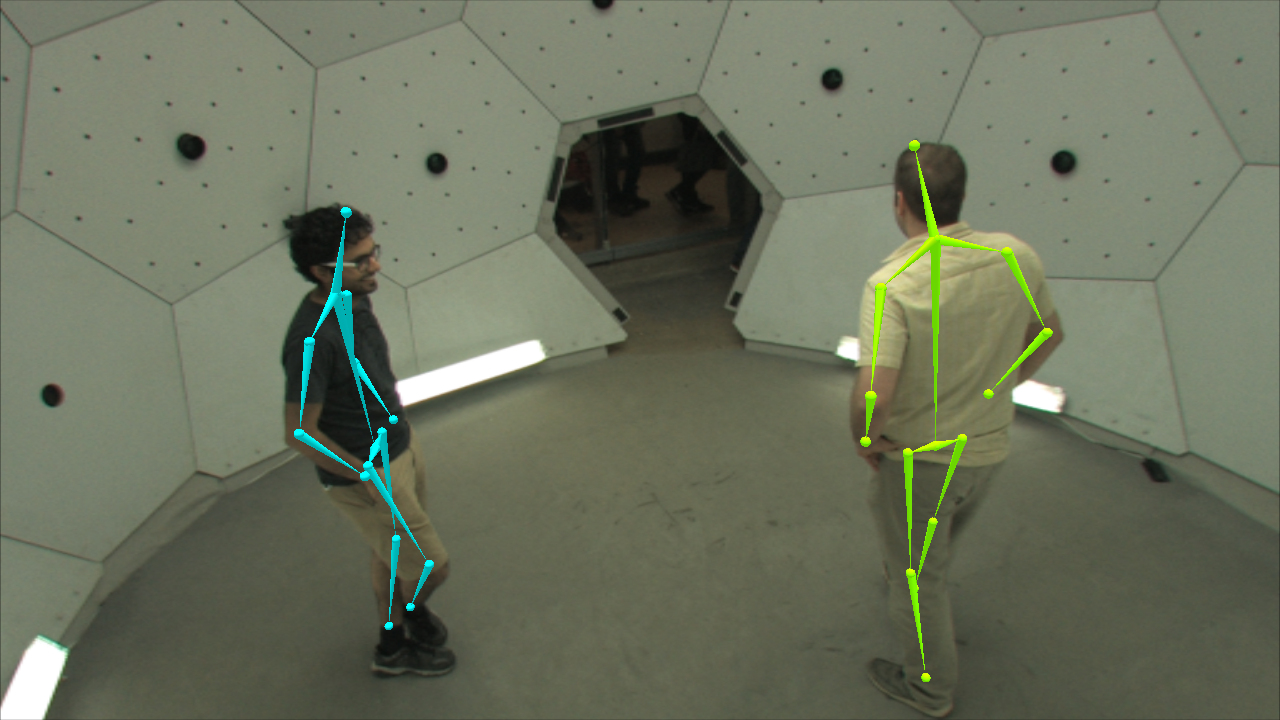
\includegraphics[width=\textwidth]{figures/0807_quant_noLegend/two}
	\caption{Two people}		
		\end{subfigure}
		\begin{subfigure}{0.245\textwidth}
			
			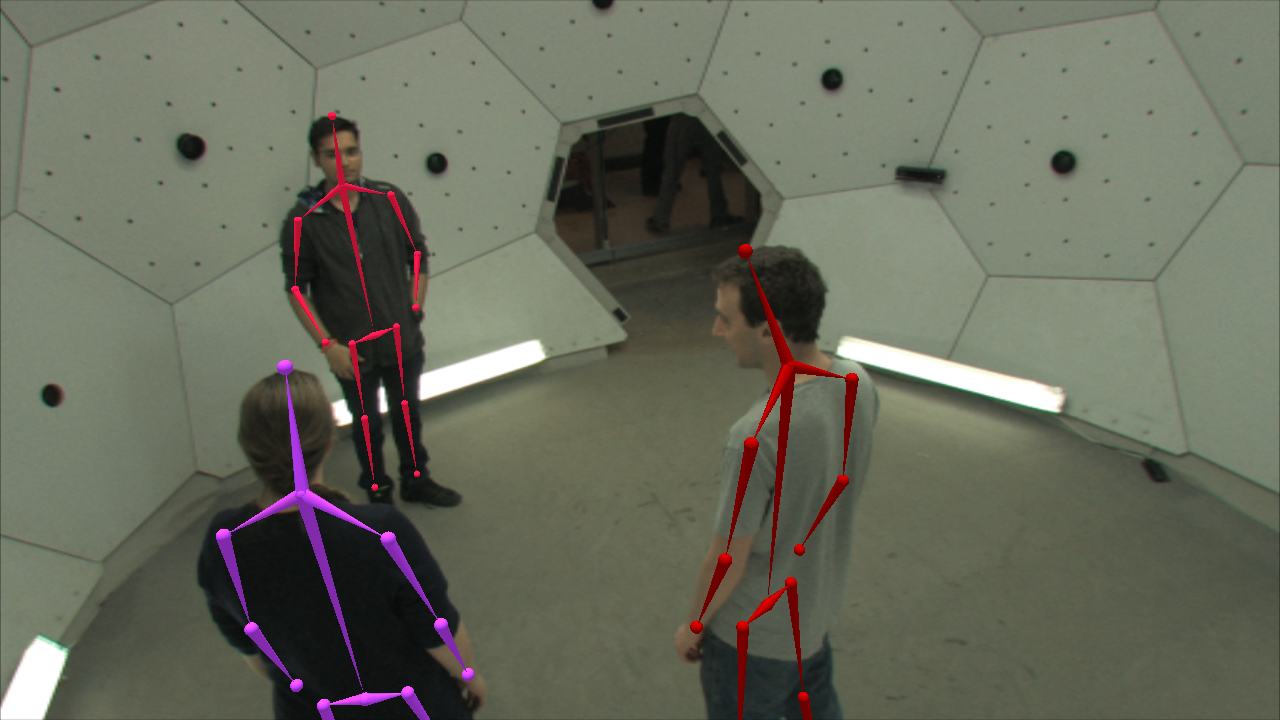
\includegraphics[width=\textwidth]{figures/0807_quant_noLegend/three}
	\caption{Three people}		
		\end{subfigure}
		\begin{subfigure}{0.245\textwidth}
			
			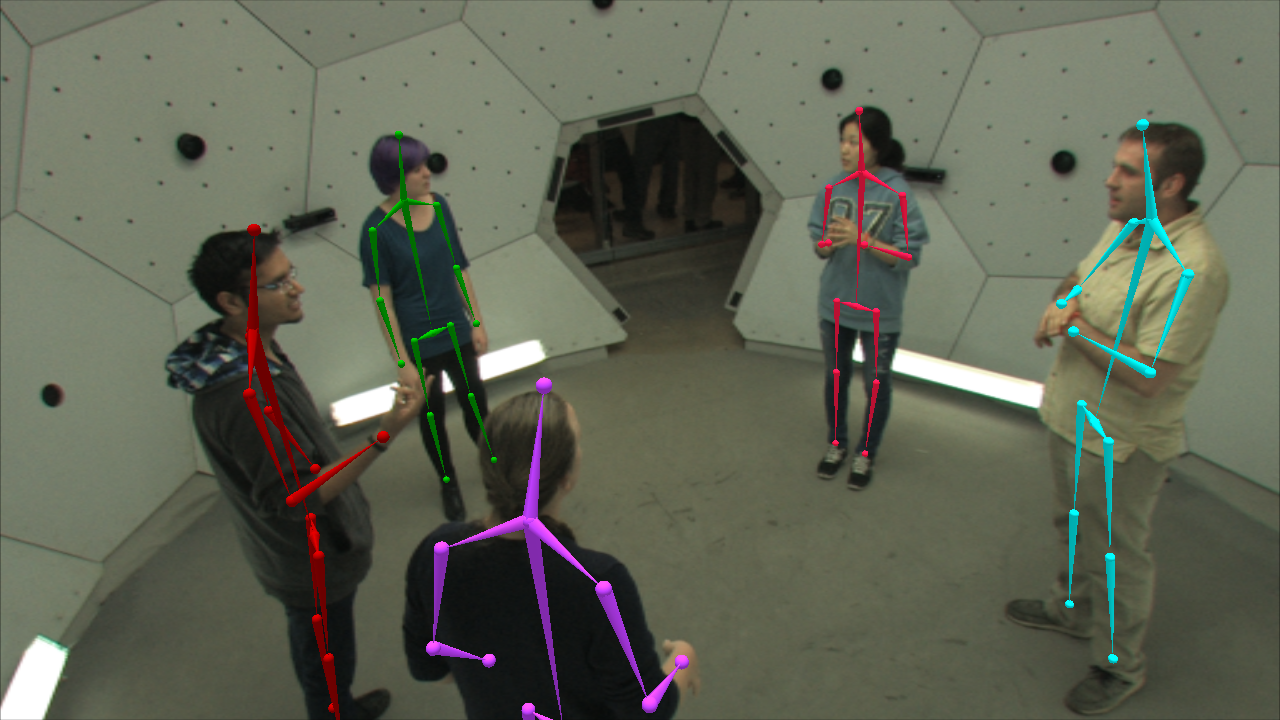
\includegraphics[width=\textwidth]{figures/0807_quant_noLegend/five}
	\caption{Five people}		
		\end{subfigure}
		\begin{subfigure}{0.245\textwidth}
			
			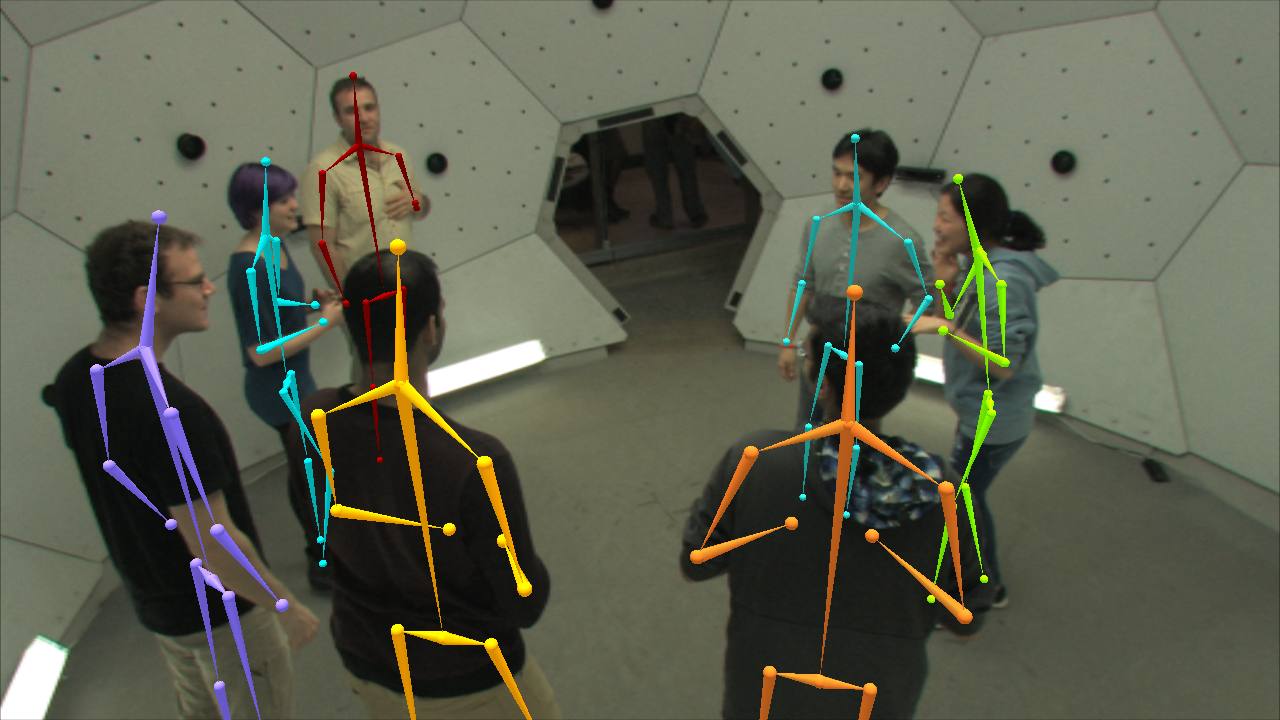
\includegraphics[width=\textwidth]{figures/0807_quant_noLegend/seven}
		\caption{Seven people}		
		\end{subfigure}
		

%	\subfloat{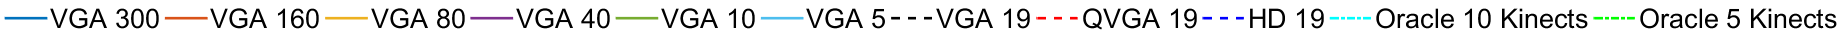
\includegraphics[width=0.9\textwidth]{figures/0822_quant_noLegend/legend}} 
%	\subfloat{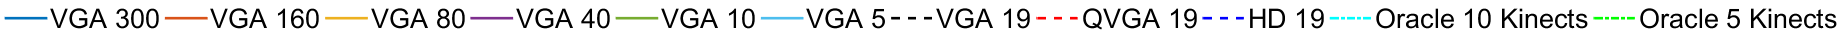
\includegraphics[width=0.9\textwidth]{figures/0822_quant_noLegend/legend}} 
	\caption{Performance evaluation using Probability of Correct Keypoint (PCK) metric for varying number and type of cameras on \emph{160422 ultimatum1}. We use the result of 480 VGA cameras after manually excluding outliers as ground truth. The X-axis of each graph represents thresholds, and the Y-axis represents accuracy by the thresholds. Each graph is generated for scenes with a different number of people. The results demonstrate that more views (rather than higher resolution) are beneficial to improve accuracy, and the distinction is more noticeable if the scene contains more people.} 
	\label{fig:quant1}
\end{figure}


%	\begin{table} [t]	
%		\centering
%		\caption{Summary of the Panoptic Studio dataset.}\label{Table:socialDataset}
%		
%		\begin{tabular}{c|c|c|c}
%			\hline 
%			Sequence Type & Subjects  & Sessions  & Duration  \tabularnewline
%			\hline 
%			Mafia & 4-8 & 7 & 78 min \tabularnewline
%			\hline 	
%			Ultimatum  & 2-8 & 36 & 47 min\tabularnewline
%			\hline 	
%			Haggling & 3 & 16 & 21 min \tabularnewline
%			\hline 	
%			007-Bang & 5-7 & 2 & 12 min \tabularnewline
%			\hline 	
%			Meeting & 6-8 & 1 & 10 min  \tabularnewline
%			\hline 	
%			Toddler &  2  & 1 & 5 min \tabularnewline		%150129_Ultimatum7
%			\hline 	
%			Dancer &  1  & 5 & 16 min   \tabularnewline		%150129_Ultimatum7
%			\hline 	
%			Cellist  & 1 & 1 &  5 min \tabularnewline		%150129_Ultimatum7
%			 \hline 	
%			Drummer & 1 & 2 & 4 min  \tabularnewline
%			\hline 
%			Total &   &  & 198 min 
%		\end{tabular} 
%	\end{table}
%	

\begin{table} [t]	
	\centering
	\caption{Processing time for one minute of data.}\label{Table:questionaire}
	\begin{tabular}{l | l|  r}
		\hline
		&  Procedure & Time  \tabularnewline
		\hline
		\multirow{4}{*}{Stage 1} & (\ref{subsection:nodeProposals}) 2D pose detection (1 GPU) &  40 h  \\
		
		&(\ref{subsection:nodeProposals}-\ref{subsection:partProposals})  Node and part proposal recon. (1 GPU) &  4 h  \\
		
		&(\ref{subsection:dynamicProgamming}) Skeletal proposal reconstruction by DP  &  3 m  \\
		
		&(\ref{subsection:dynamicProgamming}) Skeletal proposal optimization  &  11 m  \\
		\hline
		\multirow{2}{*}{Stage 2} & (\ref{subsection:patchTrajectoryRecon}) Trajectory stream recon. (400 CPU cores)  &  35 h  \\ % 31.5 + 3.5 (init)
		& (\ref{subsection:trajectoryAssociation}) Trajectory association and refinement &  5 m  \\
		%Depth Map generation  &  8 h  \tabularnewline
		%Patch Initialization  &  24 h  \tabularnewline
		\hline
	\end{tabular} 
	\label{table:processingTime}
\end{table}

\subsection{Processing Time}
The time to process one minute of data (1500 frames) of 480 VGA views is summarized in Table~\ref{table:processingTime}. We use different computing devices for procedures.  A machine with Intel i7 3.4GHz processor and 32GB RAM is used for general processing, a GTX Titan X is used for GPU computation, and a cluster server with 400 CPU cores (2.2GHz per processor) is used for trajectory stream reconstruction. 

In the first stage, most of the time is spent in running the 2D body pose detector. The detector runs at about 5 frames per second on a single GPU, but due to the large number of views (720K images per minute),  processing a minute of video takes about 40 hours. In practice, we use multiple GPUs to process multiple images in parallel. In the second stage, the main computational bottleneck is the trajectory stream generation. Although they are tracked in parallel, the running time is long due to the large number of patches at each time. In our experiments, on average 15K patches are tracked per person. 

\begin{table} [t]	
	\centering
	\caption{Quantitative evaluation of the accuracy of our method on the \emph{160422 ultimatum1} sequence. }\label{Table:otherDataset}
	\begin{tabular}{c|c|c|c|c}
		\hline 
		%		{Identity \#} & {Skeleton \#} & {Joint \#} & {Outlier \#} & {Missed \#} & {Accuracy}\tabularnewline
		{Skel. \#} & {Node \#} & {Outlier Node \#} & {Node Acc.}  & {Skel. Acc.} \tabularnewline
		\hline 
		81,829 & 1,227,435 & 8700 & 99.29\% & 93.55\% \tabularnewline
		%		 61 & 81,829 & 1,227,435 & 7,931 & 769 & 76555 & 99.29\% \tabularnewline
		\hline 
	\end{tabular} 
	\label{table:quant_stat}
\end{table}


\subsection{Performance Analysis 3D Body Motion Capture}
%Claim: Massively multiview overcomes problems of inter-occlusions
%+ Performance versus the number of views
%+ Performance versus camera resolution (we don't currently have this)
%\subsection{Quantitative Evaluation}
%+ Comparison with Kinect

We quantitatively evaluate the performance of our method for the \emph{160226 ultimatum1} sequence by varying the number and type of cameras. We choose the ultimatum sequence because it captures varying number of people (from two to seven people) in each time period, which is suitable to study the relation between scene complexity and the number of cameras needed to reach a desired performance. In this experiment, we only evaluate the first stage of our method.  

\textbf{Performance using all VGA cameras}: We first quantify the performance of our system when all 480 VGA cameras are used. Due to the absence of ground truth data, we manually annotate the correctness of the reconstructed 3D skeletons by verifying their projections in multiple 2D views. We labeled a 3D joint node as an outlier if the node is projected outside of the corresponding limb or far from the presumable target joint in multiple 2D views. We exclude the period where people come in and out of the system, since at the moment body parts lie on the edge of our system's working volume. The result of the quantitative evaluation for the 15 min of sequence is summarized in Table~\ref{table:quant_stat}. There are 12 sessions in the sequence, and 61 temporally associated skeletal structures are reconstructed. Among about 1.2 million body joints, about 8.7K nodes are determined as outliers or missed (rejected by thresholds of our system), showing 99.29\% accuracy in node reconstruction. And, 93.55\% out of about 82K 3D skeletons are correctly reconstructed without any incorrect joints. The majority of the failures are caused by insufficient visibility of the target part. An example is the pose holding hands behind one's back near the wall of the system as shown in Figure \ref{fig:failures} (left). Although the hands are visible from few cameras, they are too close to be detected by the pose detector. Interestingly, our method still reconstructs the hands using the ``guessed" 2D locations from 2D pose detector in frontal views, although the accuracy is limited as shown in Figure \ref{fig:failures}.

\textbf{Comparison with varying number of cameras}: To evaluate the impact of the number of views, we perform our method using varying number of cameras. The cameras are uniformly sampled (except the 19 VGA camera case explained later); i.e., we sample the next camera as the one furthest from all the already sampled cameras, and, thus, the selected cameras are always a subset of the set of the larger number of cameras. To quantify the results, we treat the result with 480 VGA cameras as ground truth after excluding the manually annotated outliers. For evaluation, we only use every tenth frame to reduce computation time. As an evaluation metric, we use the PCK (Probability of Correct Keypoint) metric, which is commonly used to evaluate 2D pose detectors~\cite{Andriluka-14}. Here, we use 3D distance in physical scale (cm) obtained from calibration data for the threshold of PCK, in contrast to the 2D ratio of torso/head as in 2D pose detection cases~\cite{Andriluka-14}. Figure~\ref{fig:quant1} shows the PCK accuracy by varying the camera number on the scenes with different number of people. In all the results, we find that using a larger number of views is beneficial. If the scene is simpler (e.g., the case with two or three people), we observe that the results with a smaller number of cameras, e.g., 160 cameras, show a similar performance with 480 cameras. However, if the scene becomes more complicated, e.g., seven people, we see clearer gaps according to the camera numbers. This results can be meaningfully used to design a multiple camera system to determine the required number of cameras given a desired group size. For example, assuming that the target scenes have about five people, we forecast that a system with 80 cameras can reach about 94\% of accuracy with a 2cm threshold. 


\begin{figure}[t]
	\centering
	\captionsetup{position=top}
	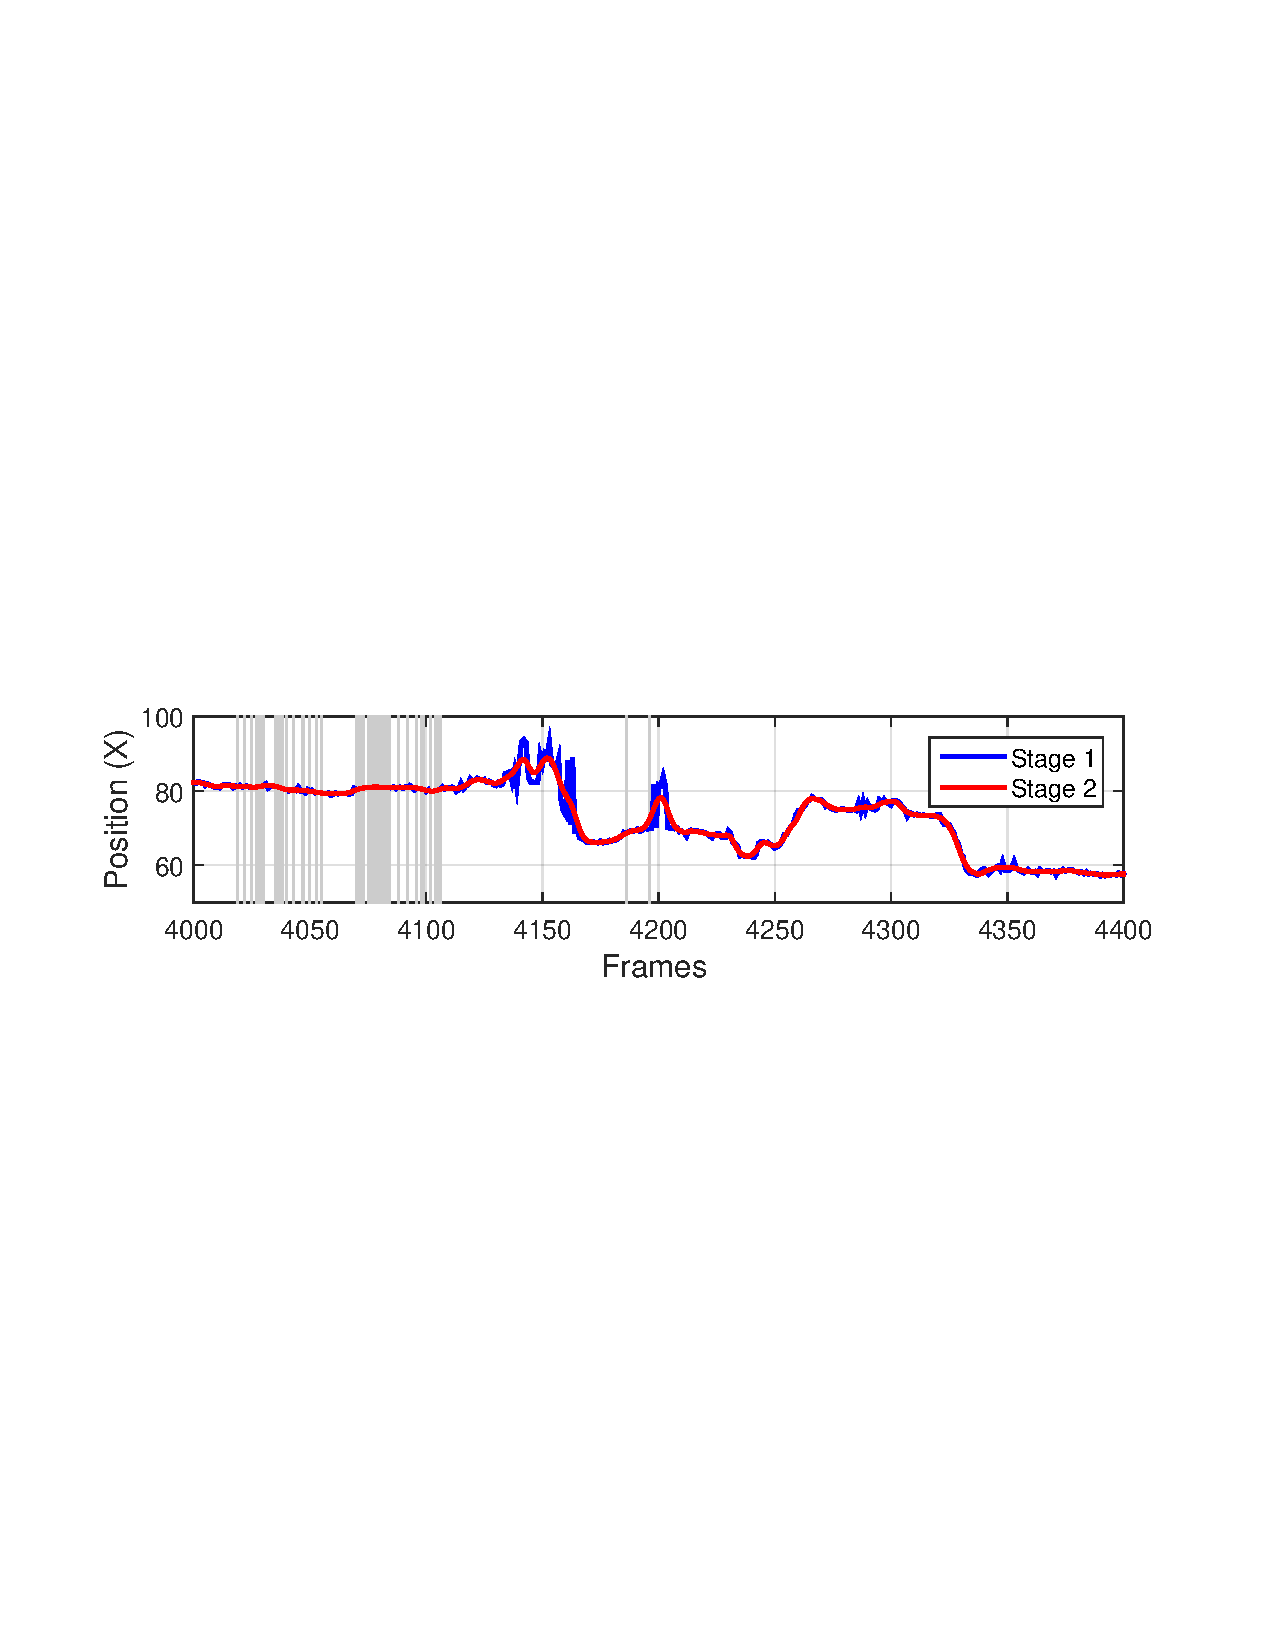
\includegraphics[trim=40 340 60 340,clip,width=\linewidth]{figures/quant_stage2/160226_mafia2-Stage2-nodeLocation-h7-j11-1.pdf}   \\
	%\subfigure[Y Coordinate]{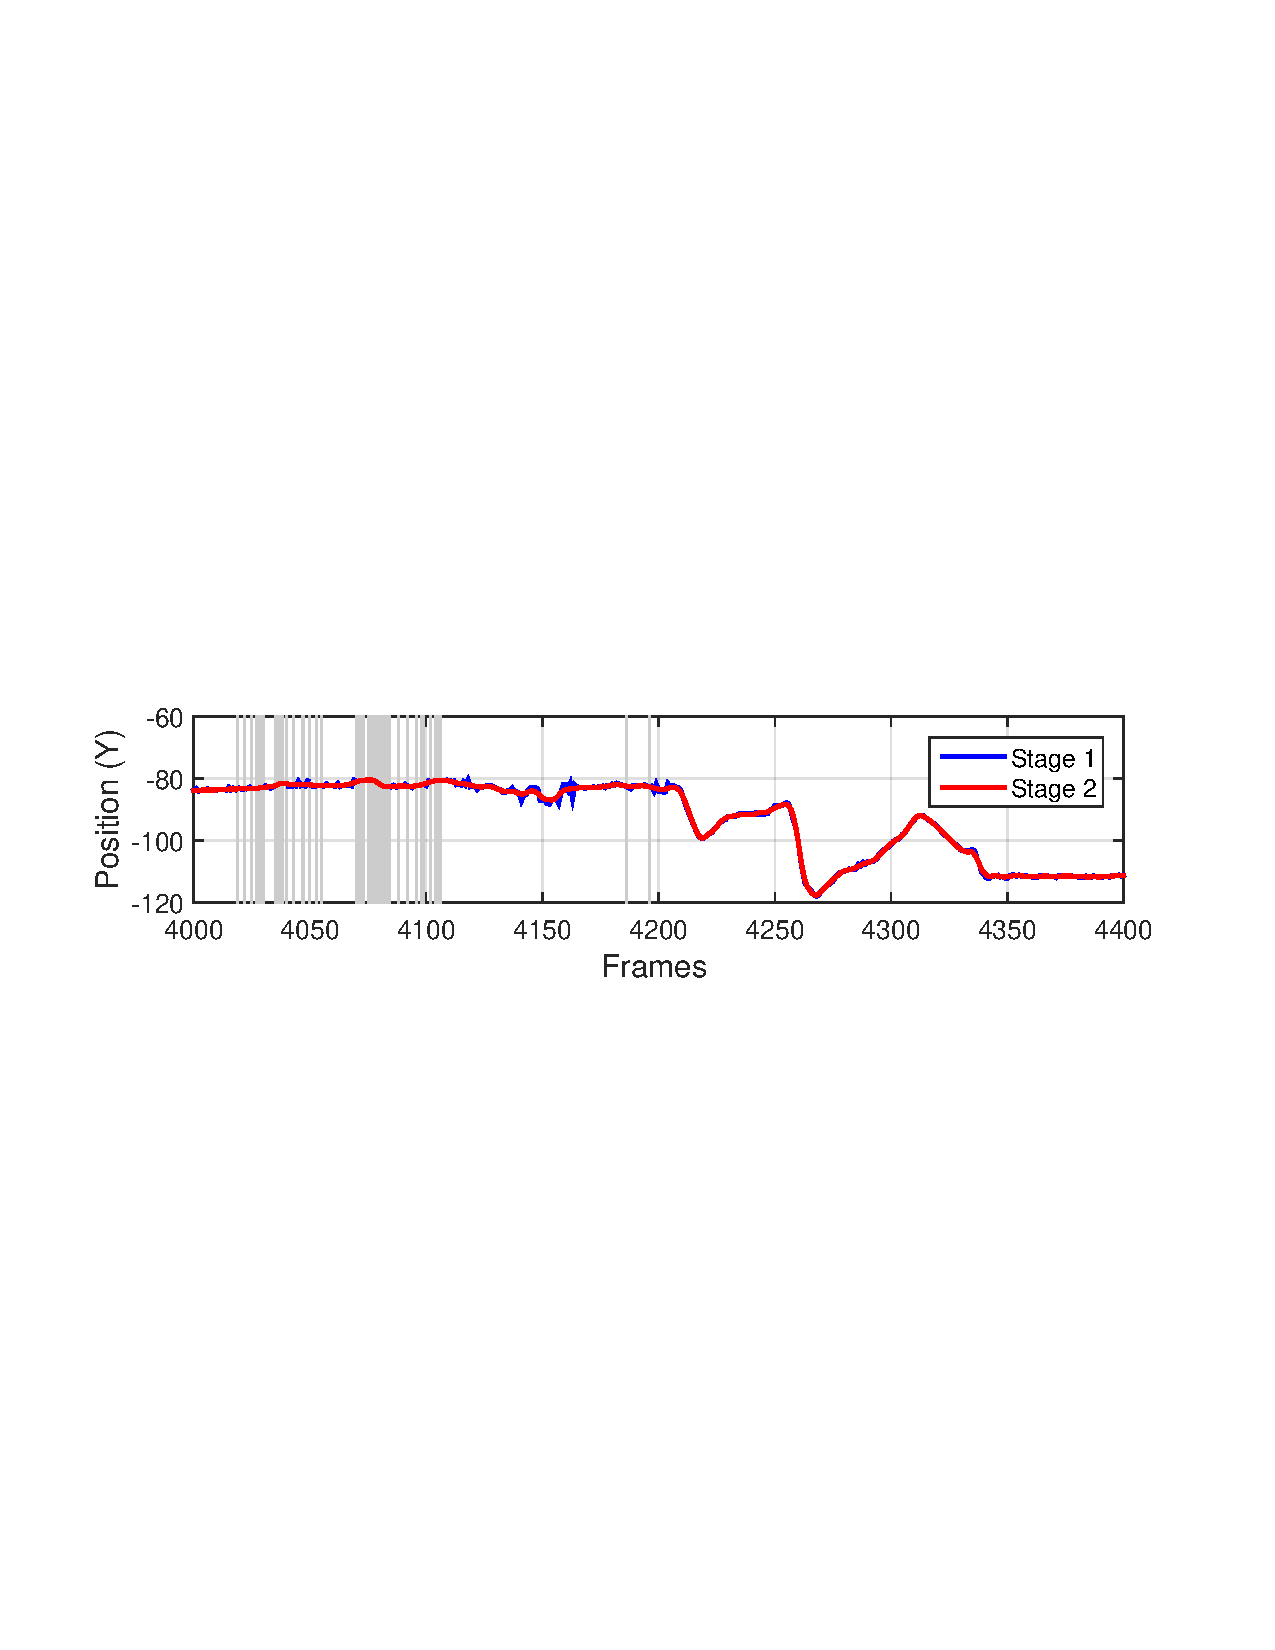
\includegraphics[trim=40 340 60 340,clip,width=\columnwidth]{imgs/quant/stage2/160226_mafia2-Stage2-nodeLocation-h7-j11-2.pdf}}   \\
	%\subfigure[Z Coordinate]{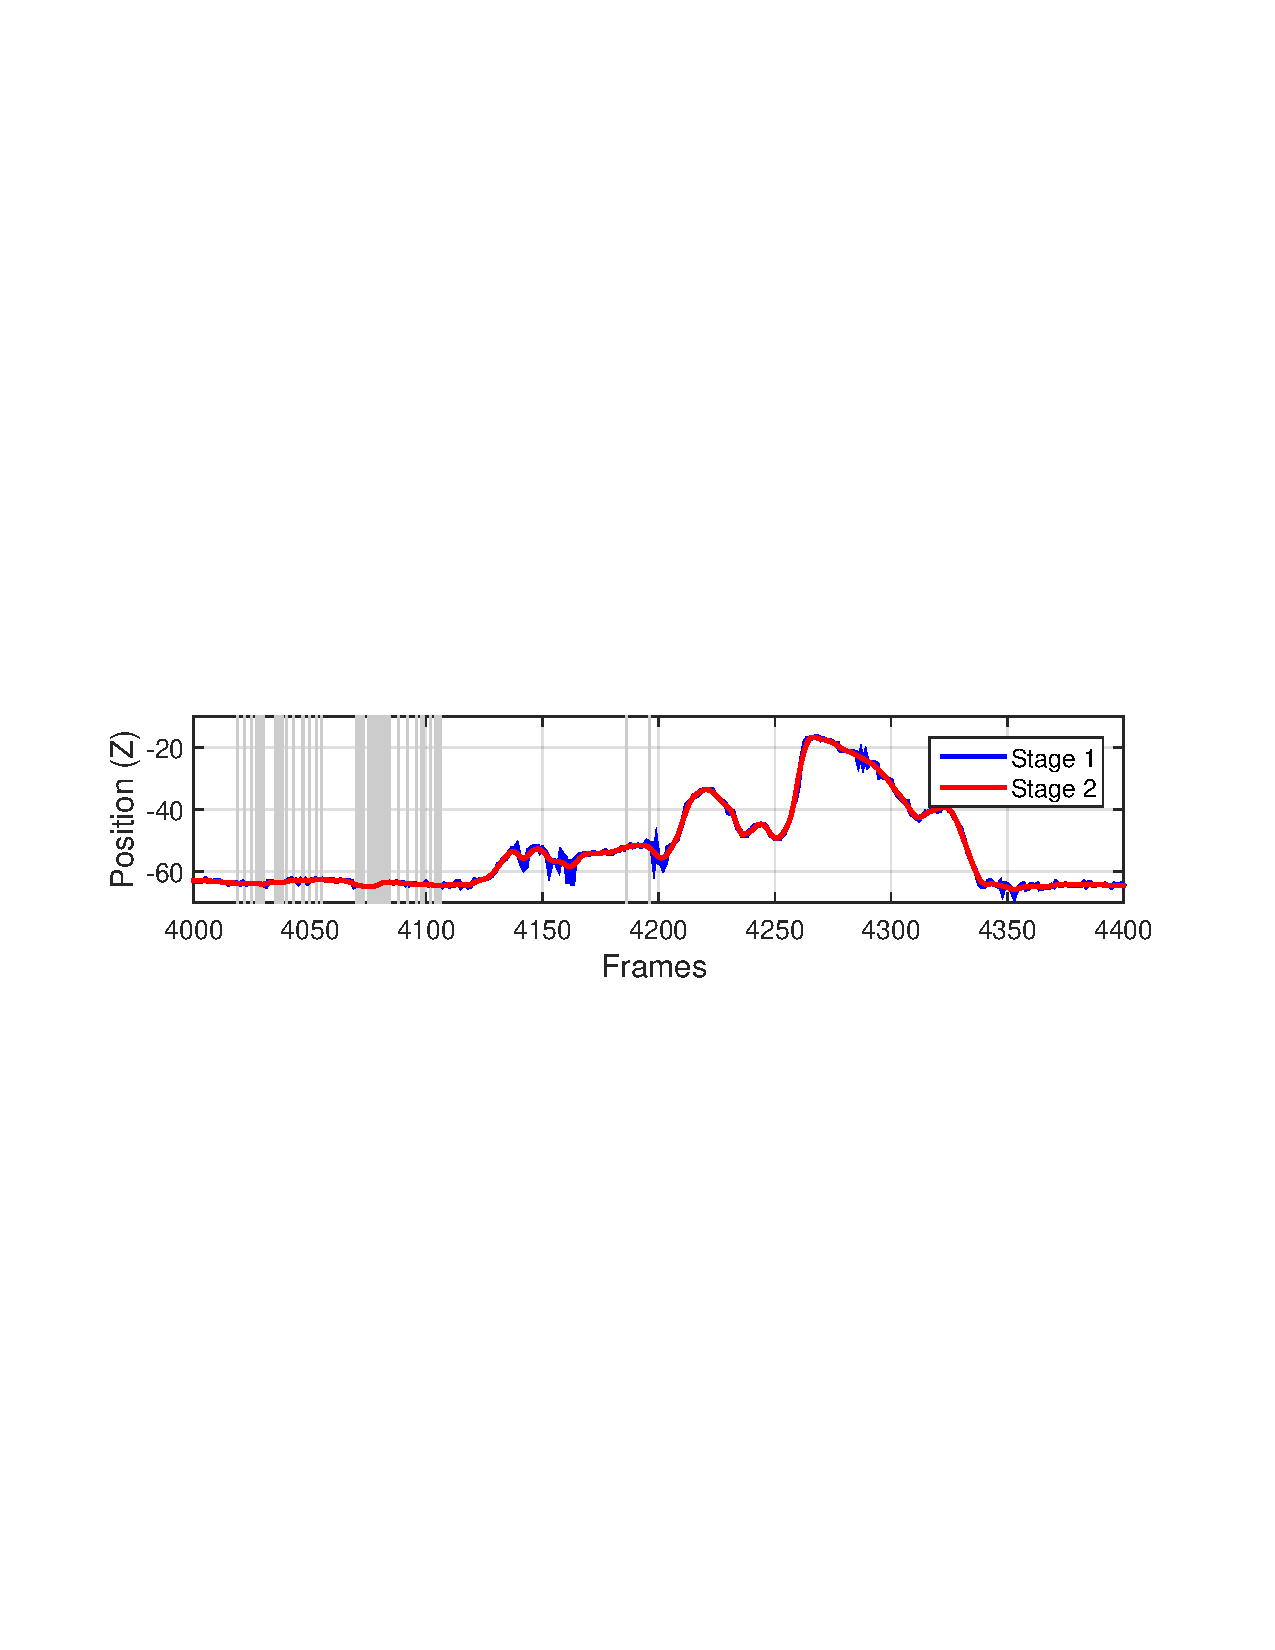
\includegraphics[trim=40 340 60 340,clip,width=\columnwidth]{imgs/quant/stage2/160226_mafia2-Stage2-nodeLocation-h7-j11-3.pdf}}   
	%	\subfigure[Seven people]{\label{Fig:quant2-1}\includegraphics[trim=40 180 60 170,clip,width=0.24\textwidth]{imgs/quant/0720_quant_noLegend/PCK-Threshold-seven-people.pdf}} 
	%	\subfigure{\includegraphics[width=0.8\textwidth]{imgs/quant/0720_quant_noLegend/GraphColorLegend}} 
	\caption{Refinement result by the Stage 2 of our method on the \emph{160226 mafia2} sequence. The most erroneous node is selected. The graph represents the X coordinate of the node across frames after the Stage 1 method (blue) and Stage 2 method (red). The gray regions represent the frames where the part is missing in the stage 1 output. They are recovered via the temporal propagation in the result of Stage 2. } 
	\label{fig:quant_stage2}
\end{figure}


%Figure~\ref{fig:quant1} shows the same result in a different graph format. In each graph, we fix the threshold to determine pck, and plot PCK performance versus number of cameras for each scene with different number of people. It is clearly scene that having more cameras are beneficial if we want to get higher accuracy as 1cm error from the GT data, especially a scene is more complicate. If we consider loose error such as 5cm, we see saturation from lower number of cameras. These results are particularly useful when a system is designed with a goal. For example, if we need a multiple view system to get a 0.95 PCK@2cm error for four number of people case, we can forecast that around 80 cameras is needed assuming the working volume space with 5 m radius.

\textbf{Comparison with varying resolutions}: As an additional evaluation, we perform a similar experiment for different camera resolutions using the multiple HD cameras installed in our system. Among 31 HD cameras, we use 19 HD cameras installed on the same panels with VGA cameras\footnote{We have 20 HD cameras installed on the same panels with VGAs, but we missed 1 HD camera due to the hardware failure during the capture.}.  To compose similar viewpoints, we choose the closest VGA cameras from the selected 19 HDs. Additionally, we generate 19 QVGA inputs (320 $\times$ 240 resolution)  by resizing the selected VGA videos. Because the HD cameras are not perfectly synchronized with VGAs, we interpolate the result from HDs into VGA time domain using the hardware sync data. The performance of a same number of HDs, VGAs, and QVGAs is shown as dashed lines in Figure~\ref{fig:quant1}. The result shows that the performance differences among them is marginal, although HD views have about 7 time more pixels than VGAs and about 27 times more pixels than QVGAs. The result demonstrates that the pose reconstruction performance of our method is marginally affected by the resolution changes compared to the changes by the number of views. Note that the integral of number of pixels in the 19 HD views are equivalent to about 128 VGA views, and the result clearly shows that it is more advantageous to have more unique camera views rather than having higher resolutions, given a fixed pixel budget. The main reason underlying this finding is that dealing with occlusions is more crucial in interaction capture scenarios, and, in particular, higher resolution is not beneficial in our method, since 2D joint localization accuracy is still limited by the 2D pose detector.

\textbf{Comparison to multiple Kinects}: We also compare our results with the result of multiple Kinects. Since Kinect with its accompanying SDK is one of the most commonly used sensors for markerless motion capture in various communities, using multiple Kinects can be considered as an option to handle severe occlusions for interaction capture. However, how to fuse multiple Kinect cues is not straightforward, and, thus, we naively fuse them as follows. We first generate 3D skeletal proposals from all individual Kinects, and simply find the best candidate closest to our ground truth data in Euclidean space, assuming that an Oracle chooses the best one given the GT data. This can be considered an upper bound of a naive multiple Kinects method. Since the keypoint locations of the Kinects are not identical to the skeletons of our method, for a fair comparison, we adjust the Kinect skeletons by finding an offset vector from each Kinect node toward our node of GT's skeleton in a person-centric coordinate system. As shown in Figure~\ref{fig:quant1}, the results of the \emph{Oracle} Kinects is limited, showing less than 80\% accuracy at a 5cm threshold. % More specifically, an offset at a time instance is simply computed by differencing the GT's node and Oracle Kinect's node, and they are transformed to a person centric coordinate. To the end, the final offset is computed by averaging the offset vectors obtained across time. Since the person centric coordinate is defined by a torso point, we apply this adjustment only for the torso and head nodes. 

\subsection{Refinement by Trajectory Stream}
%Claim: Massi

%\textbf{Refinement by the second stage}: 
We compare the performance improvement of our refinement method (the second stage) over the output of the first stage. We choose a  challenging scene in \emph{160226 mafia2} sequence where the first stage of our method shows failures due to the erroneous 2D pose detection results. To see the performance change, we plot the X coordinate of the most erroneous node (right wrist of a subject) as shown in Figure~\ref{fig:quant_stage2}. The frames denoted as gray regions are the time when the nodes are missed due to the consistent 2D pose detector failures. It is shown that our refinement method can recover the missing parts and also noticeably reduce the motion jitter for the unstable frames. Note that our refinement method is not just smoothing but based on the temporal transformation measured by a dense trajectory stream. Thus, it does not suffer from over-smoothing, even after several iterations. %See the time around the frame 4250 in Figure~\ref{fig:quant_stage2} where the curves are retained as original after 5 iterations in this example. 
%
%
%\begin{table} [t]	
%	\centering
%	\caption{Questionnaire.}\label{Table:questionaire}
%	\begin{tabular}{c|c|c|c|c|c|c}
%		\hline 
%		{Strongly not bias} & {Not biased} & {Borderline} & {Biased} & {Strongly biased} \tabularnewline
%		\hline 
%		16\% (2) & 50\%(6) & 25\% (3) & 8.3\% (1) & 0 \% \tabularnewline
%		\hline 
%	\end{tabular} 
%	\label{table:questionaire}
%\end{table}
%
%
%\subsection{Comparison with The Method of Joo et al.~\cite{Joo-15}}
%We compare the presented method to the method introduced in \cite{Joo-15}. In \cite{Joo-15}, due to the relatively unreliable 2D pose detection cue~\cite{Yang-2012}, the motion cues from trajectory stream play a core role to reconstruct valid parts. The method, however, tends to fail in regions where the trajectory stream is unavailable (e.g., the texture-less dark body parts). The method presented in this paper is composed of two sequential stages using an advanced 2D pose detector~\cite{Wei-2016}, and Stage 1 is still applicable in the region where trajectory stream is unavailable. Table~\ref{Table:iccvComparison} shows the comparison between two methods on the sequence \emph{150129 007-Bang} introduced in \cite{Joo-15}, where the accuracy is computed by manually annotating outliers. The major failures of \cite{Joo-15} occur on the texture-less leg parts, or fast motion with motion blur when the trajectory stream is sparse and inaccurate. Refer to the supplementary video for the qualitative comparison. %The first stage of our method still can be applied for those regions, although further refinement of the second stage is limited.

\begin{table} [t]	
	\centering
	\caption{Quantitative comparison to \cite{Joo-15} on the \emph{150129 007Bang} sequence. }
	
	\begin{tabular}{c|c|c|c|c|c}
		\hline 
		{Methods} & {Frames} & {Joints} & {Outliers} & {Missed} & {Accuracy}\tabularnewline
		\hline 
		Ours & 300 & 22,500 & 1 & 0 & 99.99\% \tabularnewline
		\hline 
		%		 \cite{Joo-15} & 300 & 22,500 & 1850 & 14 & 91.72\% \tabularnewline
		\cite{Joo-15} & 300 & 22,500 & 1871 & 2248 & 80.80\% \tabularnewline
		\hline 
	\end{tabular} 
	\label{Table:iccvComparison}
\end{table}

%\begin{figure}[t]
%	\centering       
%	\subfigure[Method of \cite{Joo-15} ]{\includegraphics[width=0.45\columnwidth]{imgs/iccvCompare/iccv_traj_frm_04720}} 
%	\subfigure[Our Method]{\includegraphics[width=0.45\columnwidth]{imgs/iccvCompare/pami_traj_frm_04720}} 
%	\caption{Qualitative comparison to \cite{Joo-15} on the \emph{150129 007Bang} sequence. Note that legs are missing in the result of \cite{Joo-15} due to the lack of trajectories. In the result of \cite{Joo-15}, left-right limbs are not consistently determined because the pose detector used does not provide this information. We ignore the confusion when we count outliers. } 
%	\label{fig:iccvComparison_fig}
%\end{figure}

%  \begin{figure*}[t]
%  	\includegraphics[width=\linewidth]{imgs/qualitative_trajLabel}
%  	%\includegraphics[width=\linewidth]{images/Design6.pdf}
%  	\caption{Trajectory labeling by the stage 2 of our method on \emph{160226 ultimatum1} (top) and \emph{160226 mafia2} (bottom). Each column shows the scene at a time instance. Each color represent each body part as in Figure~\ref{fig:overview}. }\label{fig:traj_labeled}
%  \end{figure*}


% \begin{figure*}[t]
% \includegraphics[width=\linewidth]{imgs/0807_qualitative}
% %\includegraphics[width=\linewidth]{images/Design6.pdf}
% \caption{ Motions of multiple people are captured by using the stage 1 of our method with 480 VGA cameras. For each result, the left image shows the reprojected skeletons on a novel HD view which is not used for the reconstruction. The image on the right shows a 3D rendering in another novel view. (row 1-3) \emph{160226 ultimatum1}; (row 3-5) \emph{160422 ultimatum1}; (row 6) \emph{151125 mafia1}.}
% \label{fig:qualitativeSocial}
% \end{figure*}

%  \begin{}[t]
%  	\includegraphics[width=\linewidth]{imgs/qualitative_trajLabel}
%  	%\includegraphics[width=\linewidth]{images/Design6.pdf}
%  	\caption{Trajectory labeling by the stage 2 of our method on \emph{160226 ultimatum1} (top) and \emph{160226 mafia2} (bottom). Each column shows the scene at a time instance. Each color represent each body part as in Figure~\ref{fig:overview}. }\label{fig:traj_labeled}
%  \end{figure*}

\subsection{Qualitative Evaluation For Body Motion Capture}
We apply our method, producing about 3 hours of interaction capture results. Due to the computation time, the second stage of our method is applied on a subset of the dataset; yet the first stage of our method is applied on all the sequences\footnote{Results will be updated in our website, as they are processed.}. Example results are shown in Figure~\ref{fig:qualitativeSocial}. Our result is fully automatic---given video streams and calibration data, our method generates temporally associated 3D skeletons (and labeled patch trajectory stream of each body part if the second stage is applied) for each individual without any human supervision. Refer to the supplementary videos and the live 3D viewer on our website. 

\textbf{Group interaction capture}: Our method produces motion capture results on various social game scenarios performed by multiple people (up to 8 people). The number of subjects in the scenes is automatically determined by our method, and allowed to vary during the capture. The reconstructed results contain motions that frequently occur during communication, such as crossed-arms-on-chest, resting-chin-on-hand, mouth-guard, hands-on-back, hands-on-waist, and so on. In spite of their importance as non-verbal signals transmitting a variety of messages, such motions get little attention by prior work. In particular, severe topological changes and self-occlusions make it hard to apply 3D template-based motion capture approaches. Our method reconstructs the motion of such challenging scenes by fusing 2D pose detection cues and motion cues using a larger number of views, and demonstrates a compelling performance for social interaction capture. %There are many other subtle gestures unconsciously performed by people, including rolling-up-sleeves and scratching-arms. For some sequences, a person is tying shoelaces and people suddenly do rock-paper-scissors to make decision. It is demonstrated that our method robustly reconstructs all of the above interesting non-verbal cues. %Another interesting characteristic of our results is the voluntarily induced geometrical formations of people, which is known as F-formation~\cite{Kendon-90}. Since our dataset capture the time where people enter the system, it is also reconstructed that how people make the formations according to different games and different roles. 

\textbf{Robustness to appearance, body sizes, and topological changes}: 
Our results demonstrate robustness to subjects of diverse appearance, body types, and sizes. As mentioned, subjects' clothing is not controlled, and the captured sequences contain people with various clothing such as black pants, thick padding jumpers, hoodies, short pants, scarfs, and so on. During the discussions, they also unconsciously adjust their clothing, for example by rolling up sleeves or relocating scarfs. The height of subjects varies from a two-year old toddler to adults more than 190 cm tall. The ``model-free" nature of our method enables us to reconstruct their motions without changing any parameter. It demonstrates a major advantage of our system for social behavior studies in that it can be easily applied for captures at scale, without any laborious template generation or initial alignment step. Especially, the toddler scene is challenging to  ``model-heavy" approaches, since instructing young children to be stationary to generate their template models (e.g., laser scanning) may not be practical. 

%\textbf{Various scales}: Since our method does not make assumption about the subject's height, the same method can be applied for tall adults and toddlers.  For example our dataset captures tall people as shown in~\ref{fig:qualitativeSocial}, and a toddlers as shown in Figure~\ref{fig:qualitative_nonsocial} top. However, we see that the result of the toddler is relatively unstable because: (1) the toddler is small and only limited views can see him; (2) the 2D pose detector of \cite{Wei-2016} is trained mainly by adult's body poses~\cite{Andriluka-14}. 

\textbf{Other interesting scenes}:
We also demonstrate the performance of our method on other atypical motion capture scenarios including musical performances (\emph{drummer} and \emph{cellist}) and \emph{dancer} sequences. Motion capture for musical performance is a good application for markerless motion capture, because markers may interfere with their functional movements during the capture. Although the scenes are challenging due to the severe occlusions by musical instruments, our method shows good performance in reconstructing the performer's subtle motions (e.g., the vibrato motion in the \emph{cellist} sequences).

On the other hand, the \emph{dancer} sequences contain fast motion and unusual poses. Due to failures in reconstructing the trajectory stream for the extremely fast movement compared to our relatively low frame rate cameras (25 Hz), we only apply the first stage of our method. Separating reconstruction (Stage 1) from temporal refinement (Stage 2) is advantageous in this case, because the first stage, based on per-frame reconstruction, is not affected by motion magnitude and free from error accumulation. We can optionally apply temporal refinement (Stage 2) based on the quality of trajectory stream to further refine the results. We find that, however, in a few extremely unusual poses our method becomes unstable due to consistent 2D pose detection failures, which will be discussed in subsection~\ref{subsection:Limitation}. 


% \textbf{Semantic labeling of dense patch trajectories}: As output of the stage 2 of our method, the semantically labeled dense trajectories are obtained as shown in Figure~\ref{fig:quant_stage2}. The labeled trajectories captures the subtle deformation of the body limbs across time. 


%\begin{figure*}[t]
%	\centering
%	\subfigure[160226-mafia1]{\includegraphics[width=0.24\textwidth]{imgs/qualitative/160226_mafia1/00008528_00_06}}   
%	\subfigure[160226-mafia1]{\includegraphics[width=0.24\textwidth]{imgs/qualitative/160226_mafia1/00003}}  
%	\subfigure[160226-mafia1]{\includegraphics[width=0.24\textwidth]{imgs/qualitative/160226_ultimatum1/00011716_00_11}}   
%	\subfigure[160226-mafia1]{\includegraphics[width=0.24\textwidth]{imgs/qualitative/160226_ultimatum1/00001}}   
%	\subfigure[160226-mafia1]{\includegraphics[width=0.24\textwidth]{imgs/qualitative/160226_haggling1/00000810_00_20}}   
%	\subfigure[160226-mafia1]{\includegraphics[width=0.24\textwidth]{imgs/qualitative/160226_haggling1/00000}}   
%	\subfigure[160226-mafia1]{\includegraphics[width=0.24\textwidth]{imgs/qualitative/160317_meeting1/00005081_00_01}}   
%	\subfigure[160226-mafia1]{\includegraphics[width=0.24\textwidth]{imgs/qualitative/160317_meeting1/00001}}   	
%	\subfigure[160226-mafia1]{\includegraphics[width=0.24\textwidth]{imgs/qualitative/ian2/00003202_00_02}}   
%	\subfigure[160226-mafia1]{\includegraphics[width=0.24\textwidth]{imgs/qualitative/ian2/00001}}   		
%	\subfigure[160226-mafia1]{\includegraphics[width=0.24\textwidth]{imgs/qualitative/cello4/00004937_00_11}}   
%	\subfigure[160226-mafia1]{\includegraphics[width=0.24\textwidth]{imgs/qualitative/cello4/00001}}   	
%	\caption{Qualitative Results} 
%	\label{fig:qualitative}
%\end{figure*}



%  \begin{figure*}[t]
%  	\subfigure{\includegraphics[width=\textwidth]{imgs/160401_ian3_sequence}}   
%  	\subfigure{\includegraphics[width=\textwidth]{imgs/150821_dance3_sequence}}   
%  	%\includegraphics[width=\linewidth]{images/Design6.pdf}
%  	\caption{Motion capture results of \emph{160401 ian3} and \emph{150821 dance1}. Our method can be applied to reconstruct the subjects of arbitrary height, from toddlers to adults as demonstrated in the \emph{160401 ian3}. The challenging fast and unusual poses in the \emph{150821 dance1} sequence are also reconstructed. }\label{fig:qualitative_nonsocial}
%  \end{figure*}
%
%\begin{figure*}[t]
%	\includegraphics[width=\linewidth]{imgs/qualitativeOthers}
%	%\includegraphics[width=\linewidth]{images/Design6.pdf}
%	\caption{Motion capture results of \emph{150303 cello3} and \emph{150406 drum4}. Using our massively multview system, our method can reconstruction the motions of musical performers in spite of the severe occlusions by the musical instruments.}\label{fig:musical}
%\end{figure*}
%

%\begin{itemize}
%    \item Pose detection: 9.5 hours using 4 GPUs (GTX TitanX)  --> 38 hours
%    \item Pose detection merging: 1.5 hours
%    \item Node and part proposal generation: 4 hours using 1 GPUs
%    \item DP:  3 min
%    \item Optimization: 11 min
%    \item Trajectory Stream: +-30frames, 10frames --> 93 hours
%	\item Depth Rendering: 10 kinect views 8 hours 
%	\item Patch Initialization: 24 hours
%	\item Stage 2: 5 min /iteration
%\end{itemize}


\begin{figure}[t]
	\centering
	\includegraphics[width=\linewidth]{figures/FailureCases3}
	%\subfigure[]{\includegraphics[trim=0 0 1000 0,clip,height=0.23\columnwidth]{imgs/160422UltimatumFailures}}   
	%\subfigure[]{\includegraphics[trim=800 0 0 0,clip,height=0.23\columnwidth]{imgs/160422UltimatumFailures}}   
	\caption{Example failure cases. For each column, the first row shows the projection of reconstructed 3D skeletons on a view where the red colored parts are manually annotated outliers. The second row shows the 2D pose detection results. (Left) The hands are severely occluded and only visible from few cameras where they are too close to be detected by 2D pose detector. (Center) The left/right legs are confused in performing 2D pose detection, which causes failures in our 3D inference. (Right) The toddler is not detected by the pose detector, since he is severely occluded. }\label{fig:failures}
\end{figure}


\begin{figure}[t]
	\centering
	\includegraphics[trim=0 0 0 0,clip,width=\linewidth]{figures/0916_qualitative}
	%\includegraphics[trim=0 0 0 140,clip,width=\linewidth]{imgs/0807_qualitative}
	%\includegraphics[width=\linewidth]{images/Design6.pdf}
	\caption{ Our method is performed on various scenes including social interactions of multiple people. (Row 1) Reprojected skeletons on novel HD views; (Row 2) Rendered 3D skeletons in novel 3D views with node trails over time; (Row 3) Labeled 3D trajectories representing articulated non-rigid body parts with same color representations as in Figure \ref{fig:overview}; (Row 4-7) Reprojected skeletons on novel HD views of various scenes.}
	\label{fig:qualitativeSocial}
\end{figure}

\subsection{Qualitative Evaluation For Hand and Face Motion Capture}
The reconstruction results of 3D hands and faces are shown in the Figure~\ref{fig:qualitativeHandCaptureGroup} and \ref{fig:qualitativeFullMocap}. We only use 31 HD views for the reconstruction due to the limited image resolution of VGA views. Compared to prior work on high-quality face reconstruction where entire cameras mainly focus on a face~\cite{beeler2010high},  the cameras in our system have much wider field of views to capture full body motion of multiple people, and, thus, the quality of our face reconstruction is limited and produces only a fixed number of landmark locations (70 points determined by 2D face detector). Yet, our system shows a reasonable performance in capturing facial expressions of interacting people.

Our 3D hand capture is the first in capturing hand gestures of interacting multiple people in a practical level, which is even challenging in state-of-the-art marker based motion capture system. Especially, we also found that our hand capture shows a great performance in capturing hand motion interacting with objects as shown in Figure~\ref{fig:qualitativeHandCaptureGroup}, despite limited camera resolutions.  Reconstruction results in capturing full body motion of hands, body, and faces of interacting multiple people are shown in Figure~\ref{fig:qualitativeFullMocap}, which is also demonstrated for the first time. 

\begin{figure}[h]
	\centering
	\includegraphics[trim=0 335 0 0,clip,width=0.85\textwidth]{figures/qual3d_singles}
%	\caption{Qualitative multiview results on sequences not used during bootstrapping. (a)~Reprojected triangulation. (b)~3D hands in context. (c)~Metric reconstruction. (d)~2D~detections from hand pose detector presented in~\cite{Tomas-17}.}
%	\label{fig:qualitativeHandCapture}
	\includegraphics[trim=0 150 0 0,clip,width=0.85\textwidth]{figures/qual3d_group_comp}
	\caption{Qualitative results on hand and body motion capture. (First 4 rows) (a)~Reprojected triangulation. (b)~3D hands in context. (c)~Metric reconstruction. (d)~2D~detections from hand pose detector presented in~\cite{simon2017hand}. (Last 4 rows) Hand and body motion capture of interacting multiple people.}
	\label{fig:qualitativeHandCaptureGroup}
\end{figure}
\vfill

\begin{figure}[h]
	\centering
	\includegraphics[trim=0 0 140 70,clip,width=0.49\textwidth]{figures/fullmocap/00000}
	\includegraphics[trim=0 0 140 70,clip,width=0.49\textwidth]{figures/fullmocap/00002}
	\includegraphics[trim=70 0 70 70,clip,width=0.49\textwidth]{figures/fullmocap/00008}
	\includegraphics[trim=70 0 70 70,clip,width=0.49\textwidth]{figures/fullmocap/00009}
	\includegraphics[trim=70 0 70 70,clip,width=0.49\textwidth]{figures/fullmocap/frm_04541}
	\includegraphics[trim=70 0 70 70,clip,width=0.49\textwidth]{figures/fullmocap/frm_04541-2}
	\includegraphics[trim=70 0 70 70,clip,width=0.49\textwidth]{figures/fullmocap/frm_10029}
	\includegraphics[trim=70 0 70 70,clip,width=0.49\textwidth]{figures/fullmocap/frm_10029-2}	
	\caption{Capturing anatomical landmarks from full body parts (face, body, and hand). (Left) An example scenes overlaid by the projection of reconstructed results (Right) Reconstruction results in 3D views. }
	\label{fig:qualitativeFullMocap}
\end{figure}
\vfill

\subsection{Limitations}
\label{subsection:Limitation}
A limitation of our method is the dependency on a 2D pose detection method. State-of-the-art pose detectors are weak in detecting unusual poses and closely located people (as shown in  Fig.~\ref{fig:failures}). We also find that the pose detector sometimes gets confused in distinguishing left-right limbs (as shown in the center of Figure~\ref{fig:failures}). Although our method can overcome these issues by fusing cues across views via spatial voting and across time via associating trajectory streams, if the 2D body pose detectors fail consistently, our method is unable to recover. The second limitation is the long computation time to process the large number of views. However, depending on the application, the computation time can be greatly reduced by using a smaller number of cameras with a trade-off in accuracy (see Fig.~\ref{fig:quant1}). 
%
%\section{Summary}
%In this chapter, we present the Panoptic Studio and an interaction capture method that leverages a large number of views. To demonstrate the performance of our method, we collect a large scale social interaction dataset, and produce compelling motion capture results on it. In particular, we empirically find that having a larger number of views is more beneficial than having a higher resolution of views for social interaction capture. Our quantitative comparison on various number and type of cameras can be used as a meaningful resource to design follow-up multiview systems to estimate the required number of views to achieve a desired accuracy. Our method also demonstrates that highly-occluded social motion capture is possible by boosting 2D pose detection cues and motion cues in a larger number of views, without using any heavy prior or template model. Our method shows its advantages in the social interaction capture scenario by reconstructing subjects of diverse appearance, body sizes, and body topology for a long term without error accumulation issue.
%

\clearpage




%\subsection{Future Work}
%There are various future directions expanding our system and outputs. First, analyzing human social behaviors using the measured social signals of our system is an interesting direction, which will facilitate social behavior understanding in a data-driven manner. Second, our interaction capture outputs can be used as labeled data to train new 2D detectors. By projecting the skeletal reconstruction outputs on all 521 views, our current dataset generates 153 million pose data in diverse views. Although the appearance diversity of the scenes would be limited compared to internet photos, our dataset is still meaningful in that: (1) it captures multiple interacting people showing severe inter-occlusions in the scenes; (2) it has annotations for entire video frames which is the key to study temporal relation of poses; (3) the scenes are taken by 521 diverse view points compared to the biased views of usual portrait photos (e.g., frontal views or side views). This type of labeled data would be hard to obtain by manual annotations. Lastly, a similar massively multiview approach can be applied to reconstruct 3D faces. This can be done by substituting the 2D body pose detector with a 2D face landmark detector in our method.
%

\pagebreak